% ******************************* PhD Thesis Template **************************
% Please have a look at the README.md file for info on how to use the template

\documentclass[oneside,a4paper,12pt,bookman,numbered,print,index]{Classes/CSEThesisPSnPDF}
\usepackage{booktabs}
%\usepackage[utf8]{inputenc} % This for vietnamese 
%\usepackage[utf8]{vietnam} % This for vietnamese 

% ******************************************************************************
% ******************************* Class Options ********************************
% *********************** See README for more details **************************
% ******************************************************************************

% `a4paper'(The University of Cambridge PhD thesis guidelines recommends a page
% size a4 - default option) or `a5paper': A5 Paper size is also allowed as per
% the Cambridge University Engineering Deparment guidelines for PhD thesis
%
% `11pt' or `12pt'(default): Font Size 10pt is NOT recommended by the University
% guidelines1z1
%
% `oneside' or `twoside'(default): Printing double side (twoside) or single
% side.
%	
% `print': Use `print' for print version with appropriate margins and page
% layout. Leaving the options field blank will activate Online version.
%
% `index': For index at the end of the thesis
%
% `draftclassic': For draft mode without loading any images (same as draft in book)
%
% `draft': Special draft mode with line numbers, images, and water mark with
% timestamp and custom text. Position of the text can also be modified.
%
% `abstract': To generate only the title page and abstract page with
% dissertation title and name, to submit to the Student Registry
%
% `chapter`: This option enables only the specified chapter and it's references
%  Useful for review and corrections.
%
% ************************* Custom Page Margins ********************************
%
% `custommargin`: Use `custommargin' in options to activate custom page margins,
% which can be defined in the preamble.tex. Custom margin will override
% print/online margin setup.
%
% *********************** Choosing the Fonts in Class Options ******************
%
% `times' : Times font with math support. (The Cambridge University guidelines
% recommend using times)
%
% `fourier': Utopia Font with Fourier Math font (Font has to be installed)
%            It's a free font.
%
% `customfont': Use `customfont' option in the document class and load the
% package in the preamble.tex
%
% default or leave empty: `Latin Modern' font will be loaded.
%
% ********************** Choosing the Bibliography style ***********************
%
% `authoryear': For author-year citation eg., Krishna (2013)
%
% `numbered': (Default Option) For numbered and sorted citation e.g., [1,5,2]
%
% `custombib': Define your own bibliography style in the `preamble.tex' file.
%              `\RequirePackage[square, sort, numbers, authoryear]{natbib}'.
%              This can be also used to load biblatex instead of natbib
%              (See Preamble)
%
% **************************** Choosing the Page Style *************************
%
% `default (leave empty)': For Page Numbers in Header (Left Even, Right Odd) and
% Chapter Name in Header (Right Even) and Section Name (Left Odd). Blank Footer.
%
% `PageStyleI': Chapter Name next & Page Number on Even Side (Left Even).
% Section Name & Page Number in Header on Odd Side (Right Odd). Footer is empty.
%
% `PageStyleII': Chapter Name on Even Side (Left Even) in Header. Section Number
% and Section Name in Header on Odd Side (Right Odd). Page numbering in footer


% ********************************** Preamble **********************************
% Preamble: Contains packages and user-defined commands and settings
% ******************************************************************************
% ****************************** Custom Margin *********************************

% Add `custommargin' in the document class options to use this section
% Set {innerside margin / outerside margin / topmargin / bottom margin}  and
% other page dimensions
\ifsetCustomMargin
  \RequirePackage[left=30mm,right=30mm,top=35mm,bottom=30mm]{geometry}
  \setFancyHdr % To apply fancy header after geometry package is loaded
\fi

\usepackage{listings}
\usepackage{color}
\definecolor{lightgray}{rgb}{.9,.9,.9}
\definecolor{darkgray}{rgb}{.4,.4,.4}
\definecolor{purple}{rgb}{0.65, 0.12, 0.82}
\usepackage{float}
\lstdefinelanguage{JavaScript}{
	keywords={typeof, new, true, false, catch, function, return, null, catch, switch, var, if, in, while, do, else, case, break},
	keywordstyle=\color{blue}\bfseries,
	ndkeywords={class, export, boolean, throw, implements, import, this},
	ndkeywordstyle=\color{darkgray}\bfseries,
	identifierstyle=\color{black},
	sensitive=false,
	comment=[l]{//},
	morecomment=[s]{/*}{*/},
	commentstyle=\color{purple}\ttfamily,
	stringstyle=\color{red}\ttfamily,
	morestring=[b]',
	morestring=[b]"
}

\lstset{
	language=JavaScript,
	backgroundcolor=\color{lightgray},
	extendedchars=true,
	basicstyle=\footnotesize\ttfamily,
	showstringspaces=false,
	showspaces=false,
	numbers=left,
	numberstyle=\footnotesize,
	numbersep=9pt,
	tabsize=2,
	breaklines=true,
	showtabs=false,
	captionpos=b
}




% Add spaces between paragraphs
%\setlength{\parskip}{0.5em}
% Ragged bottom avoids extra whitespaces between paragraphs
\raggedbottom
% To remove the excess top spacing for enumeration, list and description
%\usepackage{enumitem}
%\setlist[enumerate,itemize,description]{topsep=0em}

% *****************************************************************************
% ******************* Fonts (like different typewriter fonts etc.)*************

% Add `customfont' in the document class option to use this section

\ifsetCustomFont
  % Set your custom font here and use `customfont' in options. Leave empty to
  % load computer modern font (default LaTeX font).
  %\RequirePackage{helvet}

  % For use with XeLaTeX
  %  \setmainfont[
  %    Path              = ./libertine/opentype/,
  %    Extension         = .otf,
  %    UprightFont = LinLibertine_R,
  %    BoldFont = LinLibertine_RZ, % Linux Libertine O Regular Semibold
  %    ItalicFont = LinLibertine_RI,
  %    BoldItalicFont = LinLibertine_RZI, % Linux Libertine O Regular Semibold Italic
  %  ]
  %  {libertine}
  %  % load font from system font
  %  \newfontfamily\libertinesystemfont{Linux Libertine O}
\fi

% *****************************************************************************
% **************************** Custom Packages ********************************

% ************************* Algorithms and Pseudocode **************************

%\usepackage{algpseudocode}


% ********************Captions and Hyperreferencing / URL **********************

% Captions: This makes captions of figures use a boldfaced small font.
%\RequirePackage[small,bf]{caption}

\RequirePackage[labelsep=space,tableposition=top]{caption}
\renewcommand{\figurename}{Fig.} %to support older versions of captions.sty


% *************************** Graphics and figures *****************************

%\usepackage{rotating}
%\usepackage{wrapfig}

% Uncomment the following two lines to force Latex to place the figure.
% Use [H] when including graphics. Note 'H' instead of 'h'
%\usepackage{float}
%\restylefloat{figure}

% Subcaption package is also available in the sty folder you can use that by
% uncommenting the following line
% This is for people stuck with older versions of texlive
%\usepackage{sty/caption/subcaption}
\usepackage{subcaption}

% ********************************** Tables ************************************
\usepackage{booktabs} % For professional looking tables
\usepackage{multirow}

%\usepackage{multicol}
%\usepackage{longtable}
%\usepackage{tabularx}


% *********************************** SI Units *********************************
\usepackage{siunitx} % use this package module for SI units


% ******************************* Line Spacing *********************************

% Choose linespacing as appropriate. Default is one-half line spacing as per the
% University guidelines

%\doublespacing
%\onehalfspacing
%\singlespacing


% ************************ Formatting / Footnote *******************************

% Don't break enumeration (etc.) across pages in an ugly manner (default 10000)
%\clubpenalty=500
%\widowpenalty=500

%\usepackage[perpage]{footmisc} %Range of footnote options


% *****************************************************************************
% *************************** Bibliography  and References ********************

%\usepackage{cleveref} %Referencing without need to explicitly state fig /table

% Add `custombib' in the document class option to use this section
\ifuseCustomBib
   \RequirePackage[square, sort, numbers, authoryear]{natbib} % CustomBib

% If you would like to use biblatex for your reference management, as opposed to the default `natbibpackage` pass the option `custombib` in the document class. Comment out the previous line to make sure you don't load the natbib package. Uncomment the following lines and specify the location of references.bib file

%\RequirePackage[backend=biber, style=numeric-comp, citestyle=numeric, sorting=nty, natbib=true]{biblatex}
%\bibliography{References/references} %Location of references.bib only for biblatex

\fi

% changes the default name `Bibliography` -> `References'
\renewcommand{\bibname}{References}


% ******************************************************************************
% ************************* User Defined Commands ******************************
% ******************************************************************************

% *********** To change the name of Table of Contents / LOF and LOT ************

%\renewcommand{\contentsname}{My Table of Contents}
%\renewcommand{\listfigurename}{My List of Figures}
%\renewcommand{\listtablename}{My List of Tables}


% ********************** TOC depth and numbering depth *************************

\setcounter{secnumdepth}{3}
\setcounter{tocdepth}{2}


% ******************************* Nomenclature *********************************

% To change the name of the Nomenclature section, uncomment the following line

%\renewcommand{\nomname}{Symbols}


% ********************************* Appendix ***********************************

% The default value of both \appendixtocname and \appendixpagename is `Appendices'. These names can all be changed via:

%\renewcommand{\appendixtocname}{List of appendices}
%\renewcommand{\appendixname}{Appndx}
%\renewcommand{\appendixtocname}{List of appendices}
%\renewcommand{\appendixname}{Phụ lục}


% *********************** Configure Draft Mode **********************************

% Uncomment to disable figures in `draft'
%\setkeys{Gin}{draft=true}  % set draft to false to enable figures in `draft'

% These options are active only during the draft mode
% Default text is "Draft"
%\SetDraftText{DRAFT}

% Default Watermark location is top. Location (top/bottom)
%\SetDraftWMPosition{bottom}

% Draft Version - default is v1.0
%\SetDraftVersion{v1.1}

% Draft Text grayscale value (should be between 0-black and 1-white)
% Default value is 0.75
%\SetDraftGrayScale{0.8}


% ******************************** Todo Notes **********************************
%% Uncomment the following lines to have todonotes.

%\ifsetDraft
%	\usepackage[colorinlistoftodos]{todonotes}
%	\newcommand{\mynote}[1]{\todo[author=kks32,size=\small,inline,color=green!40]{#1}}
%\else
%	\newcommand{\mynote}[1]{}
%	\newcommand{\listoftodos}{}
%\fi

% Example todo: \mynote{Hey! I have a note}


% ************************ Thesis Information & Meta-data **********************
% Thesis title and author information, refernce file for biblatex
% ************************ Thesis Information & Meta-data **********************
%% The title of the thesis
\singlespacing \title{Ứng dụng Internet of Things để phát triển hệ thống thu thập và giám sát khí thải của phương tiện giao thông}
%\texorpdfstring is used for PDF metadata. Usage:
%\texorpdfstring{LaTeX_Version}{PDF Version (non-latex)} eg.,
%\texorpdfstring{$sigma$}{sigma}

%% Subtitle (Optional)
%\part{title}\subtitle{Using the CUED template}

%% University and Crest
%\university{HO CHI MINH CITY UNIVERSITY OF TECHNOLOGY}
\university{ĐẠI HỌC QUỐC GIA THÀNH PHỐ CHÍ MINH\\TRƯỜNG ĐẠI HỌC BÁCH KHOA}
%% Department (eg. Department of Engineering, Maths, Physics)
%\dept{FACULTY OF COMPUTER SCIENCE AND ENGINEERING}
\dept{KHOA KHOA HỌC VÀ KỸ THUẬT MÁY TÍNH}

% Crest minimum should be 30mm.
\crest{
\includegraphics[width=0.2\textwidth]{bklogo}}
%% Use this crest, if you are using the college crest

%% Crest long miminum should be 65mm
%\crest{
\includegraphics[width=0.45\textwidth]{University_Crest_Long}}

%% College shield [optional] 
% Crest minimum should be 30mm.
%\collegeshield{
\includegraphics[width=0.2\textwidth]{CollegeShields/Kings}}


%% Supervisor (optional)
%% for multiple supervisors, append each supervisor with the \newline command
\supervisor{\textbf{TS. Phạm Hoàng Anh}}
%\newline
%Prof. C.D. Supervisor\newline
%Prof. E.F. Supervisor\newline
%Prof. G.H. Supervisor}}

%% Supervisor Role (optional) - Supervisor (default) or advisor
%\supervisorrole{\textbf{Giảng viên hướng dẫn}}
\supervisorrole{{Giảng viên hướng dẫn:}}
%% if no title is desired:
% \supervisorrole{}

%% Advisor (optional)
%% for multiple advisors, append each advisor with the \newline command
%\advisor{Advisor 1\newline
%Advisors 2\newline
%Advisor 3\newline
%Advisor 4}
     
%% Advisor Role (optional) - Advisor (default) or leave empty
% \advisorrole{Advisors: }
%% if no title is required
% \advisorrole{}

%% The full name of the author
\author{	51200436 - Nguyễn Mạnh Cường\newline
		51202655 - Huỳnh Phạm So Ny\newline
		51204417 - Võ Tấn Tùng}
\authorrole{Sinh viên thực hiện:}

%% You can redefine the submission text:
% Default as per the University guidelines:
% ``This dissertation is submitted for the degree of''
%\renewcommand{\submissiontext}{change the default text here if needed}

%% Full title of the Degree
\degreetitle{Ngành Kỹ Thuật Máy Tính}

%% College affiliation (optional)
%\college{King's College}

%% Submission date 
% Default is set as {\monthname[\the\month]\space\the\year}
\degreedate{Tháng 12 Năm 2016} 

%% Meta information
\subject{LaTeX} \keywords{{LaTeX} {Thesis} {Computer Engineering}}


% ***************************** Abstract Separate ******************************
% To printout only the titlepage and the abstract with the PhD title and the
% author name for submission to the Student Registry, use the `abstract' option in
% the document class.

%\ifdefineAbstract
% \pagestyle{empty}
% \includeonly{Declaration/declaration, Abstract/abstract}
%\fi

% ***************************** Chapter Mode ***********************************
% The chapter mode allows user to only print particular chapters with references
% Title, Contents, Frontmatter are disabled by default
% Useful option to review a particular chapter or to send it to supervisior.
% To use choose `chapter' option in the document class

%\ifdefineChapter
% \includeonly{Chapter3/chapter3}
%\fi

% ******************************** Front Matter ********************************
\begin{document}

\frontmatter
\maketitle

\doublespacing
%% ******************************* Thesis Dedidcation ********************************

\begin{dedication} 

I would like to dedicate this thesis to my loving parents \dots

\end{dedication}


% ******************************* Thesis Declaration ***************************

\begin{declaration}

Tôi xin cam đoan đây là công trình nghiên cứu và thực hiện của nhóm và được sự hướng dẫn của TS. Phạm Hoàng Anh. Các nội dung nghiên cứu, hiện thực trong đề tài này là trung thực và chưa được công bố dưới bất kỳ hình thức nào trước đây. Những số liệu trong các bảng biểu phục vụ cho việc phân tích, nhận xét, đánh giá được chính nhóm thu thập từ các nguồn khác nhau có ghi rõ trong phần tài liệu tham khảo.\\\\
Nếu phát hiện có bất kỳ sự gian lận nào nhóm xin hoàn toàn chịu trách nhiệm về mặt nội dung luận văn tốt nghiệp của mình. Trường đại học Bách Khoa – Đại Học Quốc Gia Thành Phố Hồ Chí Minh không liên quan đến những vi phạm tác quyền, bản quyền do nhóm gây ra trong quá trình thực hiện (nếu có).
% Author and date will be inserted automatically from thesis.tex \author \degreedate

\end{declaration}

 %Loi cam doan
% ************************** Thesis Acknowledgements **************************

\begin{acknowledgements}
\title{Lời Cảm ơn}      


And I would like to acknowledge ...


\end{acknowledgements}
 %Loi cam on
% ************************** Thesis Abstract *****************************
% Use `abstract' as an option in the document class to print only the titlepage and the abstract.
\begin{abstract}
\renewcommand{\abstractname}{Tóm Tắt}

This is where you write your abstract ...


haha
Tao test thử cái này nha mày :))
rảnh vào đây xem

\end{abstract}
 % Tom tat luan van
% ************************** Thesis Abstract *****************************
% Use `abstract' as an option in the document class to print only the titlepage and the abstract.
\begin{abstract}
%\renewcommand{\abstractname}{ABSTRACT}

AAAAAAAAAAAAAAAAAAAAAAAAAAAAAAAAAAAAAAAAAAAAAAA

\end{abstract} % Tom tat luan van tieng anh

% *********************** Adding TOC and List of Figures ***********************
\onehalfspacing
\tableofcontents
\listoffigures
\listoftables

% ************************** Thesis Abstract *****************************
% Use `abstract' as an option in the document class to print only the titlepage and the abstract.
\begin{viettat}
\renewcommand{\abstractname}{}

\begin{table}[H]
\label{my-label}
\begin{tabular}{ll}
\textbf{IoT}  & Internet of Things                \\
\textbf{RFID} & Radio Frequency Identification    \\
\textbf{NFC}  & Near Field Communication          \\
\textbf{CCTV} & Closed Circuit Television         \\
\textbf{API}  & Application Programming Interface
\end{tabular}
\end{table}

\end{viettat}
 % Danh muc chu viet tat
 %\printnomenclature[space] space can be set as 2em between symbol and description
%\printnomenclature[2em]
\doublespacing
\printnomenclature

% ******************************** Main Matter *********************************
\mainmatter

%*******************************************************************************
%*********************************** First Chapter *****************************
%*******************************************************************************

\chapter{GIỚI THIỆU}  %Title of the First Chapter

\ifpdf
    \graphicspath{{Chapter1/Figs/Raster/}{Chapter1/Figs/PDF/}{Chapter1/Figs/}}
\else
    \graphicspath{{Chapter1/Figs/Vector/}{Chapter1/Figs/}}
\fi


%********************************** %First Section  **************************************
\section{Ý tưởng và tính cấp thiết của đề tài}\label{section1.1}

Ngày nay, bài toán giao thông vẫn đang là bài toán hóc búa vẫn chưa được giải quyết được ở Việt Nam và nhiều nước đang phát triển. Tình trạng kẹt xe, ùn tắc kéo dài gây ra sự chậm trễ trong công việc, hơn nữa còn  gây gia tăng ô nhiễm môi trường, giảm chất lượng môi trường sống. Một trong những khó khăn làm bài toán giao thông khó giải quyết đó chính là không có đầy đủ dữ liệu cần thiết. Chúng ta không thể giải bài toán nếu không có đủ dữ kiện, cũng như giải quyết kẹt xe ta cần phải có dữ liệu về lưu lượng giao thông.

Vì yếu tố trên, dự án SkyNet được hình thành và phát triển theo hướng IoT với mục đích thu thập dữ liệu về các yếu tố môi trường (nồng độ CO, nhiệt độ, chất lượng không khí, nồng độ bụi). Từ đó ta có thể có được 1 phần dữ liệu cần thiết về tình trạng các con đường theo thời gian thực, cũng như có được lịch sử và dùng dữ liệu ấy để phát triển cho những dự án khác.

\begin{figure}[H] 
\centering    
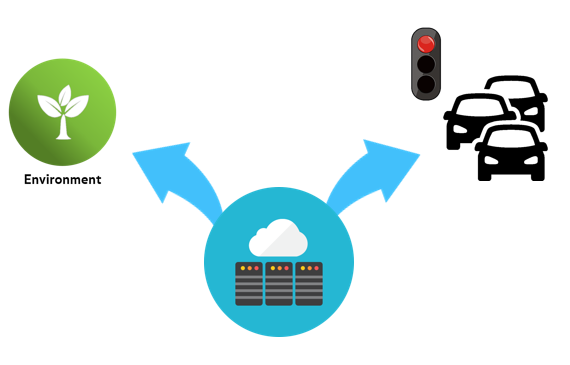
\includegraphics[width=1.0\textwidth]{pic1}
\caption[Mô hình ứng dụng dữ liệu của đề tài]{Mô hình ứng dụng dữ liệu của đề tài}
\label{fig:pic1}
\end{figure}

Và những dữ liệu này có thể ứng dụng cho bất động sản, môi trường và nghiên cứu. Do đó đề tài mang tính thiết thực và ứng dụng cao và được lựa chọn để làm Luận văn tốt nghiệp.




\section{Mục tiêu và nhiệm vụ của đề tài} %Section - 1.1 
\label{section1.2}
\subsection{Mục tiêu đề tài}
\begin{itemize}
\item[-]Tìm hiểu về khí thải xe máy và ô tô.
\item[-]Hiện thực mạch cảm biến để thu thập khí thải.
\item[-]Hiện thực hoàn module thu thập cảm biến tích hợp thêm module sử dụng năng lượng mặt trời để nạp pin cho mạch hoạt động độc lập với điện lưới.
\item[-]Hoàn chỉnh website cho phép người dùng theo dõi thông tin.
\item[-]Đề xuất các tính năng thừa hưởng từ kết quả hệ thống và khả năng tích hợp với các hệ thống khác.
\end{itemize}



\begin{landscape}
\subsection{Nhiệm vụ đề tài}
\begin{table}[]
\centering
\caption{Giản đồ gantt của Huỳnh Phạm So Ny}
\begin{tabular}{|l|l|l|l|l|l|l|l|l|l|l|l|l|l|l|l|l|}
\hline
\multicolumn{1}{|c|}{}                      & \multicolumn{1}{c|}{}                                                                             & \multicolumn{15}{c|}{Tuần}                                                                                                                                                                                                                                                                                                                                                                                                                \\ \cline{3-17} 
\multicolumn{1}{|c|}{\multirow{-2}{*}{STT}} & \multicolumn{1}{c|}{\multirow{-2}{*}{Công việc}}                                                  & 1                        & 2                                               & 3                        & 4                        & 5                        & 6                        & 7                        & 8                        & 9                        & 10                       & 11                       & 12                       & 13                       & 14                       & 15                       \\ \hline
1                                           & \begin{tabular}[c]{@{}l@{}}Tìm hiểu các thiết,bị sensor, MCU, \\ Module SIM\end{tabular}          & \cellcolor[HTML]{000000} & \cellcolor[HTML]{000000}                        & \cellcolor[HTML]{000000} &                          &                          &                          &                          &                          &                          &                          &                          &                          &                          &                          &                          \\ \hline
2                                           & Tìm hiểu về pin,năng lượng mặt trời                                                               &                          & \cellcolor[HTML]{000000}{\color[HTML]{000000} } &                          &                          &                          &                          &                          &                          &                          &                          &                          &                          &                          &                          &                          \\ \hline
3                                           & Làm prototype đầu tiên                                                                            &                          &                                                 &                          & \cellcolor[HTML]{000000} &                          &                          &                          &                          &                          &                          &                          &                          &                          &                          &                          \\ \hline
4                                           & Suy nghĩ design,tổng thể cho cái hộp                                                              &                          &                                                 & \cellcolor[HTML]{000000} & \cellcolor[HTML]{000000} & \cellcolor[HTML]{000000} &                          &                          &                          &                          &                          &                          &                          &                          &                          &                          \\ \hline
5                                           & Thiết kế bản vẽ cho,hộp                                                                           &                          &                                                 &                          &                          &                          & \cellcolor[HTML]{000000} &                          &                          &                          &                          &                          &                          &                          &                          &                          \\ \hline
6                                           & Coding                                                                                            &                          &                                                 &                          &                          &                          & \cellcolor[HTML]{000000} &                          &                          &                          &                          &                          &                          &                          &                          &                          \\ \hline
7                                           & Thiết kế PCB cho,mạch                                                                             &                          &                                                 &                          &                          &                          & \cellcolor[HTML]{000000} & \cellcolor[HTML]{000000} &                          &                          &                          &                          &                          &                          &                          &                          \\ \hline
8                                           & \begin{tabular}[c]{@{}l@{}}Hoàn thiện node cảm biến chạy bằng \\ năng lượng mặt trời\end{tabular} &                          &                                                 &                          &                          &                          &                          & \cellcolor[HTML]{000000} & \cellcolor[HTML]{000000} &                          &                          &                          &                          &                          &                          &                          \\ \hline
9                                           & Testing                                                                                           &                          &                                                 &                          &                          &                          &                          &                          &                          & \cellcolor[HTML]{000000} & \cellcolor[HTML]{000000} & \cellcolor[HTML]{000000} &                          &                          &                          &                          \\ \hline
10                                          & Chọn lại Module SIM và redesign lại PCB                                                           &                          &                                                 &                          &                          &                          &                          &                          &                          &                          &                          & \cellcolor[HTML]{000000} &                          &                          &                          &                          \\ \hline
11                                          & Nhân bản ra 2 node,cảm biến                                                                       &                          &                                                 &                          &                          &                          &                          &                          &                          &                          &                          & \cellcolor[HTML]{000000} & \cellcolor[HTML]{000000} &                          &                          &                          \\ \hline
12                                          & Đi thu thập dữ liệu  \& viết báo cáo                                                              &                          &                                                 &                          &                          &                          &                          &                          &                          &                          &                          &                          &                          & \cellcolor[HTML]{000000} & \cellcolor[HTML]{000000} & \cellcolor[HTML]{000000} \\ \hline
\end{tabular}
\end{table}
\end{landscape}











\begin{landscape}

\begin{table}[]
\centering
\caption{Giản đồ gantt của Nguyễn Mạnh Cường}
\begin{tabular}{|l|l|l|l|l|l|l|l|l|l|l|l|l|l|l|l|l|}
\hline
\multicolumn{1}{|c|}{}                      & \multicolumn{1}{c|}{}                                                                                                 & \multicolumn{15}{c|}{Tuần}                                                                                                                                                                                                                                                                                                                                                                                         \\ \cline{3-17} 
\multicolumn{1}{|c|}{\multirow{-2}{*}{STT}} & \multicolumn{1}{c|}{\multirow{-2}{*}{Công việc}}                                                                      & 1                        & 2                        & 3                        & 4                        & 5                        & 6                        & 7                        & 8                        & 9                        & 10                       & 11                       & 12                       & 13                       & 14                       & 15                       \\ \hline
1                                           & \begin{tabular}[c]{@{}l@{}}Tìm hiểu về web,server, Nodejs, \\ mô hình template cho web\end{tabular}                   & \cellcolor[HTML]{000000} & \cellcolor[HTML]{000000} &                          &                          &                          &                          &                          &                          &                          &                          &                          &                          &                          &                          &                          \\ \hline
2                                           & \begin{tabular}[c]{@{}l@{}}Tìm hiểu high,chart, Json cho \\ việc hiện thực biểu đồ\end{tabular}                       &                          &                          & \cellcolor[HTML]{000000} & \cellcolor[HTML]{000000} &                          &                          &                          &                          &                          &                          &                          &                          &                          &                          &                          \\ \hline
3                                           & \begin{tabular}[c]{@{}l@{}}Hiện thực các chức,năng cho server\\ (google map, add,config Node, graph...)\end{tabular}  &                          &                          &                          & \cellcolor[HTML]{000000} & \cellcolor[HTML]{000000} & \cellcolor[HTML]{000000} & \cellcolor[HTML]{000000} &                          &                          &                          &                          &                          &                          &                          &                          \\ \hline
4                                           & Tìm hiểu về Node,Mailer, hiện thựcsend mail                                                                           &                          &                          &                          &                          &                          &                          & \cellcolor[HTML]{000000} & \cellcolor[HTML]{000000} &                          &                          &                          &                          &                          &                          &                          \\ \hline
5                                           & Tìm hiểu Ionic,framework                                                                                              &                          &                          &                          &                          &                          &                          &                          &                          & \cellcolor[HTML]{000000} & \cellcolor[HTML]{000000} &                          &                          &                          &                          &                          \\ \hline
6                                           & \begin{tabular}[c]{@{}l@{}}Hiện thực giao diện mobile app và \\ một số chức năng, tìm hiểu angular chart\end{tabular} &                          &                          &                          &                          &                          &                          &                          &                          &                          & \cellcolor[HTML]{000000} & \cellcolor[HTML]{000000} & \cellcolor[HTML]{000000} &                          &                          &                          \\ \hline
7                                           & \begin{tabular}[c]{@{}l@{}}Hoàn thiện web,server, sửa lỗi một số \\ chức năng \& viết báo cáo\end{tabular}            &                          &                          &                          &                          &                          &                          &                          &                          &                          &                          &                          &                          & \cellcolor[HTML]{000000} & \cellcolor[HTML]{000000} & \cellcolor[HTML]{000000} \\ \hline
\end{tabular}
\end{table}

\end{landscape}



\begin{landscape}
\begin{table}[]
\centering
\caption{Giản đồ gantt của Võ Tấn Tùng}
\begin{tabular}{|l|l|l|l|l|l|l|l|l|l|l|l|l|l|l|l|l|}
\hline
\multicolumn{1}{|c|}{}                      & \multicolumn{1}{c|}{}                                                                                            & \multicolumn{15}{c|}{Tuần}                                                                                                                                                                                                                                                                                                                                                                                                                                                              \\ \cline{3-17} 
\multicolumn{1}{|c|}{\multirow{-2}{*}{STT}} & \multicolumn{1}{c|}{\multirow{-2}{*}{Công việc}}                                                                 & 1                        & 2                                               & 3                        & 4                        & 5                        & 6                        & 7                                               & 8                        & 9                        & 10                                              & 11                       & 12                       & 13                       & 14                       & 15                       \\ \hline
1                                           & Tìm hiểu về các công cụ hỗ trợ xây dựng server                                                                   & \cellcolor[HTML]{000000} & \cellcolor[HTML]{000000}                        &                          &                          &                          &                          &                                                 &                          &                          &                                                 &                          &                          &                          &                          &                          \\ \hline
2                                           & Tìm hiểu về các công cụ lập trình web                                                                            &                          & \cellcolor[HTML]{000000}{\color[HTML]{FFFFFF} } &                          &                          &                          &                          &                                                 &                          &                          &                                                 &                          &                          &                          &                          &                          \\ \hline
3                                           & Tìm hiểu và lựa chọn Database phù hợp                                                                            &                          & \cellcolor[HTML]{000000}                        & \cellcolor[HTML]{000000} &                          &                          &                          &                                                 &                          &                          &                                                 &                          &                          &                          &                          &                          \\ \hline
4                                           & Thiết kế mô hình hệ thống server                                                                                 &                          &                                                 &                          & \cellcolor[HTML]{000000} & \cellcolor[HTML]{000000} &                          &                                                 &                          &                          &                                                 &                          &                          &                          &                          &                          \\ \hline
5                                           & Khởi tạo Server và Database server                                                                               &                          &                                                 &                          &                          & \cellcolor[HTML]{000000} &                          &                                                 &                          &                          &                                                 &                          &                          &                          &                          &                          \\ \hline
6                                           & Thiết kế APIs và Server URL Routing                                                                              &                          &                                                 &                          &                          &                          & \cellcolor[HTML]{000000} &                                                 &                          &                          &                                                 &                          &                          &                          &                          &                          \\ \hline
7                                           & Hiện thực APIs                                                                                                   &                          &                                                 &                          &                          &                          & \cellcolor[HTML]{000000} & \cellcolor[HTML]{000000}                        &                          &                          &                                                 &                          &                          &                          &                          &                          \\ \hline
8                                           & \begin{tabular}[c]{@{}l@{}}Thử nghiệm tính ổn định APIs \\ với mạch sensor node\end{tabular}                     &                          &                                                 &                          &                          &                          &                          & \cellcolor[HTML]{000000}{\color[HTML]{000000} } &                          &                          &                                                 &                          &                          &                          &                          &                          \\ \hline
9                                           & \begin{tabular}[c]{@{}l@{}}Hiện thực URL Web Routing và nhúng\\ code frontend\end{tabular}                       &                          &                                                 &                          &                          &                          &                          & \cellcolor[HTML]{000000}                        & \cellcolor[HTML]{000000} & \cellcolor[HTML]{000000} &                                                 &                          &                          &                          &                          &                          \\ \hline
10                                          & \begin{tabular}[c]{@{}l@{}}Tìm hiểu và khởi tạo Server chạy \\ trên Raspberry\end{tabular}                       &                          &                                                 &                          &                          &                          &                          &                                                 & \cellcolor[HTML]{000000} &                          &                                                 &                          &                          &                          &                          &                          \\ \hline
11                                          & \begin{tabular}[c]{@{}l@{}}Duyệt lại và chỉnh sửa các đoạn code \\ xung đột và tối ưu code frontend\end{tabular} &                          &                                                 &                          &                          &                          &                          &                                                 &                          & \cellcolor[HTML]{000000} & \cellcolor[HTML]{000000}                        &                          &                          &                          &                          &                          \\ \hline
12                                          & Hiện thực xác thực người dùng                                                                                    &                          &                                                 &                          &                          &                          &                          &                                                 &                          &                          & \cellcolor[HTML]{000000}{\color[HTML]{000000} } & \cellcolor[HTML]{000000} &                          &                          &                          &                          \\ \hline
13                                          & \begin{tabular}[c]{@{}l@{}}Hiện thực cung cấp log và trang log \\ cho nhà phát triển\end{tabular}                &                          &                                                 &                          &                          &                          &                          &                                                 &                          &                          &                                                 & \cellcolor[HTML]{000000} &                          &                          &                          &                          \\ \hline
14                                          & Hiện thực trang thống kê statis                                                                                  &                          &                                                 &                          &                          &                          &                          &                                                 &                          &                          &                                                 &                          & \cellcolor[HTML]{000000} &                          &                          &                          \\ \hline
15                                          & Duyệt và tối ưu hóa code Server                                                                                  &                          &                                                 &                          &                          &                          &                          &                                                 &                          &                          &                                                 &                          & \cellcolor[HTML]{000000} & \cellcolor[HTML]{000000} &                          &                          \\ \hline
16                                          & Đánh giá hệ thống và viết báo cáo                                                                                &                          &                                                 &                          &                          &                          &                          &                                                 &                          &                          &                                                 &                          &                          & \cellcolor[HTML]{000000} & \cellcolor[HTML]{000000} & \cellcolor[HTML]{000000} \\ \hline
\end{tabular}
\end{table}
\end{landscape}


\section{Cấu trúc báo cáo} %Section - 1.1 
Luận văn được chia thành 5 chương, nội dung chính của mỗi chương như sau:

\textbf{Chương 1: Giới thiệu}\\
Giới thiệu sơ bộ về ý tưởng cũng như tính cấp bách, mục tiêu và nhiệm vụ của đề tài và cấu trúc bản báo cáo.

\textbf{Chương 2: Cơ sở lý thuyết}\\
Giới thiệu lý thuyết về các yếu tố ảnh hưởng tới chất lượng môi trường và các hệ thống quan trắc hiện hữu. Bên cạnh đó trình bày kiến thức nền tảng về Internet of Things, các công cụ và thiết bị phần cứng hỗ trợ phát triển IoT được áp dụng thực hiện đề tài. Bên cạnh đó là các khái niệm về các công nghệ, nền tảng xây dựng Server và Database được sử dụng cũng như phát triển ứng dung web và di động cụ thể của hệ thống.

\textbf{Chương 3: Thiết kế}\\
Chương này trình bày thiết kế, cách thức hoạt động của hệ thống, các loại cảm biến được sử dụng và chuẩn giao tiếp được sử dụng.

\textbf{Chương 4: Hiện thực và thử nghiệm}\\
Hiện thực dựa trên bản thiết kế được trình bày, hiện thực các sensor node, hệ thống Server , ứng dụng Web và di động.

Sau khi hiện thực, nhóm thống kê những kết quả thực tế đo được, đánh giá mức độ ổn định của sensor node và server cũng như trải nghiệm ứng dụng web và di động.

\textbf{Chương 5: Tổng kết}\\
Chương này sẽ đút kết những gì đạt được và khó khăn trong việc hiện thực đề tài. Bên cạnh đó đề ra hướng phát triển đề tài trong tương lai.


%*******************************************************************************
%****************************** Second Chapter *********************************
%*******************************************************************************

\chapter{CƠ SỞ LÝ THUYẾT}

\ifpdf
    \graphicspath{{Chapter2/Figs/Raster/}{Chapter2/Figs/PDF/}{Chapter2/Figs/}{Chapter2/Figs/web/}}
\else
    \graphicspath{{Chapter2/Figs/Vector/}{Chapter2/Figs/}}
\fi


%\section[Short title]{Reasonably long section title}
\section{Giới thiệu về Internet of Things và các ứng dụng giám sát}
\subsection{Internet of Things (IoT)}\label{sec:xuhuongiot}
Với sự phát triển nhanh chóng của công nghê máy tính hiện nay, những công nghệ cao đã đang và ngày càng được ứng dụng trong nhiều lĩnh vực của cuộc sống con người. IoT là mạng lưới của các đối tượng vật lý, các thiết bị, các phương tiện và các đối tượng này được nhúng với các thiết bị điện tử, cảm biến, phần mềm điều khiển, và nó có khả năng trao đổi dữ liệu và thao tác với nhau. IoT cho phép các đối tượng được lắng nghe và điều khiển từ xa trên cơ sở hạ tầng mạng hiện có, các hệ thống máy tính có thể thu thập dữ liệu và điều khiển các thiết bị đối tượng một cách hiệu quả, chính xác và lợi ích kinh tế nhất có thể. 
\begin{figure}[H] 
\centering    
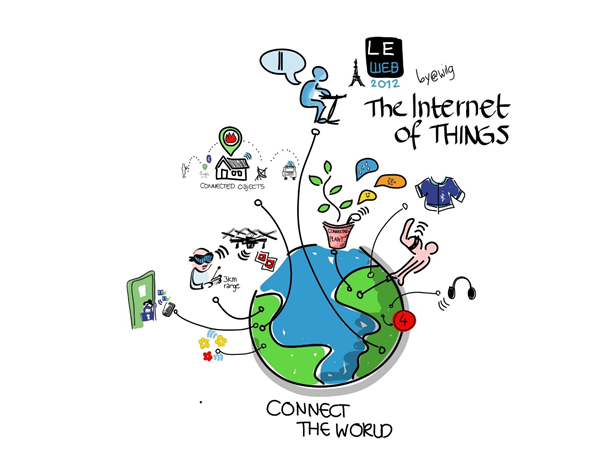
\includegraphics[width=0.7\textwidth]{pic4}
\caption[Hình ảnh mô tả Internet of Things]{Hình ảnh mô tả Internet of Things}
\label{fig:pic4}
\end{figure}


\subsubsection*{Khả năng định danh độc nhất }
Điểm quan trọng của IoT đó là các đối tượng phải có thể được nhận biết và định dạng. Nếu mọi đội tượng, kể cả con người, được "đánh dấu" để phân biệt bản thân đối tượng đó với những thứ xung quanh thì chúng ta có thể hoàn toàn quản lí được nó thông qua máy tính. Việc đánh dấu có thể được thực hiện thông qua nhiều công nghệ, chẳng hạn như RFID, NFC, mã vạch, mã QR, watermark kĩ thuật số... Việc kết nối thì có thể thực hiện qua Wi-Fi, mạng viễn thông băng rộng (3G, 4G), Bluetooth, ZigBee, hồng ngoại...
Ngoài những kĩ thuật nói trên, nếu nhìn từ thế giới web, chúng ta có thể sử dụng các địa chỉ độc nhất để xác định từng vật, chẳng hạn như địa chỉ IP. Mỗi thiết bị sẽ có một IP riêng biệt không nhầm lẫn. Sự xuất hiện của IPv6 với không gian địa chỉ cực kì rộng lớn sẽ giúp mọi thứ có thể dễ dàng kết nối vào Internet cũng như kết nối với nhau.

\subsubsection*{Xu hướng và tính chất của The Internet of Things}
\textbf{Thông minh:} Sự thông minh và tự động trong điều khiển thực chất không phải là một phần trong ý tưởng về IoT. Các máy móc có thể dễ dàng nhận biết và phản hồi lại môi trường xung quanh (ambient intelligence), chúng cũng có thể tự điều khiển bản thân (autonomous control) mà không cần đến kết nối mạng. Tuy nhiên, trong thời gian gần đây người ta bắt đầu nghiên cứu kết hợp hai khái niệm IoT và autonomous control lại với nhau. Tương lai của IoT có thể là một mạng lưới các thực thể thông minh có khả năng tự tổ chức và hoạt động riêng lẻ tùy theo tình huống, môi trường, đồng thời chúng cũng có thể liên lạc với nhau để trao đổi thông tin, dữ liệu.

Việc tích hợp trí thông minh vào IoT còn có thể giúp các thiết bị, máy móc, phần mềm thu thập và phân tích các dấu vết điện tử của con người khi chúng ta tương tác với những thứ thông minh, từ đó phát hiện ra các tri thức mới liên quan tới cuộc sống, môi trường, các mối tương tác xã hội cũng như hành vi con người.

\textbf{Kiến trúc dựa trên sự kiện:} Các thực thể, máy móc trong IoT sẽ phản hồi dựa theo các sự kiện diễn ra trong lúc chúng hoạt động theo thời gian thực. Một số nhà nghiên cứu từng nói rằng một mạng lưới các sensor chính là một thành phần đơn giản của IoT.

\textbf{Là một hệ thống phức tạp:}Trong một thế giới mở, IoT sẽ mang tính chất phức tạp bởi nó bao gồm một lượng lớn các đường liên kết giữa những thiết bị, máy móc, dịch vụ với nhau, ngoài ra còn bởi khả năng thêm vào các nhân tốc mới.

\textbf{Kích thước: } Một mạng lưới IoT có thể chứa đến 50 đến 100 nghìn tỉ đối tượng được kết nối và mạng lưới này có thể theo dõi sự di chuyển của từng đối tượng. Một con người sống trong thành thị có thể bị bao bọc xung quanh bởi 1000 đến 5000 đối tượng có khả năng theo dõi.

\textbf{Vấn đề không gian, thời gian: }Trong IoT, vị trí địa lý chính xác của một vật nào đó là rất quan trọng. Hiện nay, Internet chủ yếu được sử dụng để quản lí thông tin được xử lý bởi con người. Do đó những thông tin như địa điểm, thời gian, không gian của đối tượng không mấy quan trọng bởi người xử lí thông tin có thể quyết định các thông tin này có cần thiết hay không, và nếu cần thì họ có thể bổ sung thêm. Trong khi đó, IoT về lý thuyết sẽ thu thập rất nhiều dữ liệu, trong đó có thể có dữ liệu thừa về địa điểm, và việc xử lí dữ liệu đó được xem như không hiệu quả. Ngoài ra, việc xử lí một khối lượng lớn dữ liệu trong thời gian ngắn đủ để đáp ứng cho hoạt động của các đối tượng cũng là một thác thức hiện nay.

\subsubsection*{Mô hình theo xu hướng IoT thực tế}
\begin{figure}[H]
\centering  
  \begin{subfigure}[b]{0.5\textwidth}
    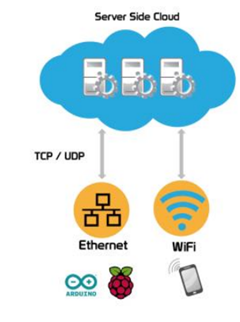
\includegraphics[width=0.8\textwidth]{pic5}
    \caption[Không Gateway]{Không Gateway}
    \label{fig:pic5}
  \end{subfigure}\hfill
  \begin{subfigure}[b]{0.5\textwidth}
    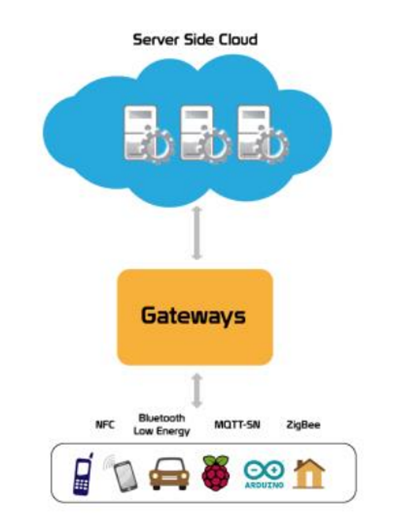
\includegraphics[width=0.8\textwidth]{pic6}
  	 \caption[Có Gateway]{Có Gateway}
    \label{fig:pic6}
  \end{subfigure}
  \caption{Mô hình IoT}\label{fig:mohinhiot}
\end{figure}

Mô hình (Hình ~\ref{fig:pic5}): Các thiết bị sẽ có thể kết nối với nhau bằng TCP/UDP và có thể kết nối trực tiếp đến máy chủ mà không cần thông qua thiết bị khác.\\
Mô hình (Hình ~\ref{fig:pic6}): Các thiết bị sẽ được hỗ trợ nhiều chuẩn giao tiếp khác nhau (BLE, ZWave,…) nên cần cầu nối là Gateway để kết nối đến máy chủ. 

Sơ đồ lớp Chung của cả hai mô hình trên:
\begin{figure}[H] 
\centering    
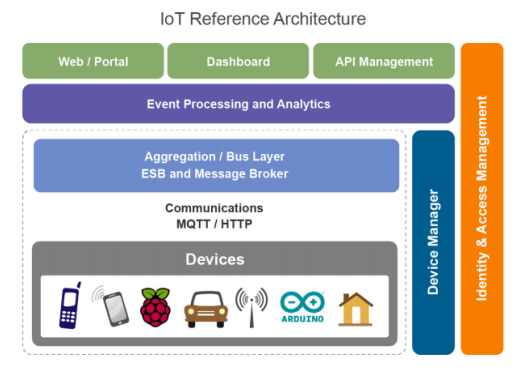
\includegraphics[width=0.8\textwidth]{pic7}
\caption[Kiến trúc mô hình IoT tham khảo]{Kiến trúc mô hình IoT tham khảo}
\label{fig:pic7}
\end{figure}

\begin{itemize}
\item[•]Lớp Device \\
Lớp dưới cùng của kiến trúc là lớp thiết bị. Thiết bị có thể được các loại khác nhau, nhưng để có thể được xem là thiết bị IOT, nó phải có một số thông tin liên lạc hoặc gián tiếp hoặc trực tiếp với Internet.\\
Mỗi thiết bị thường cần một ID. ID có thể là: Bluetooth identifier, Wi-Fi MAC Address…
\item[•]Lớp Communications \\
Các lớp truyền thông hỗ trợ các kết nối của các thiết bị tới máy chủ. Có nhiều giao thức để giao tiếp giữa các thiết bị và máy chủ. Nổi bật nhất là HTTP hoặc MQTT.\\
HTTP rất thông dụng. Bởi vì nó là một giao thức dựa trên văn bản đơn giản, nhiều thiết bị nhỏ như bộ điều khiển 8-bit có thể hỗ trợ một phần các giao thức - ví dụ đủ dữ liệu để POST hoặc GET một nguồn tài nguyên. Các thiết bị lớn hơn 32-bit có thể sử dụng đầy đủ các thư viện HTTP client đúng cách để hiện thực toàn bộ giao thức.\\
MQTT được phát minh vào năm 1999 để giải quyết các vấn đề trong hệ thống nhúng và SCADA. Nó đã được thông qua một số lần lặp lại và phiên bản hiện tại (3.1.1) đang trải qua những tiêu chuẩn hoá trong OASIS MQTT kỹ thuật Committee8. MQTT là một hệ thống tin nhắn publish-subscribe dựa trên một mô hình broker. Các giao thức có một chi phí rất nhỏ (ít nhất là 2 byte cho mỗi tin nhắn). MQTT được thiết kế để vận hành qua TCP.
\item[•]Lớp Aggregation/Bus \\
Một lớp quan trọng của kiến trúc là lớp mà tập hợp và là cầu nối, có khả năng tổng hợp và kết hợp các thông tin liên lạc từ các thiết bị khác nhau và đưa thông tin liên lạc đến một thiết bị cụ thể (có thể thông qua một gateway).
\item[•]Lớp Event Processing and Analytic: \\
Lớp này có các sự kiện từ lớp Bus và cung cấp khả năng xử lý và hành động theo những sự kiện này. Yêu cầu phải lưu trữ các dữ liệu vào một cơ sở dữ liệu nên buộc phải có một ứng dụng ở máy chủ.
\item[•]Lớp External Communications (Top) \\
Lớp này cung cấp một cách cho các thiết bị để chúng giao tiếp ra bên ngoài hệ thống một cách có định hướng và thân thiện với người dùng (Web, Dashboard, API Management)
\end{itemize}

% Please add the following required packages to your document preamble:
Bảng \ref{table:danhgiamohinh} trình bày tổng kết và đánh giá các mô hình trên.
\begin{table}[]
\centering
\caption{So sánh ưu và nhược điểm của các mô hình IoT}
\label{table:danhgiamohinh}
\begin{tabular}{|l|l|l|}
\hline
\textbf{MÔ HÌNH} & \textbf{ƯU ĐIỂM} & \textbf{NHƯỢC ĐIỂM} \\ \hline
\textbf{Mô hình cũ} & Đơn giản hiện thực & \begin{tabular}[c]{@{}l@{}}Gateway cồng kềnh vì phải có \\ bộ phận thu/phát hồng ngoại \\ và các mạch để giao tiếp RF.\end{tabular} \\ \hline
\textbf{Mô hình 1} & \begin{tabular}[c]{@{}l@{}}Không cần thông qua \\ gateway, mọi thông tin \\ thiết bị đều được lưu \\ trên máy chủ.\end{tabular} & \begin{tabular}[c]{@{}l@{}}Hạn chế về phương thức giao\\ tiếp vì chỉ sử dụng TCP/UDP \\ để giao tiếp. Không thể điều khiển\\  thiết bị khi không truy cập được \\ máy chủ.\end{tabular} \\ \hline
\textbf{Mô hình 2} & \begin{tabular}[c]{@{}l@{}}Quản lý thiết bị thông qua\\ gateway làm trung gian, nên\\ các thiết bị có thể tương tác\\ với nhau dễ dàng mà không \\ cần đến máy chủ.\end{tabular} & \begin{tabular}[c]{@{}l@{}}Chi phí cao hơn, hệ thống \\ phức tạp hơn. Độ bảo mật \\ cũng cần được quan tâm hơn.\end{tabular} \\ \hline
\end{tabular}
\end{table}



	
\subsection{Các hệ thống giám sát được phát triển dựa trên IoT}
Khi kết nối một chuỗi khổng lồ các cảm biến (sensor) thu thập dữ liệu, thiết bị và máy móc với nhau, điều quan trọng cần nhận ra là thông tin sẽ được chuyển đổi thành hành động với một tốc độ mà chúng ta chưa từng thấy trước kia. Chúng ta đang tiến đến gần, nếu không phải là đã chạm được vào một thế giới của những khoảng thời gian phản ứng cực nhỏ, phản hồi tức thì với mọi điều kiện biến đổi, và mức độ điều khiển chưa từng có trong việc quản lý tài nguyên và tài sản.

Điểm mấu chốt ở đây là đừng nghĩ hẹp. Internet of Things (IoT) không đơn thuần là mang đến sự tiết kiệm trong các mô hình công nghiệp hiện tại. Nó đảo lộn hoàn toàn những mô hình cũ, tạo ra những sản phẩm và dịch vụ mới. Không có một lĩnh vực nào mà trong đó IoT tạo ra ảnh hưởng đặc biệt lớn nhất; bởi IoT sẽ thay đổi hoàn toàn mọi lĩnh vực một cách không thể tưởng tượng được, bao gồm nông nghiệp, năng lượng, an ninh, quản lý thảm họa, y tế, và đó chỉ là một vài lĩnh vực được nhắc đến.

\subsubsection*{Ứng dụng trong xây dụng }
\begin{figure}[H] 
\centering    

\includegraphics[width=1\textwidth]{pic8}
\caption[Ứng dụng IoT trong xây dựng ]{Ứng dụng IoT trong xây dựng }
\label{fig:pic8}
\end{figure}

Ví dụ: Các công ty xây dựng đã bắt đầu trang bị các silo (hầm chứa đồ) và xe tải có các cảm biến theo dõi mức hàng tồn kho, như là lượng bê tông, và biến đổi nó thông qua platform trên nền điện toán đám mây để gia tăng tốc độ phân phối và đảm bảo một dòng lưu thông vật liệu ổn định. Các ông lớn trong ngành công nghiệp dầu mỏ đã bắt đầu thực thi các công nghệ mobile, cảm biến tới máy móc để dự phòng từ trước cho các tai nạn thông qua các phân tích nhanh chóng và hành động tức thời. Khi các cảm biến phát hiện ra một sự cố như rò rỉ hoặc thất thoát đường ống, công nghệ IoT cho phép các công nhân lập tức xác định vị trí của chúng.

\subsubsection*{Ứng dụng trong năng lượng }

\begin{figure}[H] 
\centering    
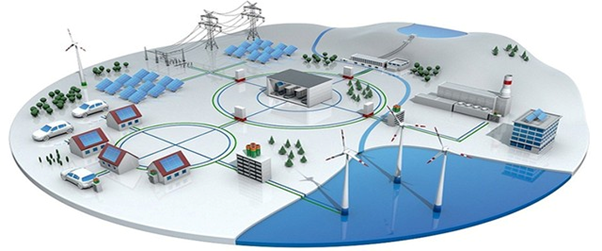
\includegraphics[width=1\textwidth]{pic9}
\caption[Ứng dụng IoT trong năng lượng]{Ứng dụng IoT trongnăng lượng}
\label{fig:pic9}
\end{figure}
Một ví dụ khác của công nghệ IoT mới ứng dụng trong công nghiệp dầu mỏ, đó là giếng thông minh. Đây là một dạng giếng cài đặt các thiết bị điều khiển dòng chảy và cảm biến lỗ khoan, để có thể giám sát và điều khiển từ trên bề mặt mà không đe dọa an toàn của công nhân. Giếng thông minh có trang bị công nghệ địa chấn 4D, cho phép theo dõi sự rò rỉ khí ga, dòng chảy nước, thay đổi áp lực, và bất cứ thay đổi nào khác gây ra bởi những biến động địa chấn, giúp cho việc dự đoán và điều khiển các tác động địa chấn có thể gây ra những hỏng hóc nghiêm trọng.

Nhưng như thế, chúng ta vẫn nghĩ quá hẹp. Hãy vượt ra khỏi lĩnh vực xây dựng hay năng lượng. Chúng ta có các cảm biến có thể đo lực, tải, moment, và áp lực; các cảm biến có thể ngửi thấy mùi khí ga hay hóa chất; những cảm biến có thể nghe thấy rung động và phân biệt giữa các âm hưởng khác nhau; những cảm biến có thể đo nhiệt độ, phát hiện chuyển động, vận tốc và chuyển vị; xác định vị trí, sự có mặt, và khoảng cách. Nói cách khác, chúng ta có khả năng thu thập những hiểu biết gần như không giới hạn, trong thời gian thực.

\subsubsection*{Ứng dụng trong dân dụng  }

\begin{figure}[H] 
\centering    
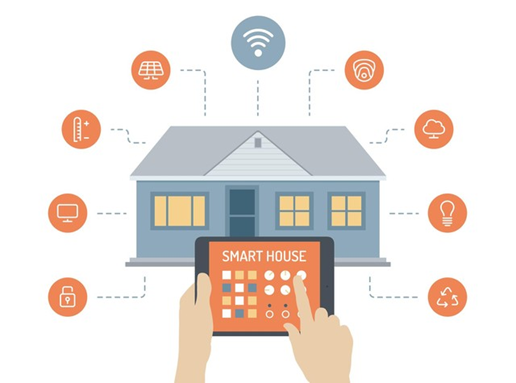
\includegraphics[width=1\textwidth]{pic10}
\caption[Ứng dụng IoT trong dân dụng ]{Ứng dụng IoT trong dân dụng}
\label{fig:pic10}
\end{figure}

Làm thế nào chúng ta có thể tận dụng thông tin thời gian thực từ rất nhiều sensor? Hãy nhìn vào ngôi nhà của chúng ta. Những phần nào trong đó có thể thông minh hóa? Ví dụ đơn giản. Tôi từng quan sát 1 hệ thống video conference cho phép người chủ nói chuyện với chú cún của mình, gọi nó đến, cho nó ăn từ xa thông qua một thiết bị thông minh. Hãy nghĩ lớn hơn nữa. Một ngôi nhà biết khi nào bạn về nhà bởi nó kết nối với một cảm biến trên xe hay smartphone của bạn. Một ngôi nhà kết nối các cảm biến báo khói, hệ thống an ninh, và thiết bị giải trí tới điện thoại của bạn. Một ngôi nhà với các cảm biến được gắn vào đường ống để có thể phát hiện ra rò rỉ trước cả khi điều đó thực sự diễn ra.

\subsubsection*{Ứng dụng trong y tế}
\begin{figure}[H] 
\centering    
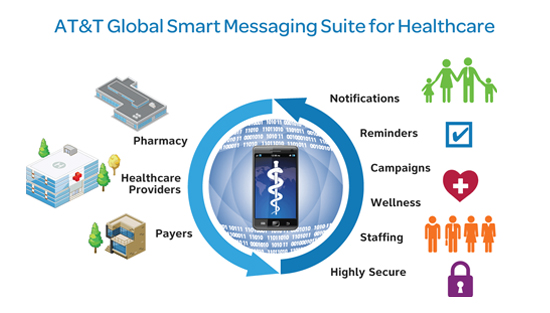
\includegraphics[width=1\textwidth]{pic11}
\caption[Ứng dụng IoT trong y tế ]{Ứng dụng IoT trong y tế}
\label{fig:pic11}
\end{figure}
Công nghệ thiết bị đeo cũng sẽ biến đổi hoàn toàn lĩnh vực chăm sóc sức khỏe theo những cách phi thường. Chúng ta đều biết rằng đồng hộ Apple Watch sẽ tích hợp một cảm biến theo dõi nhịp tim và cung cấp cho chủ của nó những ứng dụng tạo điều kiện và khuyến khích một cách sống lành mạnh. Chúng ta đã có các cảm biến gắn trong giày để theo dõi việc chạy xa đến đâu và bao nhiêu calo đã được đốt. Còn gì tiếp theo? Sẽ có một quy trình tối ưu chăm sóc sức khỏe, theo đó có những cảm biến có thể phát hiện vi khuẩn trong thiết bị, và thiết bị diệt khuẩn phát hiện virus có thể di chuyển từ bệnh nhân.
\subsection{Các ràng buộc của hệ thống}
Cũng như các dự án IoT quy mô rộng khác, đề tài cũng yêu cầu nhiều đặc tính ràng buộc như:  
\subsubsection*{Tính đáp ứng thời gian thực}Để giải quyết tình trạng giao thông hiện thời và trong thời gian gần, ta cần phải có dữ liệu thời gian thực. Ta không thể sử dụng dữ liệu của nửa tiếng hoặc 1 giờ trước để vẽ nên bản đồ lưu thông hiện tại cũng như cách điều hướng giải quyết. Do đó, hệ thống cần phải có thời gian đáp ứng nhanh khi có yêu cầu dữ liệu khi được gọi. Để đạt được kết quả đó, ta cần phải có những phần cứng với thiết lập kết nối có khả năng đáp ứng nhanh, cùng với khả năng hoạt động ổn định liên tục trong thời gian dài để cung cấp dữ liệu liên tục và liền mạch.


\subsubsection*{Toàn vẹn dữ liệu (Data Integrity)} Mục đích chính của dự án là thu thập dữ liệu và từ đó phát triển ứng dụng. Vì thế tính toàn vẹn dữ liệu đóng vai trò quan trọng. Dữ liệu thu thập cần phải đáp ứng đủ các yếu tố: tin cậy, chính xác và đầy đủ. Ta cần phải có đủ dữ liệu thì mới có thể đủ dữ kiện để giải quyết bài toán. Ta không thể giải quyết khi chỉ có được dữ liệu một đoạn đường, 1 thời gian ngắn mà đòi hỏi phải có dữ liệu của một khu vực đủ lớn và tương quan với nhau. Bên cạnh đó cần phải có tính chính xác dữ liệu và đòi hỏi sự ổn định của lượng dữ liệu đó qua yếu tố độ tin cậy. 

\begin{figure}[H]
	\centering    
	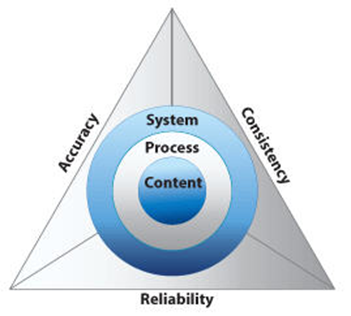
\includegraphics[width=3in]{toanvendulieu}
	\caption[Toàn ven dữ liệu]{Toàn ven dữ liệu}
	\label{fig:toanvendulieu}
\end{figure}

\subsubsection*{Đồng bộ hóa} Hệ thống giám sát môi trường có nhiều thiết thiết bị khác nhau, nhiều phương pháp và cách thức truyền dữ liệu khác nhau. Do đó ta cần phải có sự chuẩn hóa các giao thức giao tiếp, đồng bộ các gói dữ liệu. Tuy nhiên điều này sẽ dẫn đến vấn nạn được đề cập ở mục sau.

\subsubsection*{Tính bảo mật} Vấn đề bảo mật và an toàn dữ liệu hiện tại vẫn là một trong những khó khăn mà hệ thống IoT đang mắc phải. Vì hệ thống IoT đòi hỏi cần phải có giao thức kết nối giữa các thiết bị phải được chuẩn hóa và động bộ, cũng như tối giản kích thước gói tin để tối ưu trong việc truyền dữ liệu giữa các thiết bị, do đó gói tin truyền đi có thiết lập cấu trúc đơn giản và hệ thống dễ bị thâm nhập. Điều này sẽ dẫn đến hệ thống có thể bị đánh cắp dữ liệu, và thậm chí mất quyền kiểm soát toàn bộ hệ thống bởi vì tất cả đều được kết nối với nhau. Vậy nên cần phải cân nhắc trade-off giữa hiệu năng hệ thống và tính bảo mật.
\begin{figure}[H]
	\centering    
	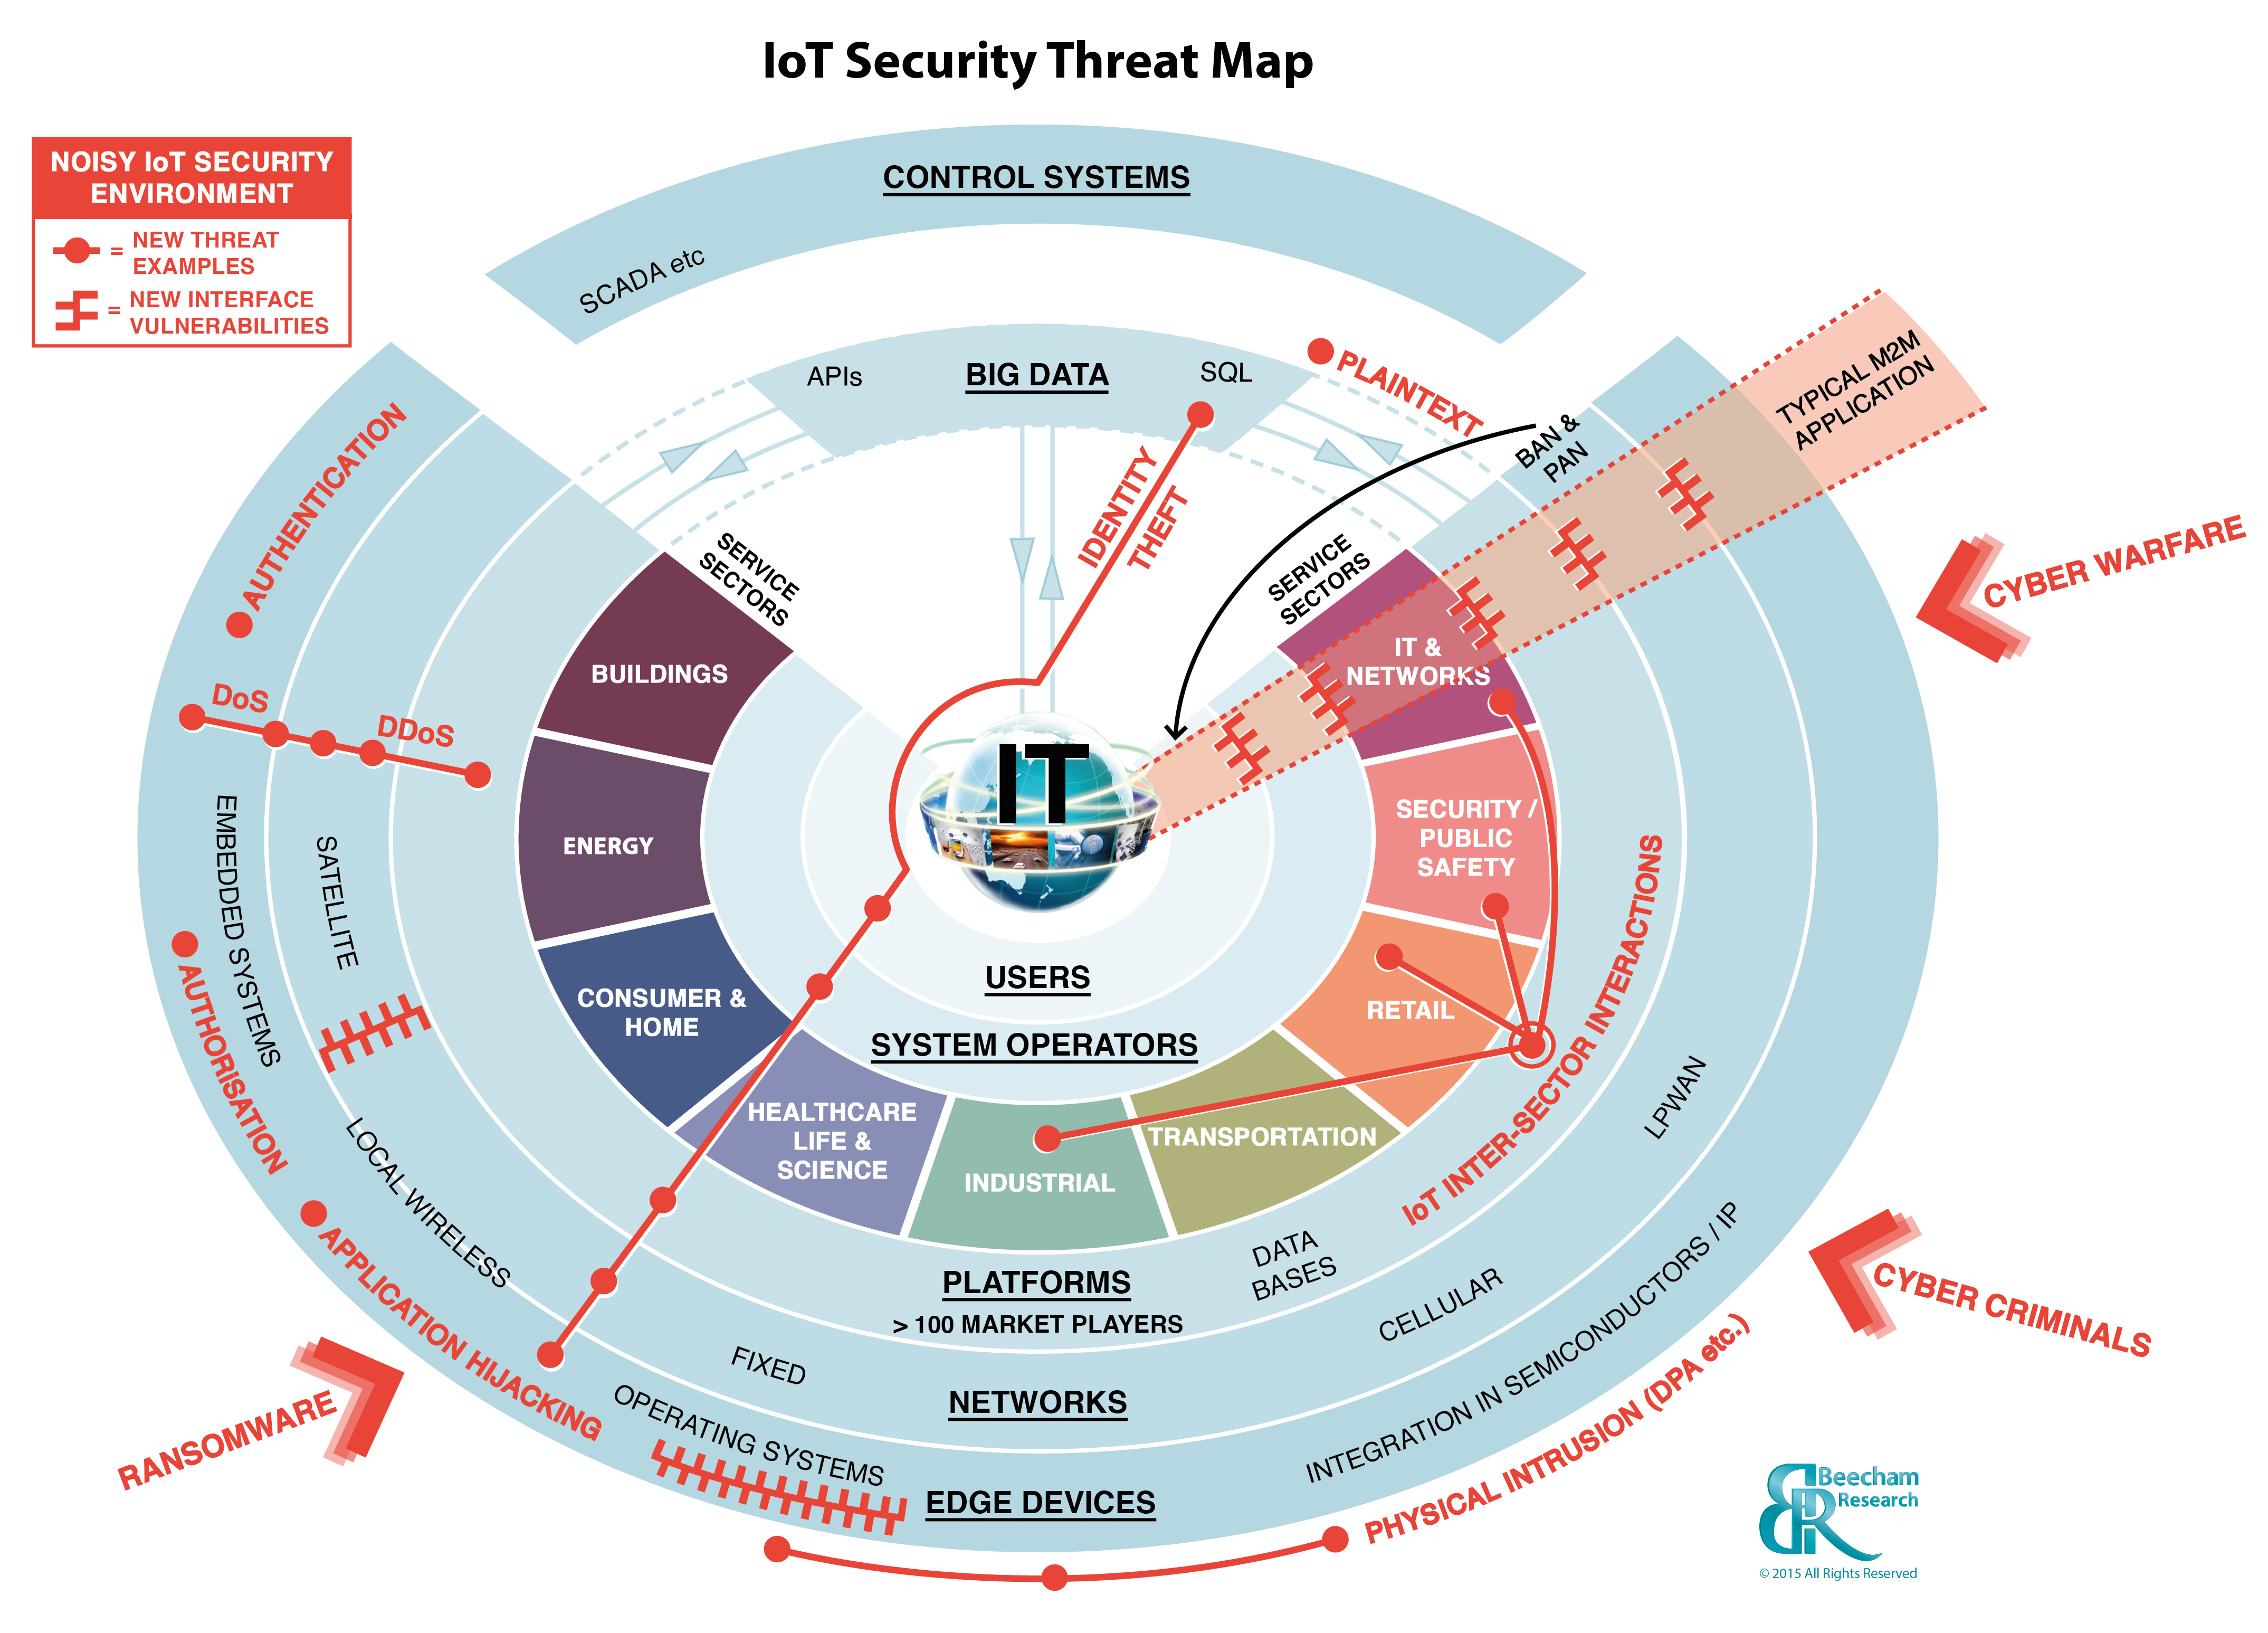
\includegraphics[width=5in]{virusiot}
	\caption[Tính bảo mật]{Tính bảo mật}
	\label{fig:virusiot}
\end{figure}

Các mối nguy hại chính ảnh hưởng trực tiếp tới hệ thống IoT như: DDoS, Ransomware, Cyber Criminals và Cyber Warfare. 




\section{Những yếu tố ảnh hưởng môi trường từ khí thải phương tiện giao thông}\label{sec:yeuto_khithai}
Để hình dung được những yếu tố ảnh hưởng môi trường từ khí thải xe máy và ô tô thì chúng ta cần biết được quá trình hoạt động của xe máy và ô tô, từ đó chúng ta sẽ biết được những loại khí thải nào mà xe máy và ô tô sẽ thải ra môi trường. Qua quá trình tìm hiểu và đọc thông tin tài liệu trên mạng khí thải của xe máy và ô tô tuỳ thuộc chủ yếu vào chất lượng đốt cháy hỗn hợp xăng và không khí bên trong buồng đốt (combustion chamber) của động cơ, cũng như nồng độ các chất ô nhiễm trong khí xả phụ thuộc vào đặc điểm động cơ cũng như các thông số điều chỉnh, vận hành.

Động cơ mới và được điều chỉnh đúng cho phản ứng cháy hoàn chỉnh (complete combustion) hay phản ứng cháy thừa oxy:

\begin{center}
PTPU: Xăng + Không khí → Carbon Dioxide + Nước + Nitrogen
\end{center} 
Các phó sản (by-product) chủ yếu của phản ứng này là nước (H2O) và carbon dioxide (CO2), do đó ống thoát khí cháy (tail pipe) của một động cơ tốt thường có nước nhễu ra, dễ nhận thấy khi động cơ đang trong quá trình làm nóng máy (warm up).

Động cơ cũ hoặc không được điều chỉnh đúng cho phản ứng cháy không hoàn chỉnh (incomplete combustion) hay thiếu oxy:
\begin{center}
PTPU: Xăng + Không khí → Hydrocarbons + Nitrogen Oxides + Carbon Dioxide + Carbon Monoxide + Nước
\end{center}

Phản ứng này tạo thêm những phó sản như carbon monoxide (CO) và nitrogen oxides (NOx). Vậy chúng ta có các loại sản pham như sau:
\begin{itemize}
\item[•]CO được sinh ra khi lượng oxy đưa vào buồng đốt không đủ.
\item[•]HC được sinh ra trong quá trình đốt cháy không hoàn toàn, cũng như CO.
\item[•]NOx được sinh ra do nitơ và ôxy trong hỗn hợp không khí-nhiên liệu, khi nhiệt độ của buồng đốt tăng cao trên 1800oC. Nhiệt độ của buồng đốt càng cao, lượng NOx sản ra càng nhiều.
\end{itemize}
 
 Theo lý thuyết, khi đốt cháy xăng thì chỉ sinh ra CO2 (cácbon điôxit) và H2O (hơi nước). Tuy nhiên, không phải toàn bộ xăng đều tham gia phản ứng như lí thuyết, do ảnh hưởng của các yếu tố như tỷ lệ hỗn hợp không khí-nhiên liệu, nitơ trong không khí, nhiệt độ cháy, thời gian cháy... Đó là nguyên nhân sinh ra các khí độc hại như CO, HC hoặc NOx.
 
Trên cơ sở thực tế, động cơ đốt trong nó chỉ sử dụng được khoảng 30-45\% nhiệt lượng để sinh công, phần còn lại bị hao hụt đi mất, do đó nó mang theo nhiệt lượng thải ra ngoài. Lượng nhiệt này thực tế đã tác động đến môi trường, làm cho nhiệt độ xung quanh những khu vực có xe máy và ô tô tăng lên. Việc đi lại trên những đoạn đường đông xe máy và ô tô thường gây cho chúng ta cảm giác nóng bức, và khó thở. Đó chính là những yếu tố khí thải đã trình bày như trên của xe máy và ô tô đã tác động đến môi trường.

Một phần nhân tố cũng đáng chú ý trong quá trình hoạt động xe máy và ô tô hoạt động đó là bụi, vì đầu vào của động cơ là xăng và không khí, mà trong xăng hiện nay thường có cặn và lượng không khí đầu vào cũng có bụi mặc dù có bộ lọc khí nhưng không thể tránh được trong quá trình sử dụng lâu dài. Một số loại phương tiện giao thông sử dụng thời gian dài, không đi bảo trì sẽ thải ra một nồng độ ô nhiễm rất lớn.

Từ những cơ sơ lý thuyết trên cho chúng ta biết được những yếu tố ảnh hưởng môi trường từ khí thải xe máy và ô tô bao gồm:
\begin{itemize}
\item[•]Khí CO2, CO, HC, NOx.
\item[•]Khói bụi.
\item[•]Yếu tố về nhiệt.
\end{itemize}








\section{Các hệ thống quan trắc hiện hữu}
\subsection{VoV giao thông}
Sử dụng hệ thống camera an ninh kết hợp với lượng phóng viên thường trực khắp thành phố để giám sát trực tiếp và cảnh báo tình trạng lưu thông trên các đoạn đường. Hệ thống có tính hiệu quả rất cao vì sử dụng CCTV giám sát tình trạng giao thông theo thời gian thực nên có góc nhìn thực tế nhất và không phục thuộc, có thể hoạt động độc lập. Tuy nhiên hệ thống vẫn có nhiều hạn chế như:
\begin{itemize}
\item[•]Vẫn chủ yếu hoạt động một cách thủ công, điều tiết và đưa ra kết quả bởi con người, chưa có áp dụng thuật toán xử lý máy tính vào công việc nhiều.
\item[•]Tốn nhiều công sức và nhân lực, cần có nhiều phóng viên trực thuộc các đoạn đường cũng như người quản lý theo dõi hệ thống camera giao thông.
\item[•]Chi phí duy trì và lắp đặt còn khá cao, và cần tốn chi phí bảo trì đắt đỏ và trình độ chuyên môn nhân viên điều hành cao, chi phí một hệ thống có thể lên tới hàng trăm tỉ. Cụ thể như hệ thống trị giá 270 tỉ VNĐ bao gồm 19 trạm giám sát camera được triển khai ở Bà Rịa - Vũng Tàu.
\end{itemize}
\begin{figure}[H] 
\centering    
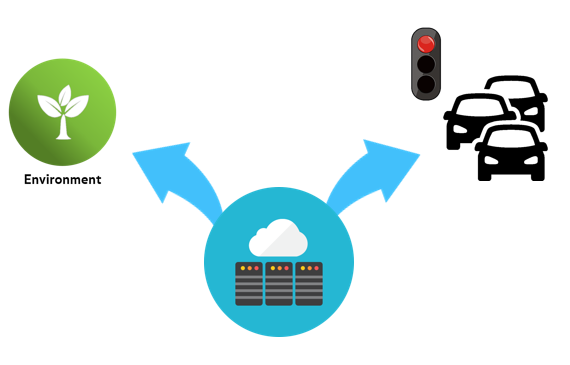
\includegraphics[width=1.0\textwidth]{pic1}
\caption[Trạm giám sát VOV Giao thông ]{Trạm giám sát VOV Giao thông}
\label{fig:pic1}
\end{figure}



\subsection{BKTraffic}
Bktraffic \url{http://traffic.hcmut.edu.vn} kết hợp hệ thống xe bus cùng với định vị GPS và gửi dữ liệu qua hạ tầng mạng 3G để theo dõi vị trí xe và tính toán tốc độ lưu thông trên đoạn đường xe đang lưu thông. Dự án này có hiệu quả cao vì hệ thống xe bus dày đặc và có thời gian hoạt động rộng. Tuy nhiên vẫn có những hạn chế như:
\begin{itemize}
\item[•]Vì chỉ giám sát trên xe bus nhưng nhiều trường hợp không hiệu quả khi áp dụng cho giao thông tại Việt Nam. Bởi vì đa số phương tiện giao thông ở Việt Nam là xe 2 bánh, do đó hệ thống bus di chuyển không phản ảnh được tình trạng lưu thông chung trên tuyến đường đó.
\item[•]Nhiều tuyến đường trên địa bàn thành phố mà xe bus vẫn chưa hoạt động, do vậy vẫn chưa có đủ dữ liệu cần thiết để.
\item[•]Mang tính phụ thuộc vào xe bus, vậy nên có sẽ có những trường hợp ảnh hưởng bởi hệ thống xe bus mà hệ thống sẽ không hoạt động hiệu quả được.
\end{itemize}

\begin{figure}[H] 
\centering    
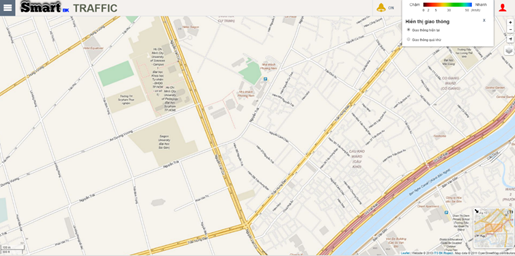
\includegraphics[width=1.0\textwidth]{pic2}
\caption[Ứng dụng Web SmartBKTraffic ]{ Ứng dụng Web SmartBKTraffic}
\label{fig:pic2}
\end{figure}

\subsection{Hệ thống quan trắc môi trường ở Hà Nội}
Thủ đô Hà Nội vừa lắp đặt hệ thống 80 trạm quan trắc. Hệ thống này có tính tương đồng với đề tài đang thực hiện. Tuy nhiên mục đích chính là để theo dõi môi trường sau sự cố bụi Thủy ngân và chưa thấy hướng ứng dụng vào hệ thống giao thông. Hơn nữa, các trạm này chiếm diện tích lắp đặt nên hạn chế khả năng triển khai số lượng lớn trên diện rộng.
\begin{figure}[H] 
\centering    
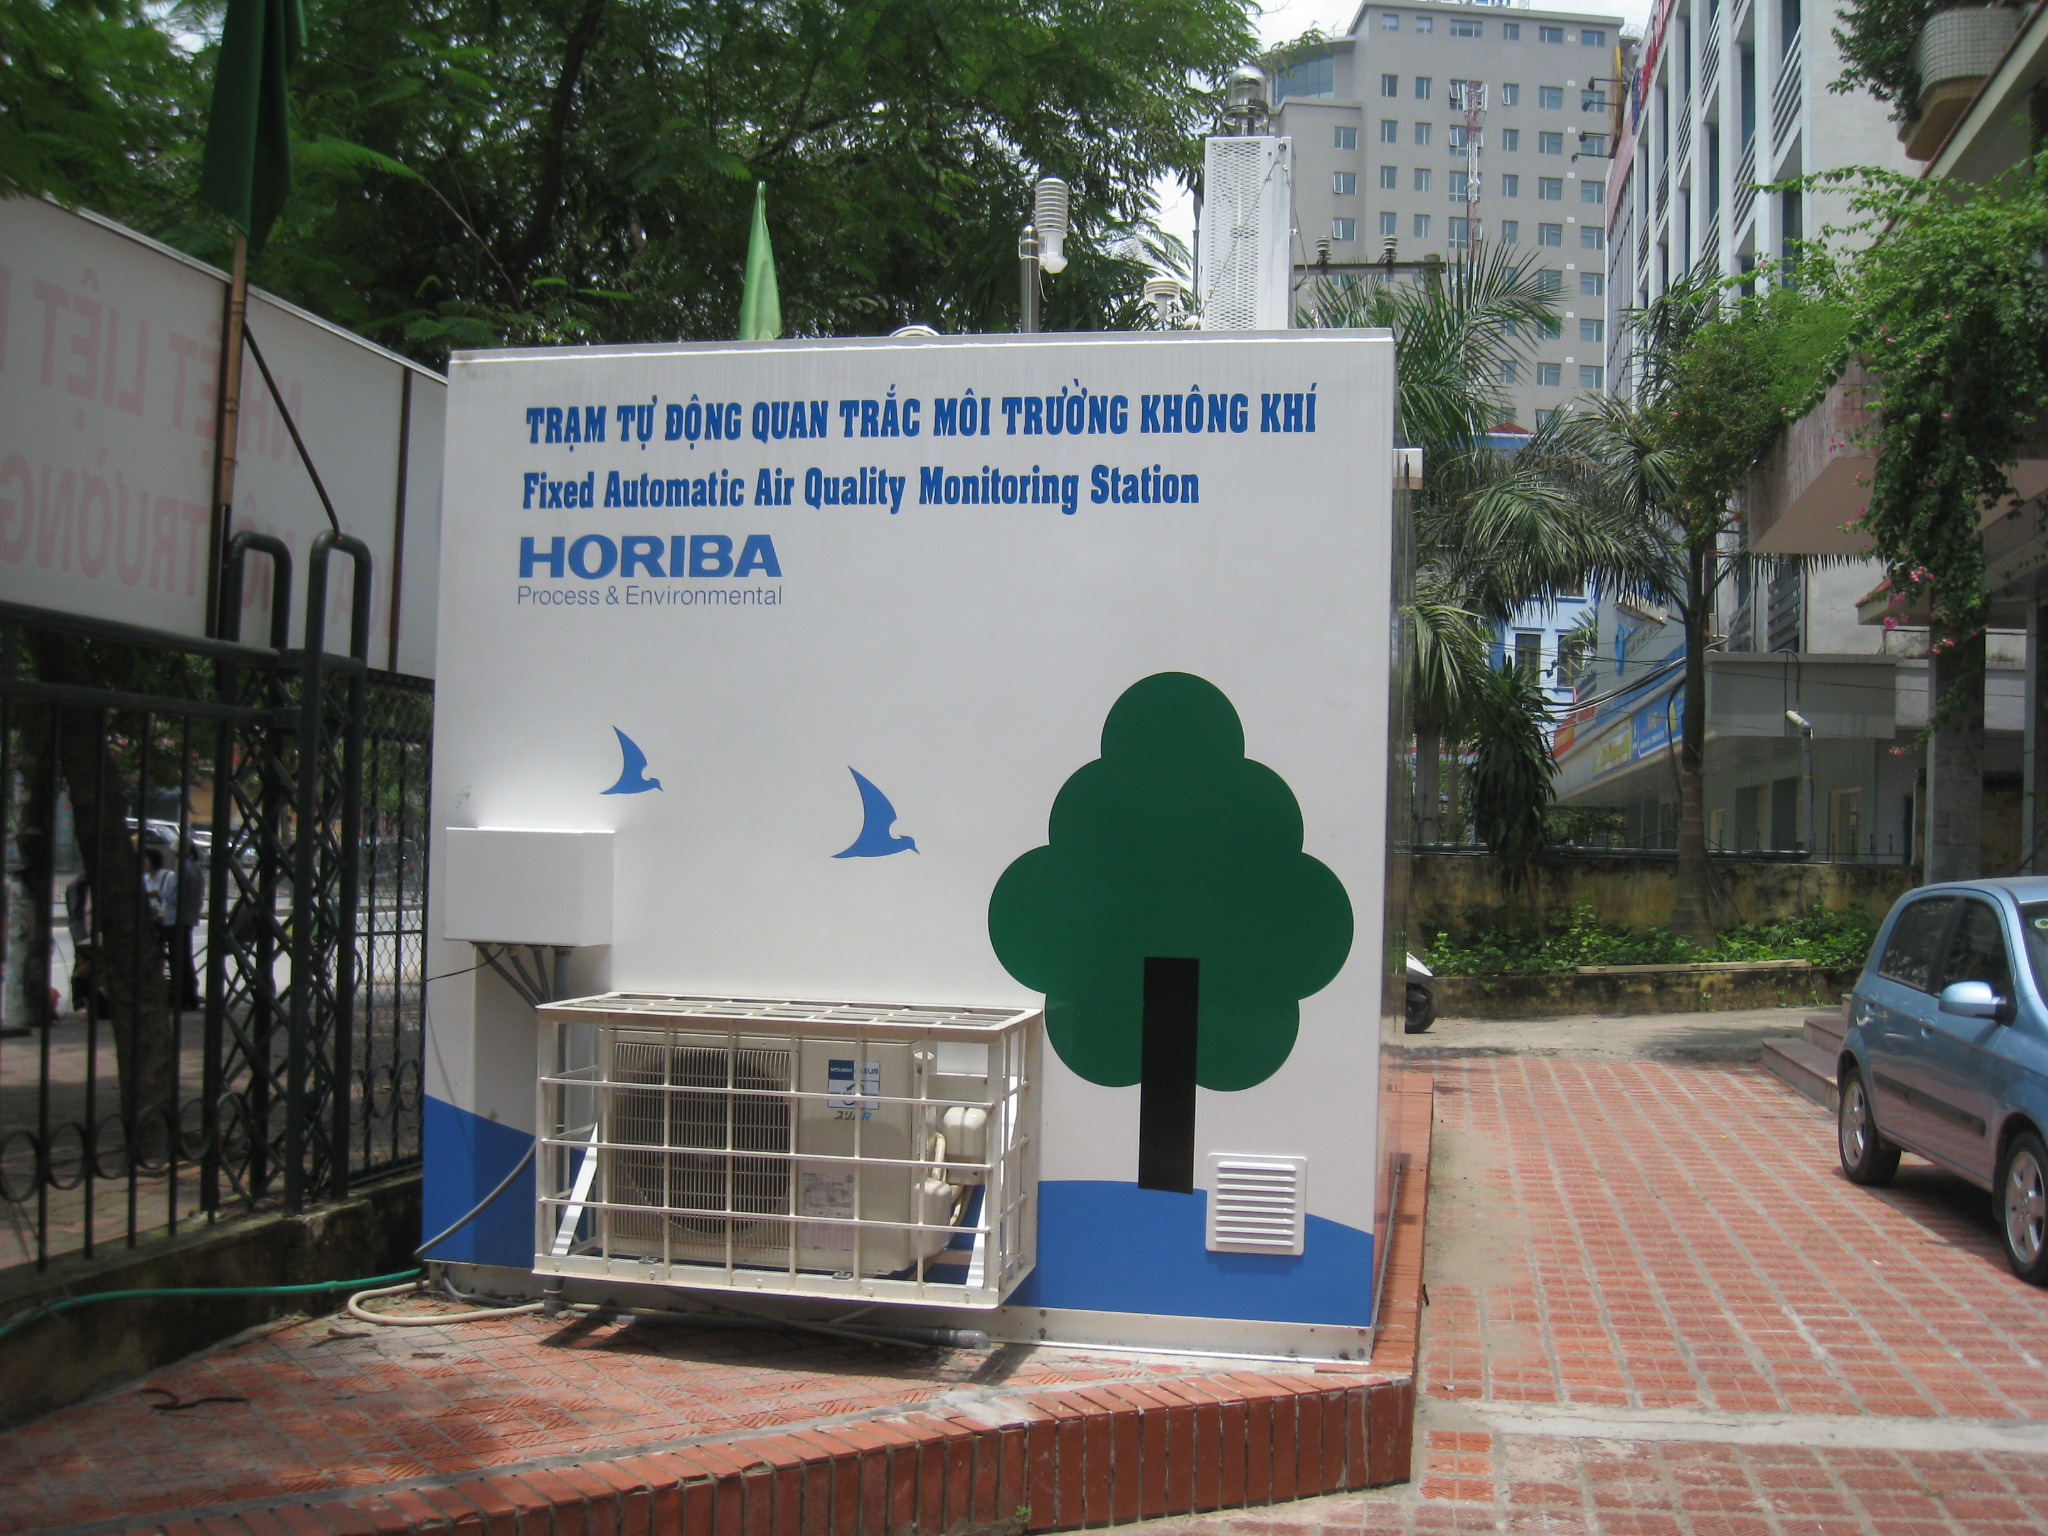
\includegraphics[width=1.0\textwidth]{pic3}
\caption[Trạm quan trắc môi trường tại Hà Nội ]{Trạm quan trắc môi trường tại Hà Nội}
\label{fig:pic3}
\end{figure}

\section{Mô hình quan trắc xây dựng ở giai đoạn Thực tập tốt nghiệp}

%TODO: copy bên báo cáo cũ, sử dụng có gateway

\subsection{Ưu điểm}
\begin{itemize}
	\item[•] Phát triển theo mô hình IoT có sử dụng gateway giúp việc quản lý các node hiệu quả và dễ dàng hơn khi số lượng node lớn.
	\item[•] Có kết quả thực tế biểu hiện được tình trạng giao thông tại thời điểm đó và đủ tin cậy để tham khảo.
	\item[•] Xây dựng mạng lưới liên kết trao đổi thông tin giữa các thiết bị với nhau.
\end{itemize}
\subsection{Nhược điểm}
\begin{itemize}
	\item[•] Khó triển khai được ở điều kiện thực tế tại Việt Nam. Chỉ có thể triển khai dưới sự chấp thuận và quản lý của các cơ quan chức năng.
	\item[•] Yêu cầu lượng dữ liệu đủ lớn mới có thể phân tích được tình trạng giao thông.
	\item[•] Module Zigbee bị giới hạn khoảng cách và độ ổn định giảm đáng kể tại môi trường đường phố tại Việt Nam, làm việc triển khai hoạt động gặp nhiều khó khăn.
\end{itemize}
\section{Các thiết bị phần cứng hỗ trợ cho đề tài}
\subsection{Mạch vi xử lý Arduino}
\subsubsection*{Giới thiệu về Arduino Nano}
Arduino là một board mạch vi xử lý, nhằm xây dựng các ứng dụng tương tác với nhau hoặc với môi trường được thuận lợi hơn. Phần cứng bao gồm một board mạch nguồn mở được thiết kế trên nền tảng vi xử lý AVR Atmel 8bit, hoặc ARM Atmel 32-bit. Những Model hiện tại được trang bị gồm 1 cổng giao tiếp USB, 6 chân đầu vào analog, 14 chân I/O kỹ thuật số tương thích với nhiều board mở rộng khác nhau. Đi cùng với nó là một môi trường phát triển tích hợp (IDE) chạy trên các máy tính cá nhân thông thường và cho phép người dùng viết các chương trình cho Aduino bằng ngôn ngữ C hoặc C++.

\begin{figure}[H]
\centering    
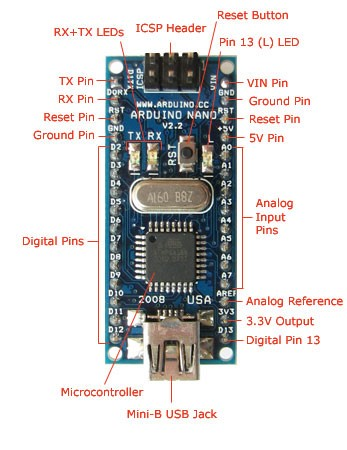
\includegraphics[width=0.4\textwidth]{arduinonano}
\caption[Mạch vi xử lý Arduino Nano]{Mạch vi xử lý Arduino Nano}
\label{fig:arduinonano}
\end{figure}

\begin{center}
\begin{table}[]
\centering
\caption{Thông số của Vi xử lý Arduino}
\label{table:thongsoarduino}
\begin{tabular}{|l|l|}
\hline
Vi điều khiển                 & ATmega328 (họ 8bit)                           \\ \hline
Điện áp hoạt động             & 5VDC                                          \\ \hline
Tần số hoạt động              & 16 MHz                                        \\ \hline
Dòng tiêu thụ                 & 30mA                                          \\ \hline
Điện áp vào khuyên dùng       & 7-12 VDC                                      \\ \hline
Điện áp vào giới hạn          & 6-20 VDC                                      \\ \hline
Số chân Digital I/O           & 14 (6 chân PWM)                               \\ \hline
Số chân Analog                & 8 (độ phân giải 10bit)                        \\ \hline
Dòng,tối đa trên mỗi chân I/O & 40 mA                                         \\ \hline
Dòng ra tối đa (5V)           & 500 mA                                        \\ \hline
Dòng ra tối đa (3.3V)         & 50 mA                                         \\ \hline
Bộ nhớ flash                  & 32 KB (ATmega328) với 2KB dùng bởi bootloader \\ \hline
SRAM                          & 2 KB (ATmega328)                              \\ \hline
EEPROM                        & 1 KB (ATmega328)                              \\ \hline
Kích thước                    & 1.85cm x 4.3cm                                \\ \hline
\end{tabular}
\end{table}
\end{center}


\subsubsection*{Lập trình cho Arduino Nano}
Arduino Nano sử dụng chương trình Arduino IDE để lập trình, và ngôn ngữ lập trình cho Arduino cũng tên là Arduino (được xây dựng trên ngôn ngữ C). 

Arduino IDE là môi trường phát triển tích hợp (IDE) của Arduino là một ứng dụng cross-platform (nền tảng) được viết bằng Java, và từ IDE này sẽ được sử dụng cho ngôn ngữ lập trình xử lý (Processing programming language) và project Wiring. Nó được thiết kế để dành cho những người mới tập tành làm quen với lĩnh vực phát triển phần mềm. Nó bao gồm một chương trình code editor với các chức năng như đánh dấu cú pháp, tự động brace matching, và tự động canh lề, cũng như compile và upload chương trình lên board chỉ với 1 cú click chuột. Một chương trình hoặc code viết cho Arduino được gọi là một sketch.

\begin{figure}[H]
\centering    
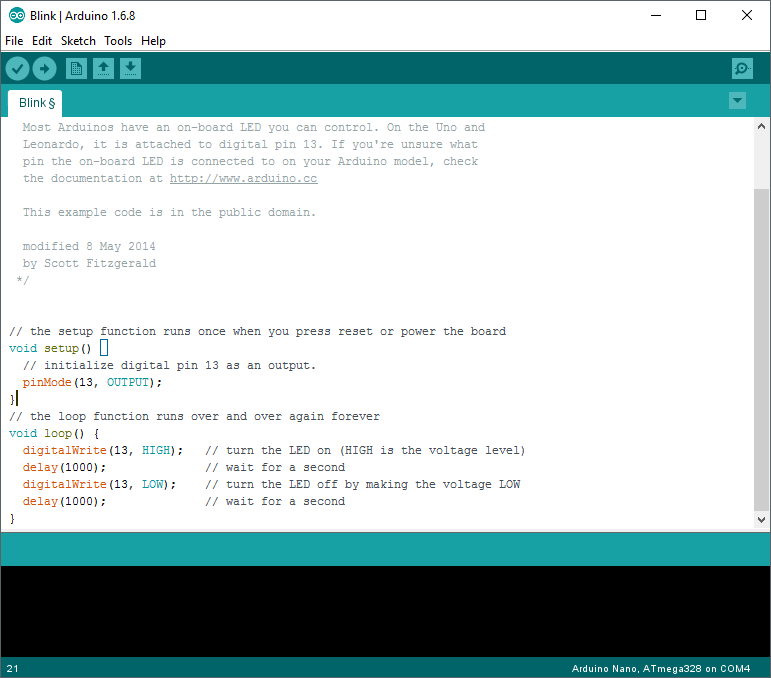
\includegraphics[width=0.7\textwidth]{arduinonano_ide}
\caption[Môi trường phát triển của Arduino]{Môi trường phát triển của Arduino}
\label{fig:arduinonano_ide}
\end{figure}

Các chương trình Arduino được viết bằng C hoặc C++. Arduino IDE đi kèm với một thư viện phần mềm được gọi là "Wiring", từ project Wiring gốc, có thể giúp các thao tác input/output được dễ dàng hơn. Người dùng chỉ cần định nghĩa 2 hàm để tạo ra một chương trình vòng thực thi (cyclic executive) có thể chạy được:
\begin{itemize}
\item[•]Setup(): hàm này chạy mỗi khi khởi động một chương trình, dùng để thiết lập
các cài đặt
\item[•]Loop(): hàm này được gọi lặp lại cho đến khi tắt nguồn board mạch
\end{itemize}

Đoạn code nháy đèn căn bản:
\begin{lstlisting}[numbers=left,firstnumber=1,language=C]
// the setup function runs once
void setup() {
  // initialize digital pin 13 as an output.
  pinMode(13, OUTPUT);
}

// the loop function runs forever
void loop() {
  // turn the LED on (HIGH is the voltage level)
  digitalWrite(13, HIGH);   
  // wait for a second
  delay(1000);    
  // turn the LED off by making the voltage LOW          
  digitalWrite(13, LOW);    
  // wait for a second
  delay(1000);              
}

	\end{lstlisting}







%\\\\\\\\\\\\\\\\\\\\\\\\\\\\\\\\\\\\\\	SIM800L	\\\\\\\\\\\\\\\\\\\\\\\\\\\\\\\\\\\\\\\\\\\\%
\subsection{Module SIM800L}\label{sec:sim800l}
\subsubsection*{Giới thiệu về Sim800L}
Thừa kế các chức năng từ các thế hệ modile sim trước như sim900, Module GSM sim 800L có khả năng nhắn tin SMS, nghe gọi, GPRS, … như một điện thoại nhưng có kích thuốc nhỏ nhất trong các loại module SIM (25 mm x 22 mm). Điều khiển module sử dụng các bộ tập lệnh AT dễ dàng, chân kết nối dùng rào đực thông dụng chuẩn 100mil.
Thông số kỹ thuật:
\begin{itemize}

\item[•]Nguồn cấp: 3.7 – 4.2 VDC, có thể sử dụng với nguồn dòng thấp từ 500mAh trở lên, nhưng để sim hoạt động đảm bảo thì dòng đủ 1A là được khuyến khích dùng hơn.
\item[•]Khe cắm SIM: MICROSIM
\item[•]Dòng khi ở chế độ chờ: 10mA
\item[•]Dòng khi hoạt động: 100mA đến 1A
\item[•]Hỗ trợ 4 băng tần phổ biến: GSM 850, EGSM 900, DCS 1800, PCS 1900.
\item[•]Nhiệt độ hoạt động: -40 C ~ 85 C
\item[•]Tốc độ truyền downlink/uplink: cao nhất 85.6 kbps
\item[•]Tốc độ UART hỗ trợ: 1200bps đến 125200bps
\end{itemize}

Chức năng các chân của module Sim800L
\begin{figure}[H]
\centering    
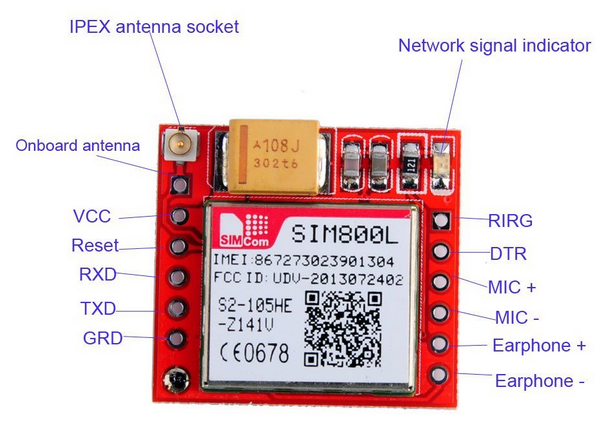
\includegraphics[width=0.7\textwidth]{sim800l}
\caption[Sơ đồ module sim800l]{Sơ đồ module sim800l}
\label{fig:sim800l}
\end{figure}

\begin{itemize}
\item[•]TXD: chân truyền UART TX
\item[•]RXD: chân nhận UART RX
\item[•]DTR: chân UART DTR, thường ít sử dụng.
\item[•]SPKP, SPKN: ngõ ra âm thanh, nối với loa để phát âm thanh.
\item[•]MICP, MICN: ngõ vào âm thanh, phải găn thêm micro để thu âm thanh.
\item[•]Reset: chân khởi động lại SIM800L
\item[•]RING: báo cuộc gọi đến
\item[•]GND: chân Mass, cấp 0v.
\end{itemize}

%/////////////////////////////////////////////////////////////////////////AT SIM 800L
\newpage
\subsubsection*{Một số tập lệnh AT của module Sim800L dùng trong đề tài luận văn}


 AT+CBC: trả về kết quả dung lượng pin hiện tại.
\begin{table}[H]
\label{table:at+cbc}
\begin{tabular}{|l|l|}
\hline
Lệnh AT & AT+CBC \\ \hline
Kết quả  & 
+ CBC: <bcs>, <bcl>, <voltage> \\
&OK \\
& \\
& Với các thông số \\
& \hspace{0.5cm} <bcs>: \\
& \hspace{2cm} • 0: Mạch không phải trạng thái đang sạc. \\
& \hspace{2cm} • 1: Mạch đang trong trạng thái sạc. \\
& \hspace{2cm} • 2: Mạch đã sạc xong. \\
& \hspace{0.5cm} <bcl>: giá trị \% dung lượng pin: 1 …100 \%. \\
& \hspace{0.5cm} <voltage>: Giá trị nguồn đầu vào của module sim (mV) \\\hline
\end{tabular}
\caption[Tập lệnh AT+CBC: kết quả dung lượng pin hiện tại]{Tập lệnh AT+CBC}
\end{table}



 AT+ CCLK trả về giá trị thời gian của module sim
\begin{table}[H]
\label{table:at+cclk}
\begin{tabular}{|l|l|}
\hline
Lệnh AT & AT+CCLK \\ \hline
Kết quả  & 
+ CBC: <time> \\
&OK \\
& \\
& Với các thông số \\
& \hspace{0.5cm}<time>: là một dạng chuỗi String, chuỗi String này được format\\
& \hspace{0.5cm} dưới dạng $yy/MM/dd, hh:mm:ss+-zz$ \\\hline
\end{tabular}

\caption[Tập lệnh AT+CCLK: trả về giá trị thời gian của module sim]{Tập lệnh AT+CCLK}
\end{table}

\newpage

AT+CSTT cài đặt các thông số APN, USER NAME, PASSWORD cho Sim
\begin{table}[H]
\label{table:at+cstt}
\begin{tabular}{|l|l|}
\hline
Lệnh AT & AT+CSTT= <apn>,<user>,<password> \\ 
& \\
& \hspace{0.5cm}<apn> Địa điểm truy cập GPRS\\
& \hspace{0.5cm}<user> Tên đăng nhập\\
& \hspace{0.5cm}<pass> Mật khẩu đăng nhập\\
& \\
& 3 thông số trên được cung cấp theo từng nhà mạng của mỗi sim khi \\
& được gắn vào module sim, mục đích dùng để xác nhận việc truy cập \\
& GPRS vào các nhà mạng.\\
& Ví dụ thông số của nhà mạng vinaphone: <m3-world>,<mms>,<mms> \\\hline
Kết quả  &+ OK \\\hline
\end{tabular}

\caption[Tập lệnh AT+CSTT: cài đặt các thông số APN, USER NAME, PASSWORD cho Sim]{Tập lệnh AT+CSTT}
\end{table}





AT+CIFSR: Lấy thông tin địa chỉ IP của moduleSIM
\begin{table}[H]
\label{table:AT+CIFS}
\begin{tabular}{|l|l|}
\hline
Lệnh AT & AT+CIFSR \\ \hline
Kết quả  & 
<IP address> \\
& \\
& <IP address>: địa chỉ IP được gắn sau khi tham gia vào GPRS.\\\hline
\end{tabular}

\caption[Tập lệnh AT+CIFSR: lấy thông tin địa chỉ IP của moduleSIM]{Tập lệnh AT+CIFSR}
\end{table}

\newpage


AT+CIPSTART: thiết lập kết nối TCP hoặc UDP
\begin{table}[H]
\label{table:AT+CIPSTART}
\begin{tabular}{|l|l|}
\hline
Lệnh AT & AT+CIPSTART=”TCP”,”192.168.0.1”,”80” \\ 
& Kết nối tới địa chỉ 192.168.0.1 tại cổng 80 với giao thức TCP.\\
& \\
& AT+CIPSTART=”UDP”,”192.168.0.1”,”8888” \\ 
& Kết nối tới địa chỉ 192.168.0.1 tại cổng 8888 với giao thức UDP.\\ \hline
Kết quả  &+ OK \\
& \\
& CONNECT OK\\\hline
\end{tabular}

\caption[Tập lệnh AT+CIPSTART: thiết lập kết nối TCP hoặc UDP]{Tập lệnh AT+CIPSTART}
\end{table}


AT+CDNSGIP: được dùng để phân giải DNS của một tên miền, nó được sử dụng cho việc thiếp lập kết nối TCP/UCP thông qua tên miền bằng câu lệnh “AT+CIPSTART=<mode>,<domain name>, <port>”, và sau đó người dùng có thể gửi dữ liệu đến máy chủ thông qua câu lệnh AT+CIPSEND.
\begin{table}[H]
\label{table:AT+CDNSGIP}
\begin{tabular}{|l|l|}
\hline
Lệnh AT & AT+CDNSGIP=<domain name> \\ 
& \\
& <domain name>: Tên miền muốn phân giải DNS, \\

& ví dụ như AT+CDNSGIP= “www.codingyourfuture.com “\\ \hline
Kết quả  &OK \\
&+ CDNSGIP:\\
&1,”www.codingyourfuture.com”,”113.173.153.194”,”119.75.217.56”\\\hline
\end{tabular}

\caption[Tập lệnh AT+CDNSGIP: phân giải DNS tên miền]{Tập lệnh AT+CDNSGIP}
\end{table}








\newpage



AT+CIPSEND: gửi dữ liệu thông qua giao thức kết nối TCP/UCP
\begin{table}[H]
\label{table:AT+CIPSEND}
\begin{tabular}{|l|l|}
\hline
Lệnh AT & AT+CIPSEND=<length> \\ 
& \\
& <length>: độ dài dữ liệu muốn gửi.\\\hline
Kết quả  & >  \\ \hline
Lệnh AT & Dữ liệu muốn gửi đi \\ \hline
Kết quả  & OK  \\ \hline
\end{tabular}

\caption[Tập lệnh AT+CIPSEND: gửi dữ liệu qua giao thức TCP/UCP]{Tập lệnh AT+CIPSEND}
\end{table}



\subsection{Pin năng lượng mặt trời}
Pin năng lượng mặt trời (pin mặt trời/pin quang điện) là thiết bị giúp chuyển hóa trực tiếp năng lượng ánh sáng mặt trời (quang năng) thành năng lượng điện (điện năng) dựa trên hiệu ứng quang điện. Hiệu ứng quang điện là khả năng phát ra điện tử (electron) khi được ánh sáng chiếu vào của vật chất.

Tấm pin mặt trời, những tấm có bề mặt lớn thu thập ánh nắng mặt trời và biến nó thành điện năng, được làm bằng nhiều tế bào quang điện có nhiệm vụ thực hiện quá trình tạo ra điện từ ánh sáng mặt trời.
\begin{figure}[H]
\centering    
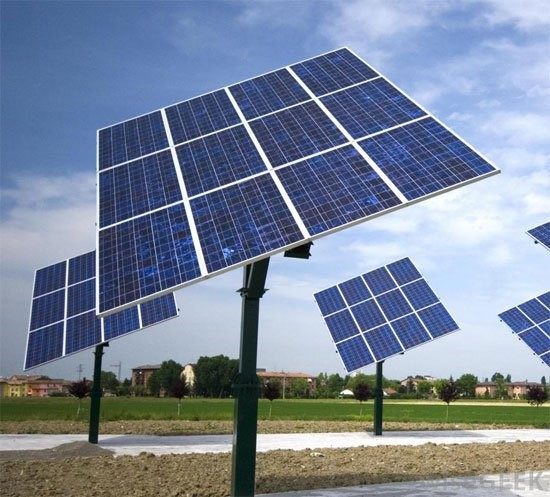
\includegraphics[width=0.7\textwidth]{solarpanel}
\caption[Tấm pin năng lượng mặt trời]{Tấm pin năng lượng mặt trời}
\label{fig:solarpanel}
\end{figure}

\subsubsection*{Chất bán dẫn Silicon}
Silicon được biết đến là một chất bán dẫn. "Chất bán dẫn là vật liệu trung gian giữa chất dẫn điện và chất cách điện. Chất bán dẫn hoạt động như một chất cách điện ở nhiệt độ thấp và có tính dẫn điện ở nhiệt độ phòng". Với tính chất như vậy, silicon là một thành phần quan trọng trong cấu tạo của pin năng lượng mặt trời.

Silicon tuy có mức dẫn điện hạn chế nhưng nó có cấu trúc tinh thể rất phù hợp cho việc tạo ra chất bán dẫn. Nguyên tử silicon cần 4 electron để trung hòa điện tích nhưng lớp vỏ bên ngoài một nguyên tử silicon chỉ có một nửa số electron cần thiết nên nó sẽ bám chặt với các nguyên tử khác để tìm cách trung hòa điện tích.

Để tăng độ dẫn điện của silicon, các nhà khoa học đã “tạp chất hóa” nó bằng cách kết hợp nó với các vật liệu khác. Quá trình này được gọi là “doping” và silicon pha tạp với các tạp chất tạo ra nhiều electron tự do và lỗ trống. Một chất bán dẫn silicon có hai phần, mỗi phần được pha tạp với một loại vật liệu khác. Phần đầu tiên được pha với phốt pho, phốt pho cần 5 electron để trung hòa điện tích và có đủ 5 electron trong vỏ của nó. Khi kết hợp với silicon, một electron sẽ bị dư ra. Electron đặc trưng cho điện tích âm nên phần này sẽ được gọi là silicon loại N (điện cực N). Để tạo ra silicon loại P (điện cực P), các nhà khoa học kết hợp silicon với boron. Boron chỉ cần 3 electron để trung hòa điện tích và khi kết hợp với silicon sẽ tạo ra những lỗ trống cần được lấp đầy bởi electron.
\begin{figure}[H]
\centering    
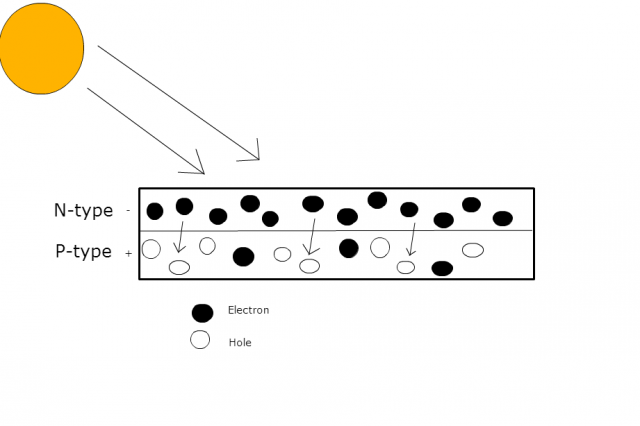
\includegraphics[width=0.7\textwidth]{solarpanel_hinhthanhdientich}
\caption[Tấm pin năng lượng mặt trời]{Tấm pin năng lượng mặt trời}
\label{fig:solarpanel_hinhthanhdientich}
\end{figure}


Khi chất bán dẫn silicon tiếp xúc với năng lượng, các electron tự do ở điện cực N sẽ di chuyển sang để lấp đầy các lỗ trống bên điện cực P. Sau đó, các electron từ điện cực N và điện cực P sẽ cùng nhau tạo ra điện trường. Các tế bào năng lượng mặt trời sẽ trở thành một diode, cho phép electron di chuyển từ điện cực P đến điện cực N, không cho phép di chuyển ngược lại.

Tất nhiên, để kích hoạt quá trình cần có năng lượng tiếp xúc với các tế bào silicon. Ánh sáng mặt trời bao gồm các hạt rất nhỏ gọi là photon được tỏa ra từ mặt trời, các hạt nhỏ năng lượng có thể tiếp xúc với các tế bào năng lượng mặt trờivà nới lỏng liên kết của các electron ở điện cực N. Sự di chuyển của các elentron tự do từ điện cực N tới điện cực P tạo ra dòng điện.





\subsubsection*{Hiệu suất của pin mặt trời}
Các công nghệ biến ánh sáng mặt trời thành điện hiện tại vẫn kém hiệu quả. Các tấm pin mặt trời chưa thể hấp thụ toàn bộ năng lượng của ánh sáng mặt trời. Nói chung, những tế bào năng lượng mặt trời tốt nhất hiện tại chỉ có thể chuyển 25\% năng lượng mà nó nhận được thành điện. Tại sao vậy? Thực tế là ánh sáng mặt trời, như tất cả các loại ánh sáng khác, bao gồm một quang phổ với các bước sóng khác nhau, mỗi bước sóng có một cường độ khác nhau. Có những bước sóng quá yếu không thể giải phóng các electron còn một số bước sóng lại quá mạnh với silicon.

\section{Công cụ hỗ trợ phát triển đề tài}
\subsection{Thingspeak}
ThingSpeak là một mã nguồn mở cho các ứng dụng của Internet of Things. Mã nguồn này hỗ trợ các API lưu trữ, lấy dữ liệu từ các thiết bị, sản phẩm sử dụng HTTP qua Internet hoặc thông qua một Local Area Network. Như một HUB đợi các thông tin cảm biến từ thiết bị và có nhiệm vụ lưu trữ và xử lý dữ liệu, với ThingSpeak, bạn có thể tạo ra các ứng dụng phân tích dữ liệu, lưu trữ dữ liệu, quản lý dữ liệu một cách đơn giản.\\
ThinkSpeak được phát triển bởi ioBridge và được opensource trên GITHUB  \url{https://github.com/iobridge/thingspeak}

\begin{figure}[H] 
\centering    
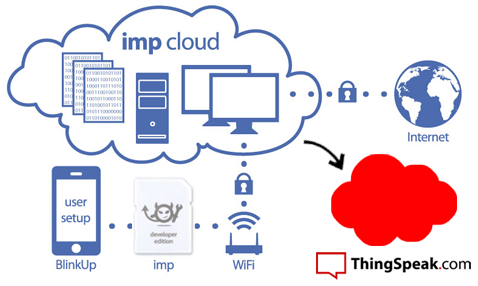
\includegraphics[width=0.7\textwidth]{thingspeak}
\caption[Ứng dụng phát triển IoT Thingspeak]{Ứng dụng phát triển IoT Thingspeak}
\label{fig:thingspeak}
\end{figure}

\section{Kiến thức căn bản công nghệ được áp dụng}

\subsection{Web API} 

Web API là giao diện lập trình ứng dụng (API – Application Programming Interface) cho cả web server và web browser.\cite{c2api}

Web API giúp người phát triển xây dựng lên các Service cung cấp dịch vụ cho các ứng dụng web, window… Trước web API, để có các service API người dùng phải cấu hình, xây dựng các ứng dụng wcf, web service khá phức tạp. Các ứng dụng client như website, ứng dụng winform, wpf có thể kết nối vào Web API để lấy các dữ liệu về xử lý, cũng như cập nhật thông tin lại Web API.

Web API dùng phương thức trao đổi dữ liệu là HTTP, kiểu dữ liệu trao đổi có thể là JSON, XML, hoặc một chuẩn dữ liệu bất kỳ. Đây là những chuẩn dữ liệu hướng đối tượng được dùng khá nhiều trong việc lưu chuyển thông tin trên Internet, do đó các trang web sử dụng web API tương tác dữ liệu có tốc độ khá cao. Ngoài ra do Web API dùng giao thức HTTP nên hầu như tất cả các ứng dụng trên các công nghệ đều có thể kết nối tới để lấy cũng như tương tác với web API cụ thể như chúng ta có thể dùng các công nghệ web như: Asp.NET (MVC, Web Page, WebForm), PHP, jsp hay các ứng dụng desktop như: winform, wpf đều có thể dễ dàng kết nối tới web API. Với Web API chúng ta có thể xây dựng và phân tách các ứng dụng web lớn, cấu hình từng thành phần riêng biệt của website: đâu là tầng data, đâu là tầng xử lý, đâu là tầng dịch vụ, … Nền tảng của các ứng dụng lớn luôn là các service để các website thành viên có thể kết nối tương tác dữ liệu. Do đó với Web API chúng ta có thể ứng dụng vào các dự án web (cũng như window) lớn để phát triển trên nhiều tầng xử lý khác nhau. Dùng Web API chúng ta dễ dàng xây dựng các ứng dụng window kiểu điện toán (dữ liệu ở server) còn client chỉ cài giao diện, hay có thể xây dựng các website Single Page Application (SPA – tất cả web chỉ gói gọn trong một trang). Ứng dụng này tương tác khá cao với người dùng, tốc độ nhanh (do dùng ajax, sẽ được nói rõ hơn ở phần sau) thường được dùng làm các website tương tác với các thiết bị di động (các thiết bị di động thường có kết nối Internet chậm).

\subsection{Căn bản về RESTful Web services}

\textbf{Tổng quan về REST – Representational State Transfer}

REST là một kiểu kiến trúc dựa trên các tiêu chuẩn web và giao thức HTTP. REST được mô tả đầu tiên bởi Roy Fielding trong luận văn tiến sĩ của ông vào năm 2000.

Trong một kiến trúc REST thì tất cả mọi thứ là một nguồn tài nguyên. Một nguồn tài nguyên được truy cập thông qua một giao diện phổ biển dựa trên các phương pháp tiêu chuẩn HTTP.

Một kiến trúc REST thường có một REST server cung cấp truy cập đến các nguồn tài nguyên và một Rest client truy cập và trình sửa các tài nguyên đó.

REST cho phép các nguồn tài nguyên biểu diễn dưới nhiều kiểu khác nhau như Text, XML, JSON … Rest client có thể yêu cầu một kiểu biểu diễn cụ thể thông qua giao thức HTTP.

\textbf{Các phương thức HTTP}

Các phương thức PUT, GET, POST và DELETE thường được sử dụng trong kiến trúc REST

• \textbf{GET} định nghĩa một truy cập đọc nguồn tài nguyên mà không có tác dụng phụ. Nguồn tài nguyên không bao giờ thay đổi thông qua một yêu cầu GET.

• \textbf{PUT} dùng để tạo một tài nguyên mới.

• \textbf{DELETE} loại bỏ các nguồn tài nguyên.

• \textbf{POST} cập nhật một nguồn tài nguyên hiện có hoặc tạo ra một nguồn tài nguyên mới.

\textbf{RESTful webservice}

Một RESTful webservice được dựa trên các phương thức HTTP và các khái niệm về REST. Một RESTful webservice thường xác định URI cơ sở cho các dịch vụ, hỗ trợ các kiểu MIME (XML, Text, JSON,…) và tập các hoạt động (POST, GET, PUT, DELETE) đều được hỗ trợ.

\textbf{JSON (JavaScript Object Notation)}

Là một định dạng hoán vị dữ liệu nhanh. Chúng dễ dàng cho chúng ta đọc và viết. Dễ dàng cho thiết bị phân tích và phát sinh. Chúng là cơ sở dựa trên tập hợp của Ngôn Ngữ Lập Trình JavaScript, tiêu chuẩn ECMA-262 phiên bản 3 – tháng 12 năm 1999. JSON là một định dạng kiểu text mà hoàn toàn độc lập với các ngôn ngữ hoàn chỉnh, thuộc họ hàng với các ngôn ngữ họ hàng C, gồm có C, C++, C, Java, JavaScript, Perl, Python, và nhiều ngôn ngữ khác. Những đặc tính đó đã tạo nên JSON một ngôn ngữ hoán vị dữ liệu lý tưởng.

JSON được xây dựng trên 2 cấu trúc:

• Là tập hợp của các cặp tên và giá trịname – value. Trong những ngôn ngữ khác nhau, đây được nhận thấy như là một đối tượng (object), sự ghi (record), cấu trúc (struct), từ điển (dictionary), bảng băm (hash table), danh sách khóa (keyed list), hay mảng liên hợp.

• Là một tập hợp các giá trị đã được sắp xếp. Trong hầu hết các ngôn ngữ, nó được nhận thấy như là một mảng, vector, list hay là một dãy sequence.


\begin{figure}[H]
	\centering    
	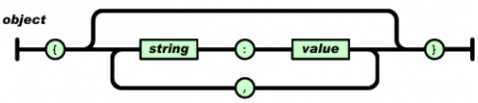
\includegraphics[width=1.0\textwidth]{json0}
	\caption[Cấu trúc của một đối tượng JSON]{Cấu trúc của một đối tượng JSON}
	\label{fig: json0}
\end{figure}

Một đối tượng là một tập hợp của các cặp tên/giá trị (name/value). Một đối tượng bắt đầu bởi dấu “{“ và kết thúc với dấu “}”. Từng tên được theo sau bởi dấu “:” và các cặp tên/giá trị được tách ra bởi dấu “,”.

\begin{figure}[H]
	\centering    
	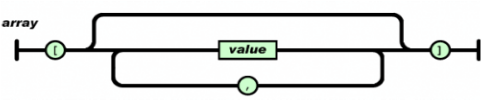
\includegraphics[width=1.0\textwidth]{json1}
	\caption[Cấu trúc mảng của JSON]{Cấu trúc mảng của JSON}
	\label{fig: json1}
\end{figure}

Một mảnglà một tập hợp các giá trị đã được xắp xếp, một mảng bắt đầu bởi dấu “[” và kết thúc với dấu “]”. Các giá trị được cách nhau bởi dấu “,”.
\begin{figure}[H]
	\centering    
	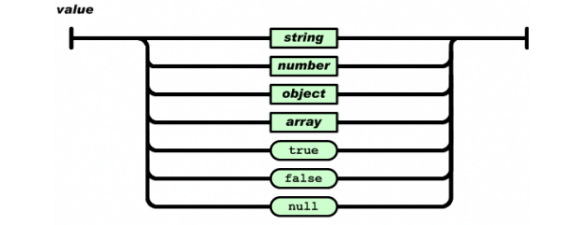
\includegraphics[width=1.0\textwidth]{json2}
	\caption[Cấu trúc của một đối tượng JSON]{Cấu trúc của một đối tượng JSON}
	\label{fig: json2}
\end{figure}

Một giá trị có thể là chuổi, số, đúng sai, hoặc là đối tượng hoặc mảng. Những cấu trúc này có thể được lồng vào nhau.

\textbf{JSON và Webservice}

Việc trao đổi thông tin, truyền tải dữ liệu giữa Webservice và ứng dụng người ta thường dùng XML hay JSON vì sự tiện nghi và cấu trúc dữ liệu nhỏ gọn của nó. JSON là một ngôn ngữ mới với tuổi đời con trẻ nhưng vẫn được ứng dụng nhiều bới những điểm lợi của nó:

• “Con người” có thể đọc được.

• Cú pháp gần với JavaScript nên rất dễ để sử dụng.

• Dữ liệu truyền tải ngắn gọn so với những định dạng dữ liệu như: XML, HTML…

• Việc phân tích (parse) dữ liệu từ dạng chuỗi (nhận từ server) sang dữ liệu có thể sử dụng được (thành Object, Number, Array) dễ dàng.
\begin{figure}[H]
	\centering    
	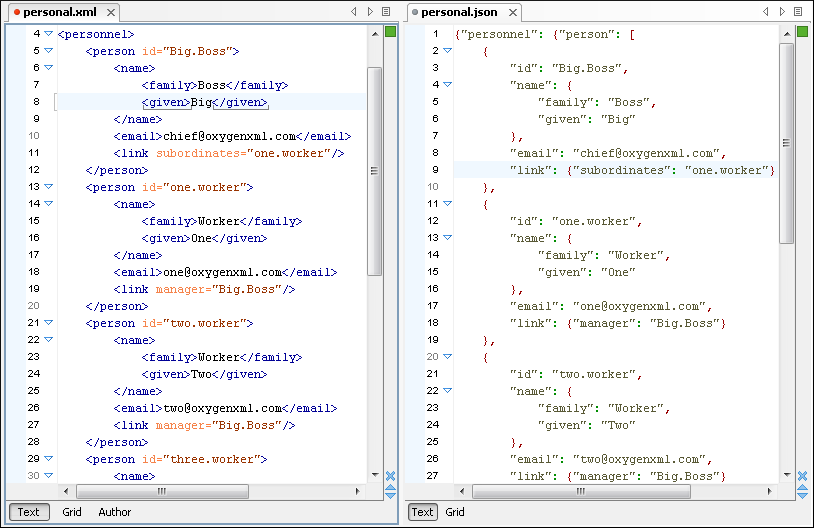
\includegraphics[width=1.0\textwidth]{json3}
	\caption[Cấu trúc mô tả XML-JSON]{Cấu trúc mô tả XML-JSON}
	\label{fig: json3}
\end{figure}
Nhằm mục đích giúp thời gian tương tác giữa người sử dụng với ứng dụng tiến gần đến thời gian thực, thì tốc độ được đặt lên hàng đầu, việc tăng tốc bằng cách “giảm tải” cũng là một giải pháp, chính vì vậy JSON được ưu ái hơn vì cú pháp ngắn gọn, đơn giản, tiết kiệm hơn XML.



\subsection{NodeJs}
NodeJS là một nền tảng Server side được xây dựng dựa trên Javascript Engine (V8 Engine). Node.js được phát triển bởi Ryan Dahl năm 2009. Định nghĩa Nodejs bởi tài liệu chính thức : Node.js là một nền tảng dựa vào Chrome Javascript runtime để xây dựng các ứng dụng nhanh, có độ lớn.  \cite{c2node}

\begin{figure}[H]
	\centering    
	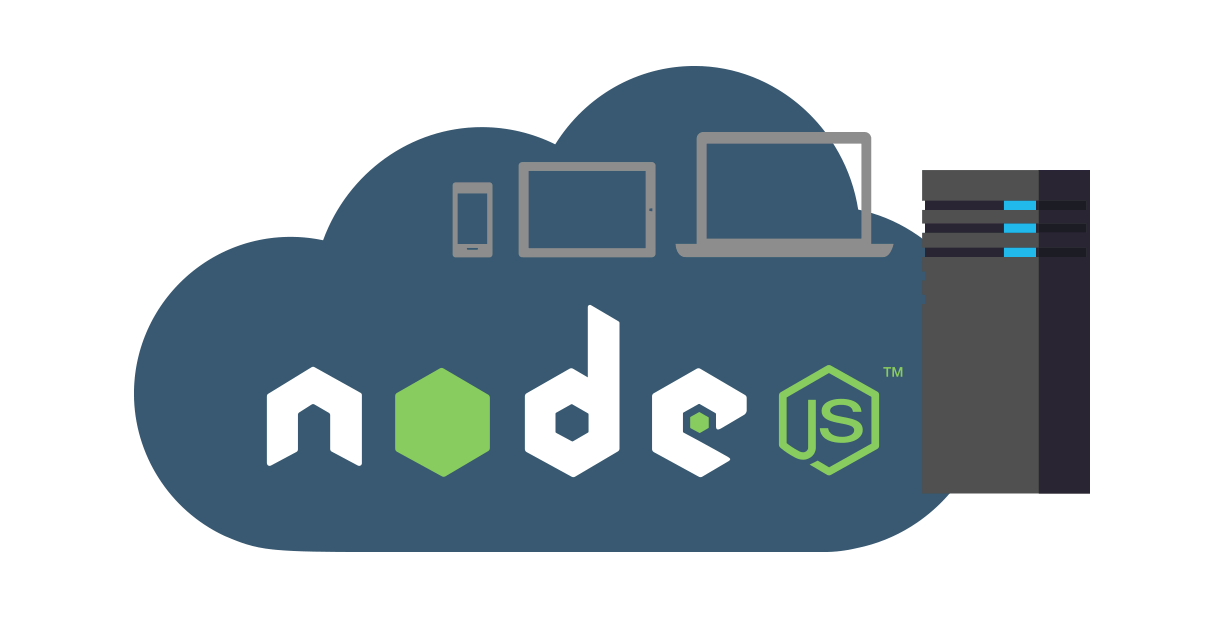
\includegraphics[width=1.0\textwidth]{nodejs0}
	\caption[Nền tảng Nodejs]{Nền tảng Nodejs}
	\label{fig: nodejs0}
\end{figure}

Node.js sử dụng các phần phát sinh các sự kiện (event-driven), mô hình non-blocking I/O để tạo ra các ứng dụng nhẹ và hiệu quả cho các ứng dụng về dữ liệu thời gian thực chạy trên các thiết bị phân tán.

\begin{figure}[H]
	\centering    
	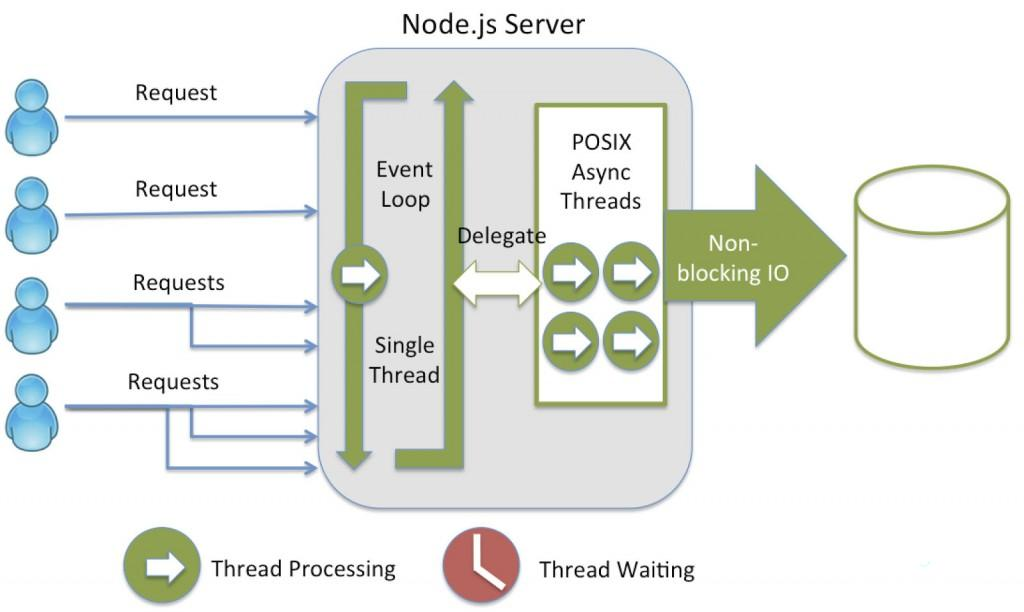
\includegraphics[width=1.0\textwidth]{nodejs1}
	\caption[Mô hình hoạt động Nodejs]{Mô hình hoạt động Nodejs}
	\label{fig: nodejs1}
\end{figure}

\subsection{Javascripts}
JavaScript, theo phiên bản hiện hành, là một ngôn ngữ lập trình kịch bản dựa trên đối tượng được phát triển từ các ý niệm nguyên mẫu. Ngôn ngữ này được dùng rộng rãi cho các trang web, nhưng cũng được dùng để tạo khả năng viết script sử dụng các đối tượng nằm sẵn trong các ứng dụng. Nó vốn được phát triển bởi Brendan Eich tại Hãng truyền thông Netscape với cái tên đầu tiên Mocha, rồi sau đó đổi tên thành LiveScript, và cuối cùng thành JavaScript. Giống Java, JavaScript có cú pháp tương tự C, nhưng nó gần với Self hơn Java. .js là phần mở rộng thường được dùng cho tập tin mã nguồn JavaScript.\cite{c2js}

Những ứng dụng to lớn của Javascript khiến người ta không thể quên nó được. Hiện nay có rất nhiều libraries, Framework được viêt như: \cite{c2js2}

• AngularJS: Một thư viện dùng để xây dựng ứng dụng Single Page

• NodeJS: Một thư viện được phát triển phía Server dùng để xây dựng ứng dụng realtime

• Sencha Touch: Một Framework  dùng để xây dựng ứng dụng Mobile

• ExtJS: Một Framework dùng xây dựng ứng dụng quản lý (Web Applications)

• jQuery: Một thư viện rất mạnh về hiểu ứng

\subsection{Websocket - Socket.io}
WebSoket là công nghệ hỗ trợ giao tiếp hai chiều giữa client và server bằng cách sử dụng một TCP socket để tạo một kết nối hiệu quả và ít tốn kém. Mặc dù được thiết kế để chuyên sử dụng cho các ứng dụng web, lập trình viên vẫn có thể đưa chúng vào bất kì loại ứng dụng nào.\cite{c2wk}
\begin{figure}[H]
	\centering    
	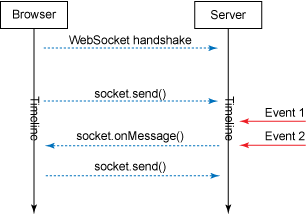
\includegraphics[width=0.7\textwidth]{websk}
	\caption[Mô hình hoạt động Websocket]{Mô hình hoạt động Websocket\cite{c2wk2}} 
	\label{fig: websk}
\end{figure}

Kết nối được duy trì có thể viết và nhận dữ liệu bằng JavaScript như khi bạn đang sử dụng một TCP socket đơn thuần.

So sánh dung lượng giữa hai hình thức sử dụng polling HTTP và Websocket trong việc truyền 10000 gói tin:

- HTTP: 871 x 10,000 = 8,710,000 bytes

- WebSocket: 2 x 10,000 = 20,000 bytes



\subsection{Socket.IO}

Socket.IO là một thư viện javascript có mục đích tạo ra các ứng dụng realtime trên trình duyệt cũng như thiết bị di động. Việc sử dụng thư viện này cũng rất đơn giản và giống nhau ở cả server lẫn client. 
\begin{figure}[H]
	\centering    
	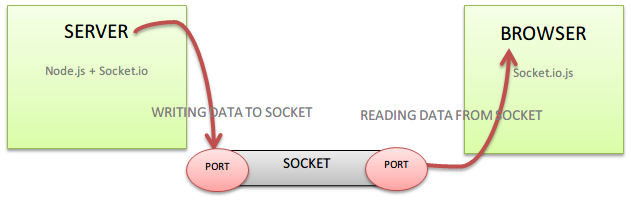
\includegraphics[width=0.9\textwidth]{socketio}
	\caption[Mô hình cơ bản của Socket.IO]{Mô hình cơ bản của Socket.IO}
	\label{fig: socketio}
\end{figure}
\textbf{Tại sao Socket.IO ra đời?}

\begin{itemize}
\item[•]Javascript là ngôn ngữ lập trình hướng sự kiện, mà trong lập trình thời gian thực, cách tiếp cận bằng lập trình sự kiện là cách tiếp cận khôn ngoan nhất.
\item[•]Node.js chạy non-blocking việc hệ thống không phải tạm ngừng để xử lý xong một request sẽ giúp cho server trả lời client gần như ngay tức thì.
\item[•]Lập trình socket yêu cầu bạn phải xây dựng được mô hình lắng nghe – trả lời từ cả 2 bên. Nói khác đi, vai trò của client và server phải tương đương nhau, mà client thì chạy bằng javascript, nên nếu server cũng chạy bằng javascript nữa, thì việc lập trình sẽ dễ dàng và thân thiện hơn.
\end{itemize}
Bởi vì thế, socket.io được ra đời để để phát triển việc giao tiếp theo thời gian thực giữa client và server dựa trên sức mạnh có sẵn của Javascript và Nodejs.
\begin{figure}[H]
	\centering    
	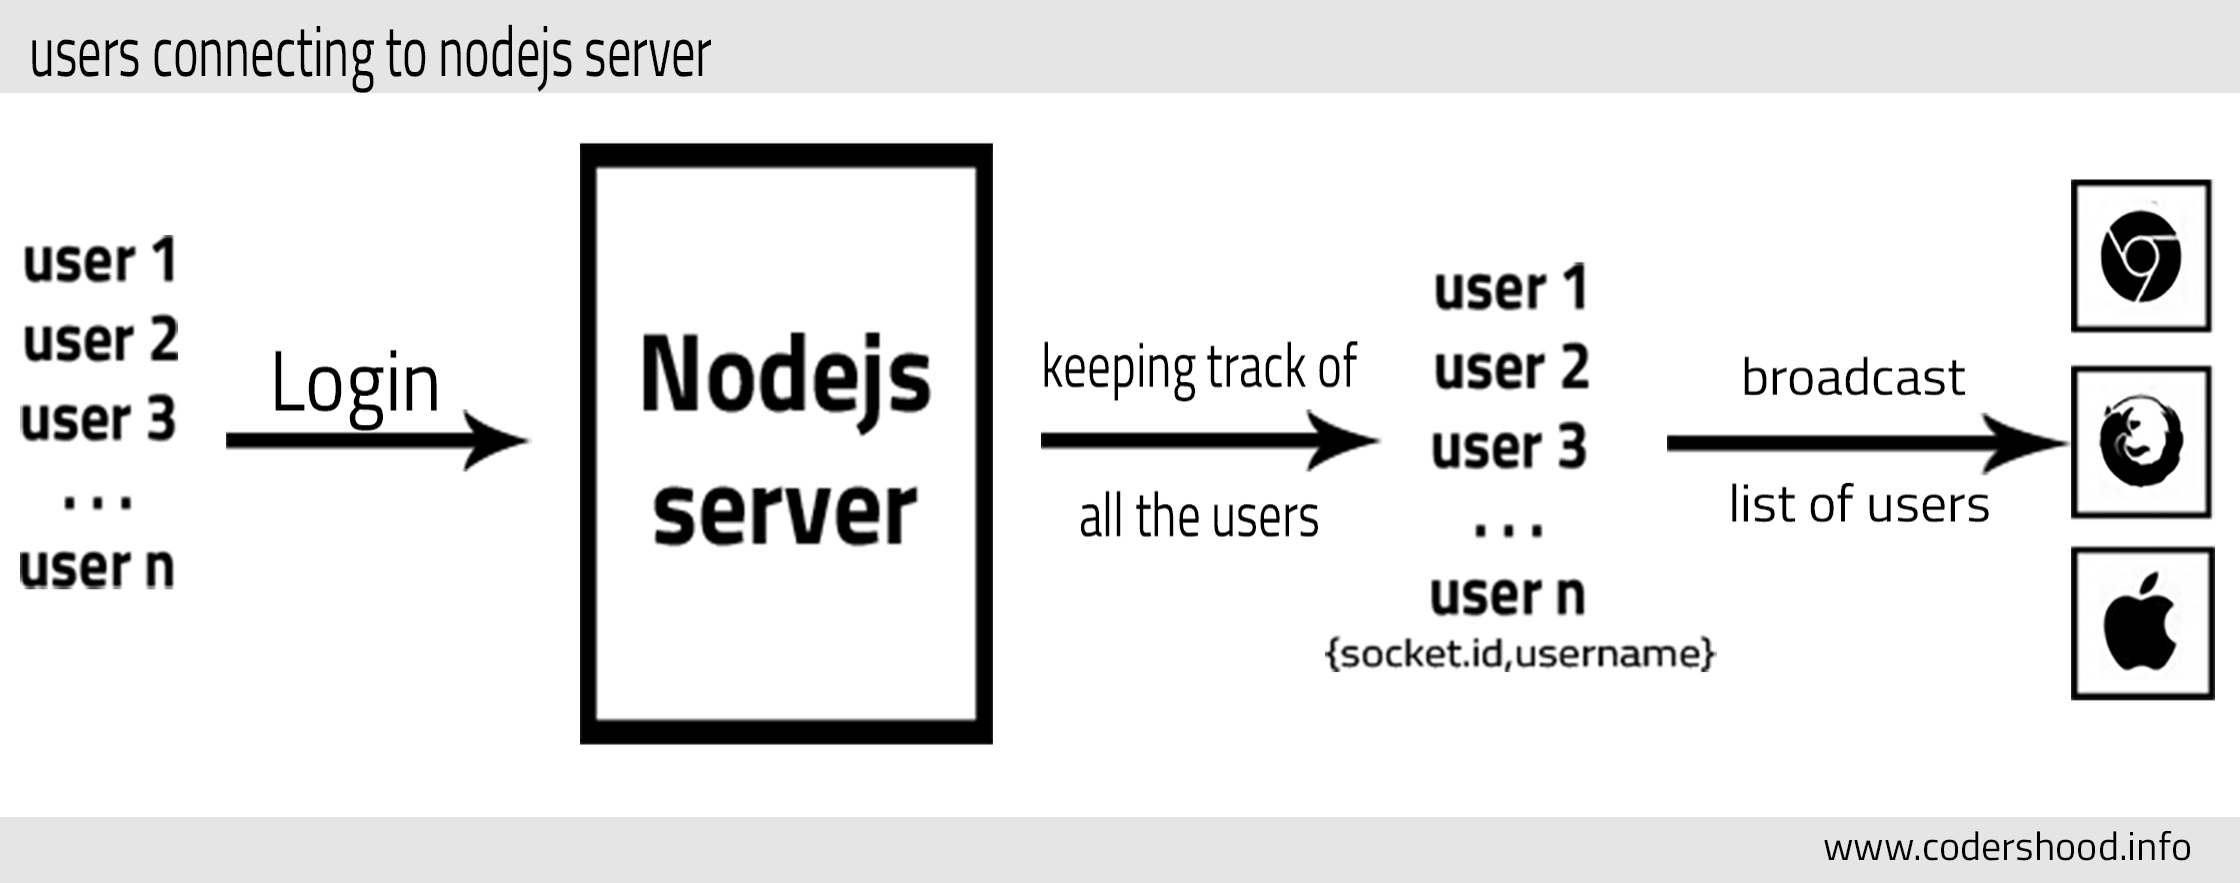
\includegraphics[width=0.9\textwidth]{socketio2}
	\caption[Mô hình hoạt động giao tiếp của Socket.IO]{Mô hình hoạt động giao tiếp của Socket.IO}
	\label{fig: socketio2}
\end{figure}
Socket.IO hoạt động dựa trên các events tương tự như Websocket:

• \textbf{connect()}: kết nối với server socket

• \textbf{on(event\_name, listener)}: đăng kí lắng nghe sự kiện từ server trả về

• \textbf{emit(event\_name, data)}: gửi một sự kiện lên server

• \textbf{off(event\_name)}: ngừng lắng nghe một sự kiện nào đó

\subsection{RethinkDB}

\textbf{RethinkDB là gì?}

RethinkDB là một mã nguồn mở, dựa theo cấu trúc cơ sở dữ liệu NoSQL \cite{c2nosql}, tổ chức dữ liệu theo kiểu document-oriented database - một thiết kế riêng biệt cho việc lưu trữ document. Các cài đặt có thể là giả lập tương tác trên relational database, object database hay key-value store. Cơ sở dữ liệu được lưu trữ dưới dạng JSON  với các giản đồ động, và được thiết kế giúp hoạt động dễ dàng trong việc cập nhật và truy xuất dữ liệu theo thời gian thực với các ứng dụng. \cite{c2rethink}

\begin{figure}[H]
	\centering    
	
\includegraphics[width=1\textwidth]{rethinkdb}
	\caption[Biểu tượng của RethinkDB]{Biểu tượng của RethinkDB}
	\label{fig: rethinkdb}
\end{figure}

RethinkDB sử dụng ngôn ngữ truy vấn ReQL được phát triển theo hướng đối tượng. Và ngôn ngữ này hỗ trợ cho các thao tác nhập bảng, quản lý nhóm, tích hợp và các hàm chức năng truy vấn cũng như event theo thời gian thực.

\begin{figure}[H]
	\centering    
	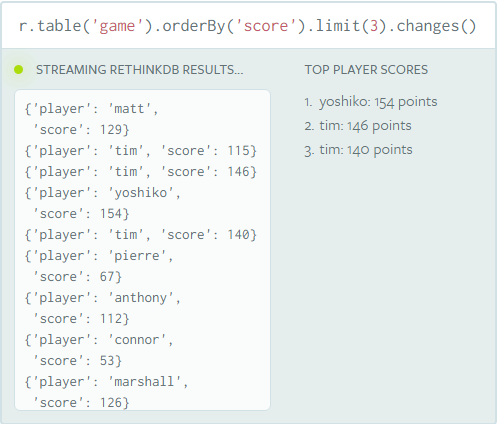
\includegraphics[width=0.9\textwidth]{rethink1}
	\caption[Đoạn code mẫu RethinkDB]{Đoạn code mẫu RethinkDB}
	\label{fig: rethink1}
\end{figure}

Như hình \ref{fig: rethink1} là ví dụ trực quan được demo trực tiếp tại trang chủ https://www.rethinkdb.com, có thể nhận thấy được cách thức khai báo và sử dụng RethinkDB:

• \textbf{r} : là đối tượng RethinkDB chúng ta khai báo trong ứng dụng.

• \textbf{table()} : là bảng giá trị đang truy vấn.

• \textbf{orderBy()} : hàm sắp xếp dữ liệu theo trường giá trị được khai báo.

• \textbf{limit()} : chọn ra những giá trị trong phạm vi được khai báo trong hàm.

• \textbf{changes()} : đây chính là đặc điểm khiến RethinkDB khác biệt so với các hệ quản lý dữ liệu khác. RethinkDB sẽ gọi hàm thực thi khi vùng giá trị truy vấn có thay dổi giá trị theo thời gian thật. không hoạt động theo cơ chế polling thường thấy ở các kiểu truy vấn dữ liệu khác.

\subsection{Raspberry}

Raspbian là hệ điều hành mở và miễn phí được phát triển tối ưu hóa dựa trên nền Debian dành riêng cho thiết bị phần cứng Raspberry Pi. Hệ điều hành này bao gồm nhóm các chức năng và ứng dụng giúp Raspberry hoạt động. Hơn nữa, Raspbian cung cấp nhiều hơn là hệ điều hành thuần: hỗ trợ tới hơn 35,000 gói mở rộng và dễ dàng cài đặt trên Raspberry Pi. Raspbian ổn định và hiệu suất cao được hoàn thiện vào tháng 6 năm 2012. Tuy nhiên Raspbian vẫn đang được phát triển tới ngày nay và ngày càng cải thiện hiệu suất cũng như hỗ trợ các gói chức năng nhiều nhất có thể. \cite{c2rasp}
\begin{figure}[H]
	\centering    
	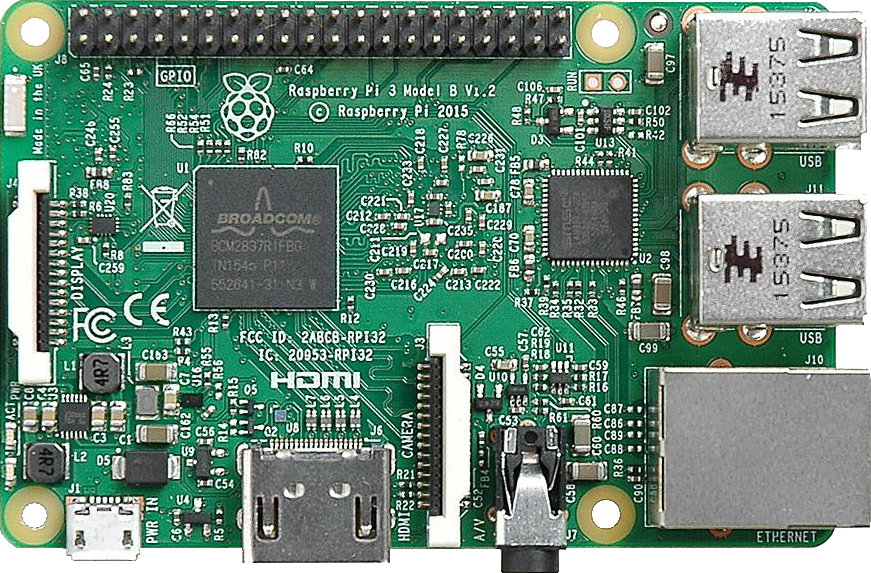
\includegraphics[width=0.9\textwidth]{rasp}
	\caption[Thiết bị Raspberry Pi]{Thiết bị Raspberry Pi}
	\label{fig: rasp}
\end{figure}

Vì sao lựa chọn Raspberry:

• Là một máy tính độc lập chạy trên nền tảng Linux, điều này làm cho việc chạy các ứng dụng Nodejs hay RethinkDB hoạt động được trên Raspberry Pi.

• Hiệu suất đáp ứng nhu cầu làm server của đề tài yêu cầu với mức độ tiêu thụ năng lượng cực kì ít.









\subsection{Framework Ionic}
\subsubsection*{Giới thiệu về Ionic framework}
Ionic là một framework được sử dụng để phát triển các ứng dụng di động dựa trên nền tảng công nghệ web HTML5 để tạo ra các ứng dụng lai hóa [ hybrid apps ] chạy trên các thiết bị di động khác nhau. Ứng dụng lai hóa ở đây được hiểu cơ bản là các ứng dụng chạy trên nền các trình duyệt được nhúng vào trong một ứng dụng được cài đặt và có thể giao tiếp, truy cập, điều khiển sử dụng các thiết bị phần cứng và hệ điều hành mobile.

Hãy tưởng tượng Ionic như là một khung phát triển giao diện người dùng để xử lý tất cả các tương tác giao diện người dùng làm cho ứng dụng trở nên thuyết phục và dễ dàng sử dụng. Kiểu như “Bootstrap for Native”, tức là như các ứng dụng Native nhưng có sự hỗ bởi một loạt các thành phần giao diện, động và thiết kế đẹp.

\begin{figure}[H]
\centering    
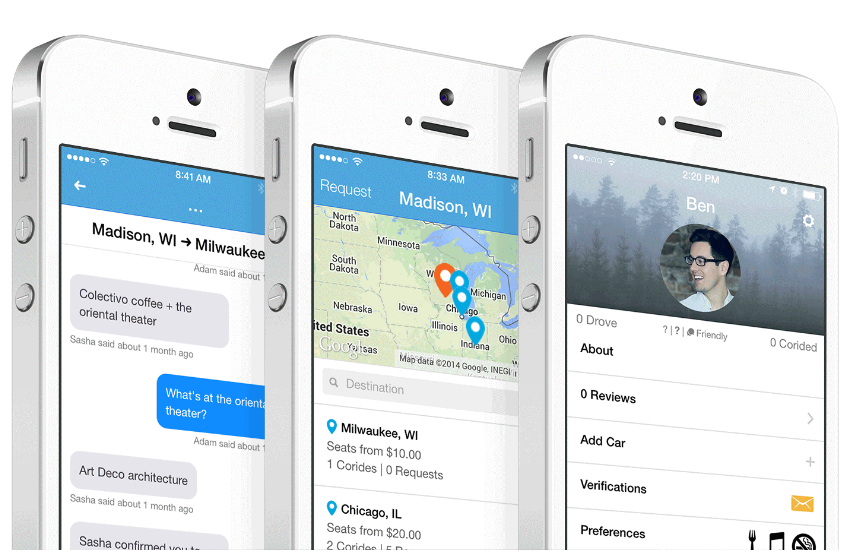
\includegraphics[width=0.7\textwidth]{ionic}
\caption[Một số giao diện của Ionic ]{Một số giao diện của Ionic}
\label{fig:ionic}
\end{figure}


Bản chất Ionic là một khung phát triển HTML5, nó cần một vỏ bọc native như Cordova hay PhoneGap để có thể khởi động như một ứng dụng native. Ionic được hỗ trợ mạnh mẽ bởi Cordova. Việc cài đặt và khởi tạo một dự án Ionic rất dễ dàng thông qua giao diện dòng lệnh dựa trên Node.js


\subsubsection*{Ưu điểm và nhược điểm của Ionic}

Ưu điểm:
\begin{itemize}
\item[•] Dễ học, thời gian phát triển nhanh, có thể sử dụng các kỹ năng từ lập trình web.
\item[•] Đa nền tảng.
\item[•] Khả năng truy cập đến các tính năng của thiết bị và hệ điều hành như bluetooth, camera,..
\item[•] Dễ dàng thiết kế giao diện cho các thiết bị có kích cỡ khác nhau
\item[•] Việc sử dụng AngularJS làm core giúp phần xử lý UI linh động hơn so với javasript hay thư viện Jquery.
\item[•] Việc sử dụng AngularJS làm core cũng mang lại lợi thế lớn so với các framework cho ứng dụng hybrid khác.
\item[•] Ionic cung cấp đầy đủ các thành phần trong giao diện người dùng như Pull-to-Refresh, Infinite-loader, tabs, …

\end{itemize}


Nhược điểm:


\begin{itemize}
\item[•] Vẫn còn trong giai đoạn phát triển.
\item[•] Hiệu năng vẫn chưa cao và ổn định.
\item[•] Cộng đồng phát triển ứng dụng vẫn còn chưa đông.
\end{itemize}

\subsection{Framework AngularJS}



Angular là một bộ Javascript Framework rất mạnh và thường được sử dụng để xây dựng project Single Page Application (SPA). Nó hoạt động dựa trên các thuộc tính mở rộng HTML (các atributes theo quy tắc của Angular). Đây là một Framework mã nguồn mở hoàn toàn miễn phí và được hàng ngàn các lập trình viên trên thế giới ưa chuộng và sử dụng.

\begin{figure}[H]
\centering    

\includegraphics[width=0.7\textwidth]{angularjs}
\caption[Angular JS kết hợp với ionic ]{Angular JS kết hợp với ionic}
\label{fig:angularjs}
\end{figure}

Ionic sử dụng AngularJS để cung cấp các cấu trúc ứng dụng, trong khi bản thân Ionic tập trung chính vào giao diện người dùng. Nói cách khác, chúng ta thấy được sự phối hợp ăn ý giữa sức mạnh của AngularJS và vẻ đẹp của Ionic UI.

Ionic cung cấp một tập các Angular directives (nghĩa là các phần tử HTML tùy biến) để làm các thành phần của nó, tạo ra sự dễ dàng để sử dụng các tiện ích gọn để viết mã HTML. Ngoài các directives, Ionic còn sử dụng và thêm vào các thành phần khác như: Angular touch recognizers, view animation logic, HTML sanitation, và asynchronous communication.

Việc xây dựng ứng dụng dựa trên AngularJS đòi hỏi mã nguồn phải có khả năng mở rộng cao để bổ sung các tính năng mới. Tuy nhiên với Ionic, người ta có thể tái sử dụng các chức năng trong ứng dụng trên các nền tảng khác nhau đồng thời vẫn có thể tùy chỉnh giao diện người dùng cho mỗi nền tảng riêng biệt. Các thành phần trong Ionic như danh sách, slide,.. chính là các directive(các thuộc tính của thẻ HTML dùng trong Angular) của AngularJS. Đó là lí do khiến cho Ionic và AngularJS kết hợp rất tốt với nhau.

Mặc dù, Ionic có thành phần giao diện sử dụng Angular, nhưng developers vẫn có thể sử dụng và hỗ trợ các framework khác như Knockout hay EmberJS.



\subsection{Framework Cordova}

\begin{figure}[H]
\centering    

\includegraphics[width=0.7\textwidth]{cordova}
\caption[Apache Cordova ]{Apache Cordova}
\label{fig:cordova}
\end{figure}

Apache Cordova là một bộ khung để xây dựng ứng dụng di động sử dụng HTML, CSS và Javascript. Apache Cordova bao gồm một tập hợp các API thiết bị cho phép người lập trình di động truy cập, sử dụng các chức năng native của thiết bị như là camera hay cảm biến gia tốc bằng Javascript. Kết hợp với một bộ khung phát triển giao diện như jQuery Mobile or Dojo Mobile hoặc Ionic, cho phép ứng dụng di động có thể được phát triển chỉ dựa trên HTML, CSS và Javascript.

Khi sử dụng Cordova API, một ứng dụng có thể được xây dựng mà không phải sử dụng bất kỳ một đoạn mã native code nào. Thay vào đó, công nghệ web sẽ được sử dụng, và chúng sẽ được tổ chức trên chính ứng dụng đấy chứ không cần thông qua một server nào.

Cordova cung cấp một tập hợp các thư viện Javascript đã được chuẩn hóa để có thể sử dụng. Cordova hiện có thể sử dụng cho các nền tảng như iOS, Android, Blackberry, Windows Phone, Palm WebOS, Bada và Symbian.


\chapter{Thiết kế và Hiện thực}



\section{Thiết kế hệ thống}
\subsection{Kiến trúc mô hình hệ thống}
\subsection{Các ràng buộc của hệ thống}
\subsection{Mô hình ứng dụng trình bày dữ liệu}




\section{Hiện thực}
\subsection{Các node cảm biến thu thập dữ liệu}
\subsection{Hệ thống Server lưu trữ dữ liệu và cung cấp API}
\subsection{Ứng dụng theo dõi dữ liệu và đánh giá}





% **************************** Define Graphics Path **************************
\ifpdf
    \graphicspath{{Chapter3/Figs/Raster/}{Chapter3/Figs/PDF/}{Chapter3/Figs/}}
\else
    \graphicspath{{Chapter3/Figs/Vector/}{Chapter3/Figs/}}
\fi

\section{First section of the third chapter}
And now I begin my third chapter here \dots

And now to cite some more people~\citet{Rea85,Ancey1996}

\subsection{First subsection in the first section}
\dots and some more 

\subsection{Second subsection in the first section}
\dots and some more \dots

\subsubsection{First subsub section in the second subsection}
\dots and some more in the first subsub section otherwise it all looks the same
doesn't it? well we can add some text to it \dots

\subsection{Third subsection in the first section}
\dots and some more \dots

\subsubsection{First subsub section in the third subsection}
\dots and some more in the first subsub section otherwise it all looks the same
doesn't it? well we can add some text to it and some more and some more and
some more and some more and some more and some more and some more \dots

\subsubsection{Second subsub section in the third subsection}
\dots and some more in the first subsub section otherwise it all looks the same
doesn't it? well we can add some text to it \dots

\section{Second section of the third chapter}
and here I write more \dots

\section{The layout of formal tables}
This section has been modified from ``Publication quality tables in \LaTeX*''
 by Simon Fear.

The layout of a table has been established over centuries of experience and 
should only be altered in extraordinary circumstances. 

When formatting a table, remember two simple guidelines at all times:

\begin{enumerate}
  \item Never, ever use vertical rules (lines).
  \item Never use double rules.
\end{enumerate}

These guidelines may seem extreme but I have
never found a good argument in favour of breaking them. For
example, if you feel that the information in the left half of
a table is so different from that on the right that it needs
to be separated by a vertical line, then you should use two
tables instead. Not everyone follows the second guideline:

There are three further guidelines worth mentioning here as they
are generally not known outside the circle of professional
typesetters and subeditors:

\begin{enumerate}\setcounter{enumi}{2}
  \item Put the units in the column heading (not in the body of
          the table).
  \item Always precede a decimal point by a digit; thus 0.1
      {\em not} just .1.
  \item Do not use `ditto' signs or any other such convention to
      repeat a previous value. In many circumstances a blank
      will serve just as well. If it won't, then repeat the value.
\end{enumerate}

A frequently seen mistake is to use `\textbackslash begin\{center\}' \dots `\textbackslash end\{center\}' inside a figure or table environment. This center environment can cause additional vertical space. If you want to avoid that just use `\textbackslash centering'


\begin{table}
\caption{A badly formatted table}
\centering
\label{table:bad_table}
\begin{tabular}{|l|c|c|c|c|}
\hline 
& \multicolumn{2}{c}{Species I} & \multicolumn{2}{c|}{Species II} \\ 
\hline
Dental measurement  & mean & SD  & mean & SD  \\ \hline 
\hline
I1MD & 6.23 & 0.91 & 5.2  & 0.7  \\
\hline 
I1LL & 7.48 & 0.56 & 8.7  & 0.71 \\
\hline 
I2MD & 3.99 & 0.63 & 4.22 & 0.54 \\
\hline 
I2LL & 6.81 & 0.02 & 6.66 & 0.01 \\
\hline 
CMD & 13.47 & 0.09 & 10.55 & 0.05 \\
\hline 
CBL & 11.88 & 0.05 & 13.11 & 0.04\\ 
\hline 
\end{tabular}
\end{table}

\begin{table}
\caption{A nice looking table}
\centering
\label{table:nice_table}
\begin{tabular}{l c c c c}
\hline 
\multirow{2}{*}{Dental measurement} & \multicolumn{2}{c}{Species I} & \multicolumn{2}{c}{Species II} \\ 
\cline{2-5}
  & mean & SD  & mean & SD  \\ 
\hline
I1MD & 6.23 & 0.91 & 5.2  & 0.7  \\

I1LL & 7.48 & 0.56 & 8.7  & 0.71 \\

I2MD & 3.99 & 0.63 & 4.22 & 0.54 \\

I2LL & 6.81 & 0.02 & 6.66 & 0.01 \\

CMD & 13.47 & 0.09 & 10.55 & 0.05 \\

CBL & 11.88 & 0.05 & 13.11 & 0.04\\ 
\hline 
\end{tabular}
\end{table}


\begin{table}
\caption{Even better looking table using booktabs}
\centering
\label{table:good_table}
\begin{tabular}{l c c c c}
\toprule
\multirow{2}{*}{Dental measurement} & \multicolumn{2}{c}{Species I} & \multicolumn{2}{c}{Species II} \\ 
\cmidrule{2-5}
  & mean & SD  & mean & SD  \\ 
\midrule
I1MD & 6.23 & 0.91 & 5.2  & 0.7  \\

I1LL & 7.48 & 0.56 & 8.7  & 0.71 \\

I2MD & 3.99 & 0.63 & 4.22 & 0.54 \\

I2LL & 6.81 & 0.02 & 6.66 & 0.01 \\

CMD & 13.47 & 0.09 & 10.55 & 0.05 \\

CBL & 11.88 & 0.05 & 13.11 & 0.04\\ 
\bottomrule
\end{tabular}
\end{table}

\chapter{HIỆN THỰC VÀ THỬ NGHIỆM}

% **************************** Define Graphics Path **************************
\ifpdf
    \graphicspath{{Chapter3/Figs/Raster/}{Chapter3/Figs/server/}{Chapter3/Figs/}}
\else
    \graphicspath{{Chapter3/Figs/Vector/}{Chapter3/Figs/}}
\fi

\section{Hiện thực node cảm biến}
\subsection{Hiện thực prototype node cảm biến}
Chức năng chính của node cảm biến là dùng để lấy các dữ liệu môi trường như giá trị nồng độ CO, chất lượng không khí, nhiệt độ và lượng bụi, trong quá trình tìm các loại cảm biến trên thị trường hiện có thì nhóm chúng tôi đã đề xuất sử dụng các cảm biến được đề cập tại mục \ref{sec:cacloaicambien} như sau:
\begin{itemize}
	\item[•]Cảm biến GP2: dùng để đo lượng bụi có trong không khí.
	\item[•]Cảm  biến MQ135: dùng để đo chất lượng của môi trường không khí.
	\item[•]Cảm biến MQ07: dùng để đo nồng độ khí CO trong không khí.
	\item[•]Cảm biến DS18B20: dùng để đo nhiệt độ môi trường xung quanh. 
\end{itemize}
Như vậy, các thành phần chính của prototype biến đầu tiên chúng tôi đã xây dựng như sau:
\begin{figure}[H]
	\centering    
	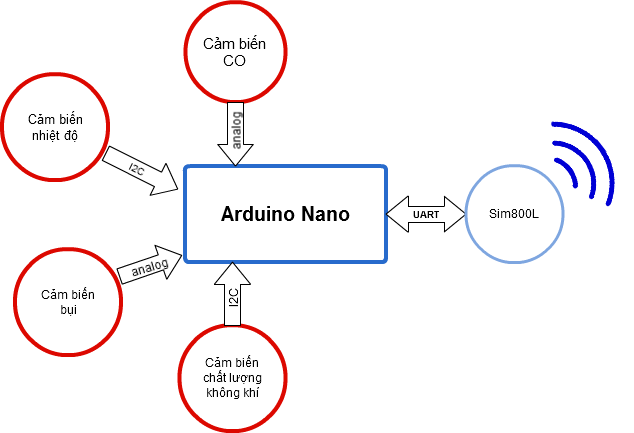
\includegraphics[width=5in]{prototype_1}
	\caption[Mô hình prototype đầu tiên]{Mô hình prototype đầu tiên}
	\label{fig:prototype_1}
\end{figure}
Ngoài những cảm biến đã đề cập thì sơ đồ hoạt động của các khối chức năng trong Hình \ref{fig:prototype_1} còn có thêm những khối chính sau:
\begin{itemize}
	\item[•] Khối Arduino Nano: mạch xử lý trung tâm có nhiệm vụ định thời và điều khiển các khối cảm biến khác để thu thập dữ liệu cảm biến sau đó sẽ xử lý các số liệu thô sang số liệu chính xác, cuối cùng gửi dữ liệu đã được xử lý lên cho máy chủ thông qua khối Sim800L.
	\item[•] Khối Sim800L: chức năng mở kết nối TCP tới máy chủ thông qua dịch vụ GPRS của nhà mạng cung cấp và đưa các dữ liệu từ mạch vi xử lý gửi thông qua giao thức UART.
\end{itemize}



\subsubsection*{Mô hình khối nguồn cho node cảm biến}
Tiếp đến phần thiết kế thì để có thể tận dụng nguồn năng lượng mặt trời để nạp pin cho mạch hoạt động độc lập với điện lưới thì chúng tôi đã đề xuất mô hình khối nguồn như sau:
\begin{figure}[H]
	\centering    
	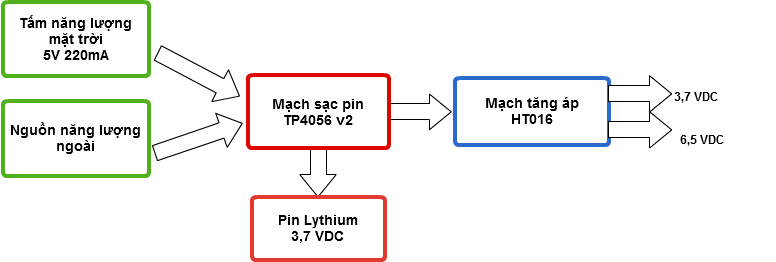
\includegraphics[width=6in]{khoinguon}
	\caption[Mô hình khối nguồn]{Mô hình khối nguồn}
	\label{fig:khoinguon}
\end{figure}

\begin{itemize}
	\item[•]Mạch tăng áp mini HT106 là module tăng áp cực kì nhỏ gọn, ngõ vào là cổng mircoUSB. Mạch có khả năng tăng đến 28v tối đa. Dưới đây là một số thông số kỹ thuật:\\
	-	Điện áp vào: 2-24V\\
	-	Điện áp ra: 5-28V\\
	-	Dòng tối đa: 2A đỉnh, dòng liên tục khoảng 1A.\\
	-	Công suất: 6W\\
	-	Hiệu suất: 93%
	\begin{figure}[H]
		\centering    
		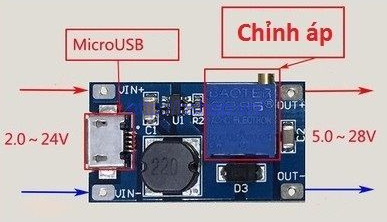
\includegraphics[width=3in]{ht06}
		\caption[Mạch tăng áp mini HT106]{Mạch tăng áp mini HT106}
		\label{fig:ht06}
	\end{figure}
	
	\item[•]Mạch sạc pin Lithium TP4056v2 sử dụng IC quản lý sạc TP4056 nhưng được nâng cấp để có thể ngắt khi pin yếu dưới 2.4V nhằm bảo vệ pin. Một số thông số kỹ thuật của mạch sạc pin Lithium TP4056v2\\
	-	Điện áp đầu vào: 5VDC mini USB\\
	-	Điện áp ngưỡng ra tự động ngắt: 4.2V +- 1%\\
	-	Dòng sạc tối đa: 1000mA\\
	-	Điện áp ngưỡng cần sạc là 2.5V\\
	-	Tích hợp tự động ngắt bảo vệ pin khi pin yếu dưới 2.4 V qua 2 chân OUT+ và OUT-
	\begin{figure}[H]
		\centering    
		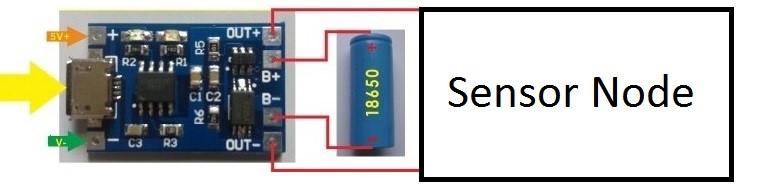
\includegraphics[width=5in]{tp4056}
		\caption[Mạch sạc pin Lithium TP4056v2]{Mạch sạc pin Lithium TP4056v2}
		\label{fig:tp4056}
	\end{figure}
	\item[•]Pin năng lượng mặt trời Poly 5.5V /220 mA\\
	-	Với kích thước: 100x80x2mm\\
	-	Nguồn đầu ra: 5.5V\\
	-	Dòng tối đa cung cấp được: 220mA\\
	\begin{figure}[H]
		\centering    
		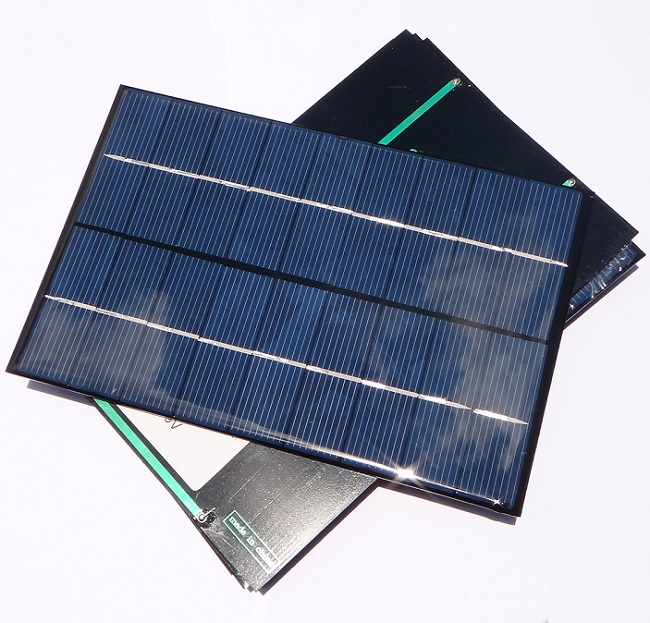
\includegraphics[width=0.6\textwidth]{solarpanel_real}
		\caption[Pin năng lượng mặt trời Poly 5.5V /220 mA]{Pin năng lượng mặt trời Poly 5.5V /220 mA}
		\label{fig:solarpanel_real}
	\end{figure}
	
	\item[•]Nguồn năng lượng ngoài: sử dụng trong một số trường hợp thời tiết mưa nhiều hoặc gió nhiều mà thiếu nguồn năng lượng mặt trời, chúng ta có thể tận dụng nguồn mưa và gió nhờ các tuapin phát năng lượng nhờ vào sức gió và mưa.
	\item[•] Nguồn đầu ra 3.7VDC dùng để cấp cho module Sim800L còn đối với nguồn 6.5VDC dùng để cung cấp cho mạch vi xử lý.
\end{itemize}

\newpage
\subsubsection*{Các thư viện đã sử dụng} 
\begin{lstlisting}[language=C]
#include "MQ135.h" //Thu vien cac ham toan hoc de xu ly so lieu MQ135
#include "MQ07.h" //Thu vien cac ham toan hoc de xu ly so lieu MQ07
#include "OneWire.h" // Thu vien cau hinh giao thuc I2C
#include "DallasTemperature.h" // Thu vien cho cam bien nhiet do
#include "SoftwareSerial.h" // Thu vien mo rong cac chan UART
#include "TimerOne.h" // Thu vien cau hinh timer
\end{lstlisting}



\subsubsection*{Kết quả hiện thực}
\begin{figure}[H]
	\centering    
	\includegraphics[width=5in]{prototype_2}
	\caption[Kết quả prototype đầu tiên]{Kết quả prototype đầu tiên}
	\label{fig:prototype_2}
\end{figure}

\begin{figure}[H]
	\centering    
	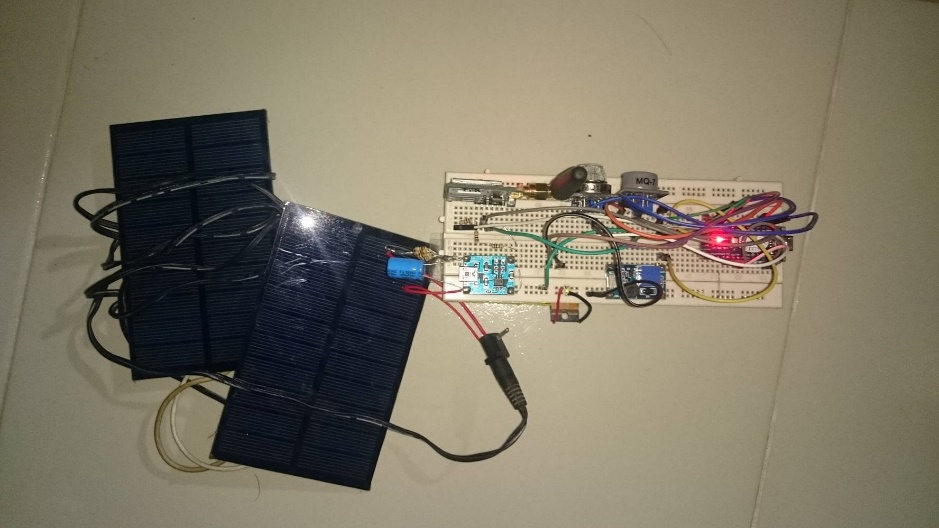
\includegraphics[width=5in]{prototype_3}
	\caption[Kết quả prototype đầu tiên 2]{Kết quả prototype đầu tiên 2}
	\label{fig:prototype_3}
\end{figure}



\subsubsection*{Nhận xét}
\begin{itemize}
	\item[•] Hoàn thành các chức năng có thể đọc được các dữ liệu từ cảm biến MQ135, MQ07, DS18B20, và GP2.
	\item[•] Xử lý được dữ liệu thông qua các thư viện do nhà sản xuất cảm biến cung cấp.
	\item[•] Gửi được dữ liệu lên máy chủ thông qua dịch vụ GPRS của Sim800L, hệ thống máy chủ của chúng tôi ban đầu chưa được hoàn thành nên nhờ đến công cụ phát triển IoT Thingspeak thì chúng tôi đã kiểm tra được, xem thêm tại: \url{https://thingspeak.com/channels/157120}
\end{itemize}



\newpage
\subsection{Hiện thực mô hình tổng thể node cảm biến}
\subsubsection*{Hiện thực board mạch vi xử lý}
Board mạch vi xử lý được thiết kế và hiện thực gọn nhất có thể và hỗ trợ các header nối các dây bus đến các cảm biến và module Sim800L. Chúng tôi đã thực hiện thiết kế board mạch vi xử lý như Hình \ref{fig:botrimcu}

\begin{figure}[H]
	\centering  
	\begin{subfigure}[b]{0.5\textwidth}
		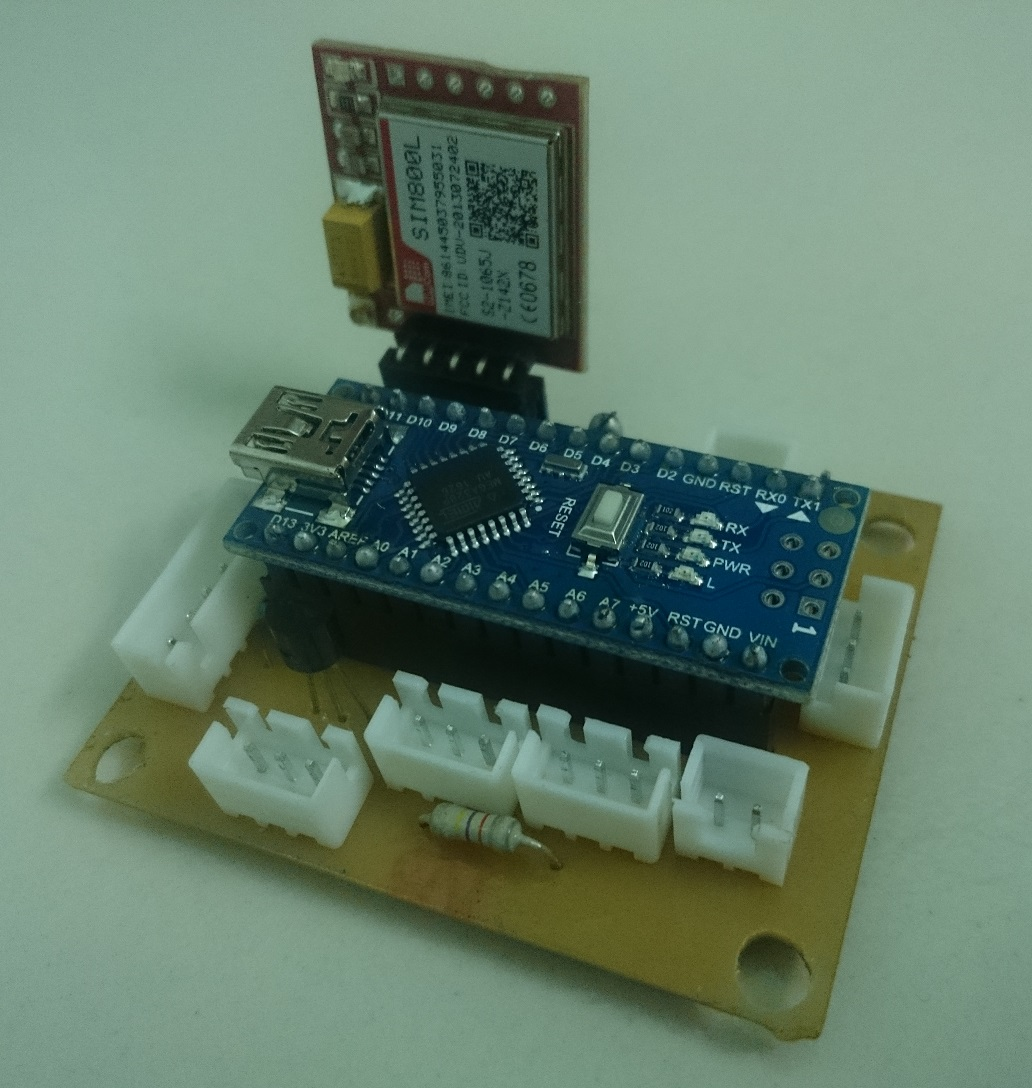
\includegraphics[width=3in]{mcu}
		\caption[Mô hình 1]{Mô hình 1}
		\label{fig:mcu}
	\end{subfigure}\hfill
	\begin{subfigure}[b]{0.5\textwidth}
		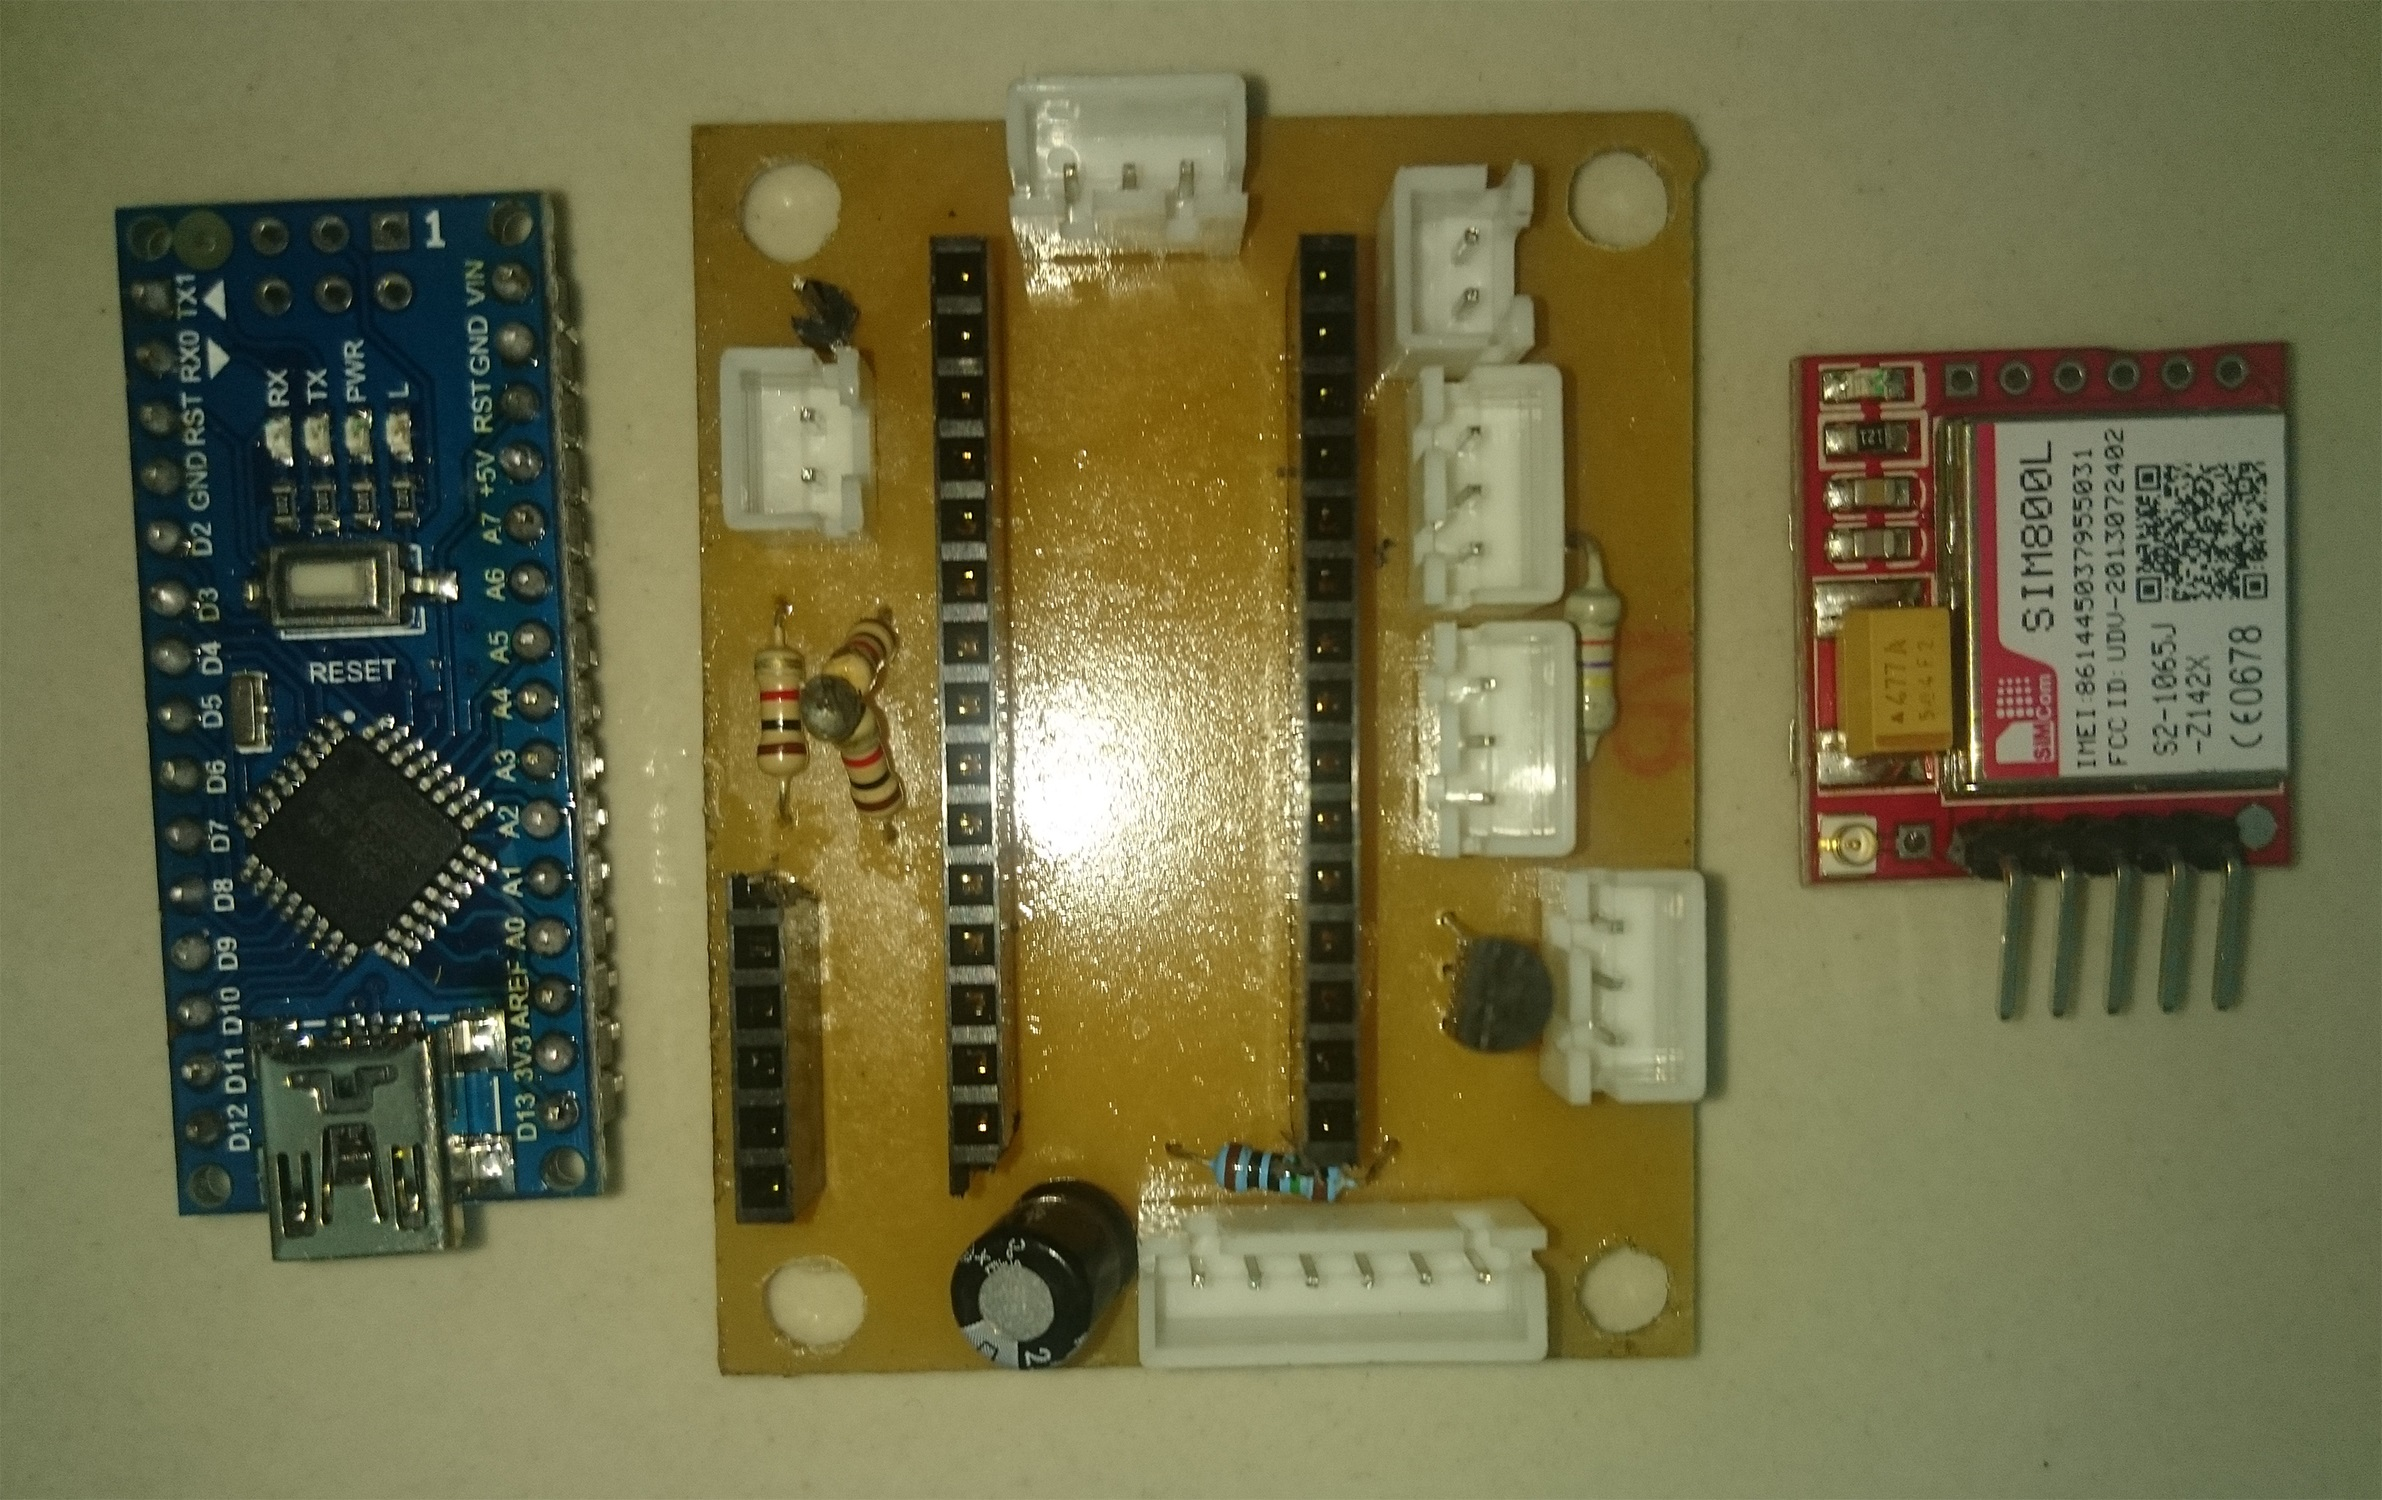
\includegraphics[width=3in]{mcu_2}
		\caption[Mô hình 2]{Mô hình 2}
		\label{fig:mcu_2}
	\end{subfigure}
	\caption{Bố trí board mạch vi xử lý}\label{fig:botrimcu}
\end{figure}

Một số khai báo được sử dụng như sau:
\begin{lstlisting}[numbers=left,firstnumber=1,language=C]
#define ONE_WIRE_BUS 4
#define MQ135_PIN A0
#define MQ7_PIN A1
#define RX_SIM_OUT 11
#define TX_SIM_OUT 10
#define DUST_OUT A2
#define DUST_PIN 2

// Gia tri % Pin thap se khong cho phep mach hoat dong
#define LOW_BATTERY 30 

// So lan gui lai du lieu len may chu neu khong thanh cong
#define TIMEFAIL_SENDSMS 5 

// Mo rong UART tren chan so 11 va 10
SoftwareSerial sim900(RX_SIM_OUT, TX_SIM_OUT);

int TIMEON = 3; //Thoi gian dot nong cam bien MQ135, MQ07

//Thoi gian ngat nguon cam bien MQ135, MQ07 ban ngay
int TIMEOFF_DAY = 13; 
//Thoi gian ngat nguon cam bien MQ135, MQ07 ban dem
int TIMEOFF_NIGHT = 28;

// Moc thoi gian xac dinh buoi sang va buoi toi
int time_s1 = 6;
int time_s2 = 19;

String apiKey = "7"; //Node ID
\end{lstlisting}
Lập trình cho vi xử lý Arduino Nano được mô hình hóa theo lưu đồ xử lý dưới Hình \ref{fig:node_status}:

\begin{figure}[H]
	\centering    
	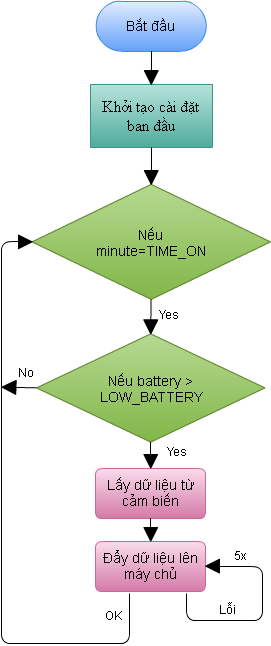
\includegraphics[width=2.5in]{node_status}
	\caption[Lưu đồ xử lý hàm main]{Lưu đồ xử lý hàm main}
	\label{fig:node_status}
\end{figure}

\begin{itemize}
	\item[•]Khởi tạo cài đặt ban đầu gồm các công việc: \\
	- Thiết lập chế độ hoạt động của các chân trên vi xử lý.\\
	- Thiết lập tốc độ truyền UART.\\
	- Thiết lập timer định thời.\\
	- Khởi động Module Sim800L.\\
	- Đồng bộ thời gian module Sim800L với máy chủ NTP.\\
	
	Việc Đồng bộ thời gian module Sim800L với máy chủ NTP được Sim800L hỗ trợ qua các tập lệnh sau:
	\begin{lstlisting}[numbers=left,firstnumber=1,language=C]
	void syncTime()
	{
	//  Network time sync
	sim900.println("AT+SAPBR=1,1");
	delay(2000);
	sim900.println("AT+CNTPCID=1");
	delay(2000);
	sim900.println("AT+CNTP=\"128.4.24.98\",28");
	delay(2000);
	sim900.println("AT+CNTP");
	delay(4000);  
	sim900.println("AT+SAPBR=0,1");
	delay(2000);
	Serial.println("Sync time - Done");
	updateTime();
	}
	\end{lstlisting}
	
	
	
	
	
	
	
\end{itemize}









\subsubsection*{Bố trí các linh kiện trong hộp cảm biến}
Việc bố trí các linh kiện trong hộp cảm biến nhầm giúp cho việc thu thập dữ liệu của các cảm biến được hiệu quả hơn và không bị ảnh hưởng bởi mưa. Nó cũng giúp cho việc phát triển trong tương lai nếu các cảm biến hoặc linh kiện bị hư thì dễ dàng thay thế hơn.

Đối với các cảm biến MQ135, MQ07 và cảm biến nhiệt DS18B20 thì được bố trí đặt ở lớp dưới của chiếc hộp như Hình \ref{fig:botri}

\begin{figure}[H]
	\centering  
	\begin{subfigure}[b]{0.5\textwidth}
		
\includegraphics[width=2.5in]{house_sensor}
		\caption[Mô hình]{Mô hình}
		\label{fig:house_sensor}
	\end{subfigure}\hfill
	\begin{subfigure}[b]{0.5\textwidth}
		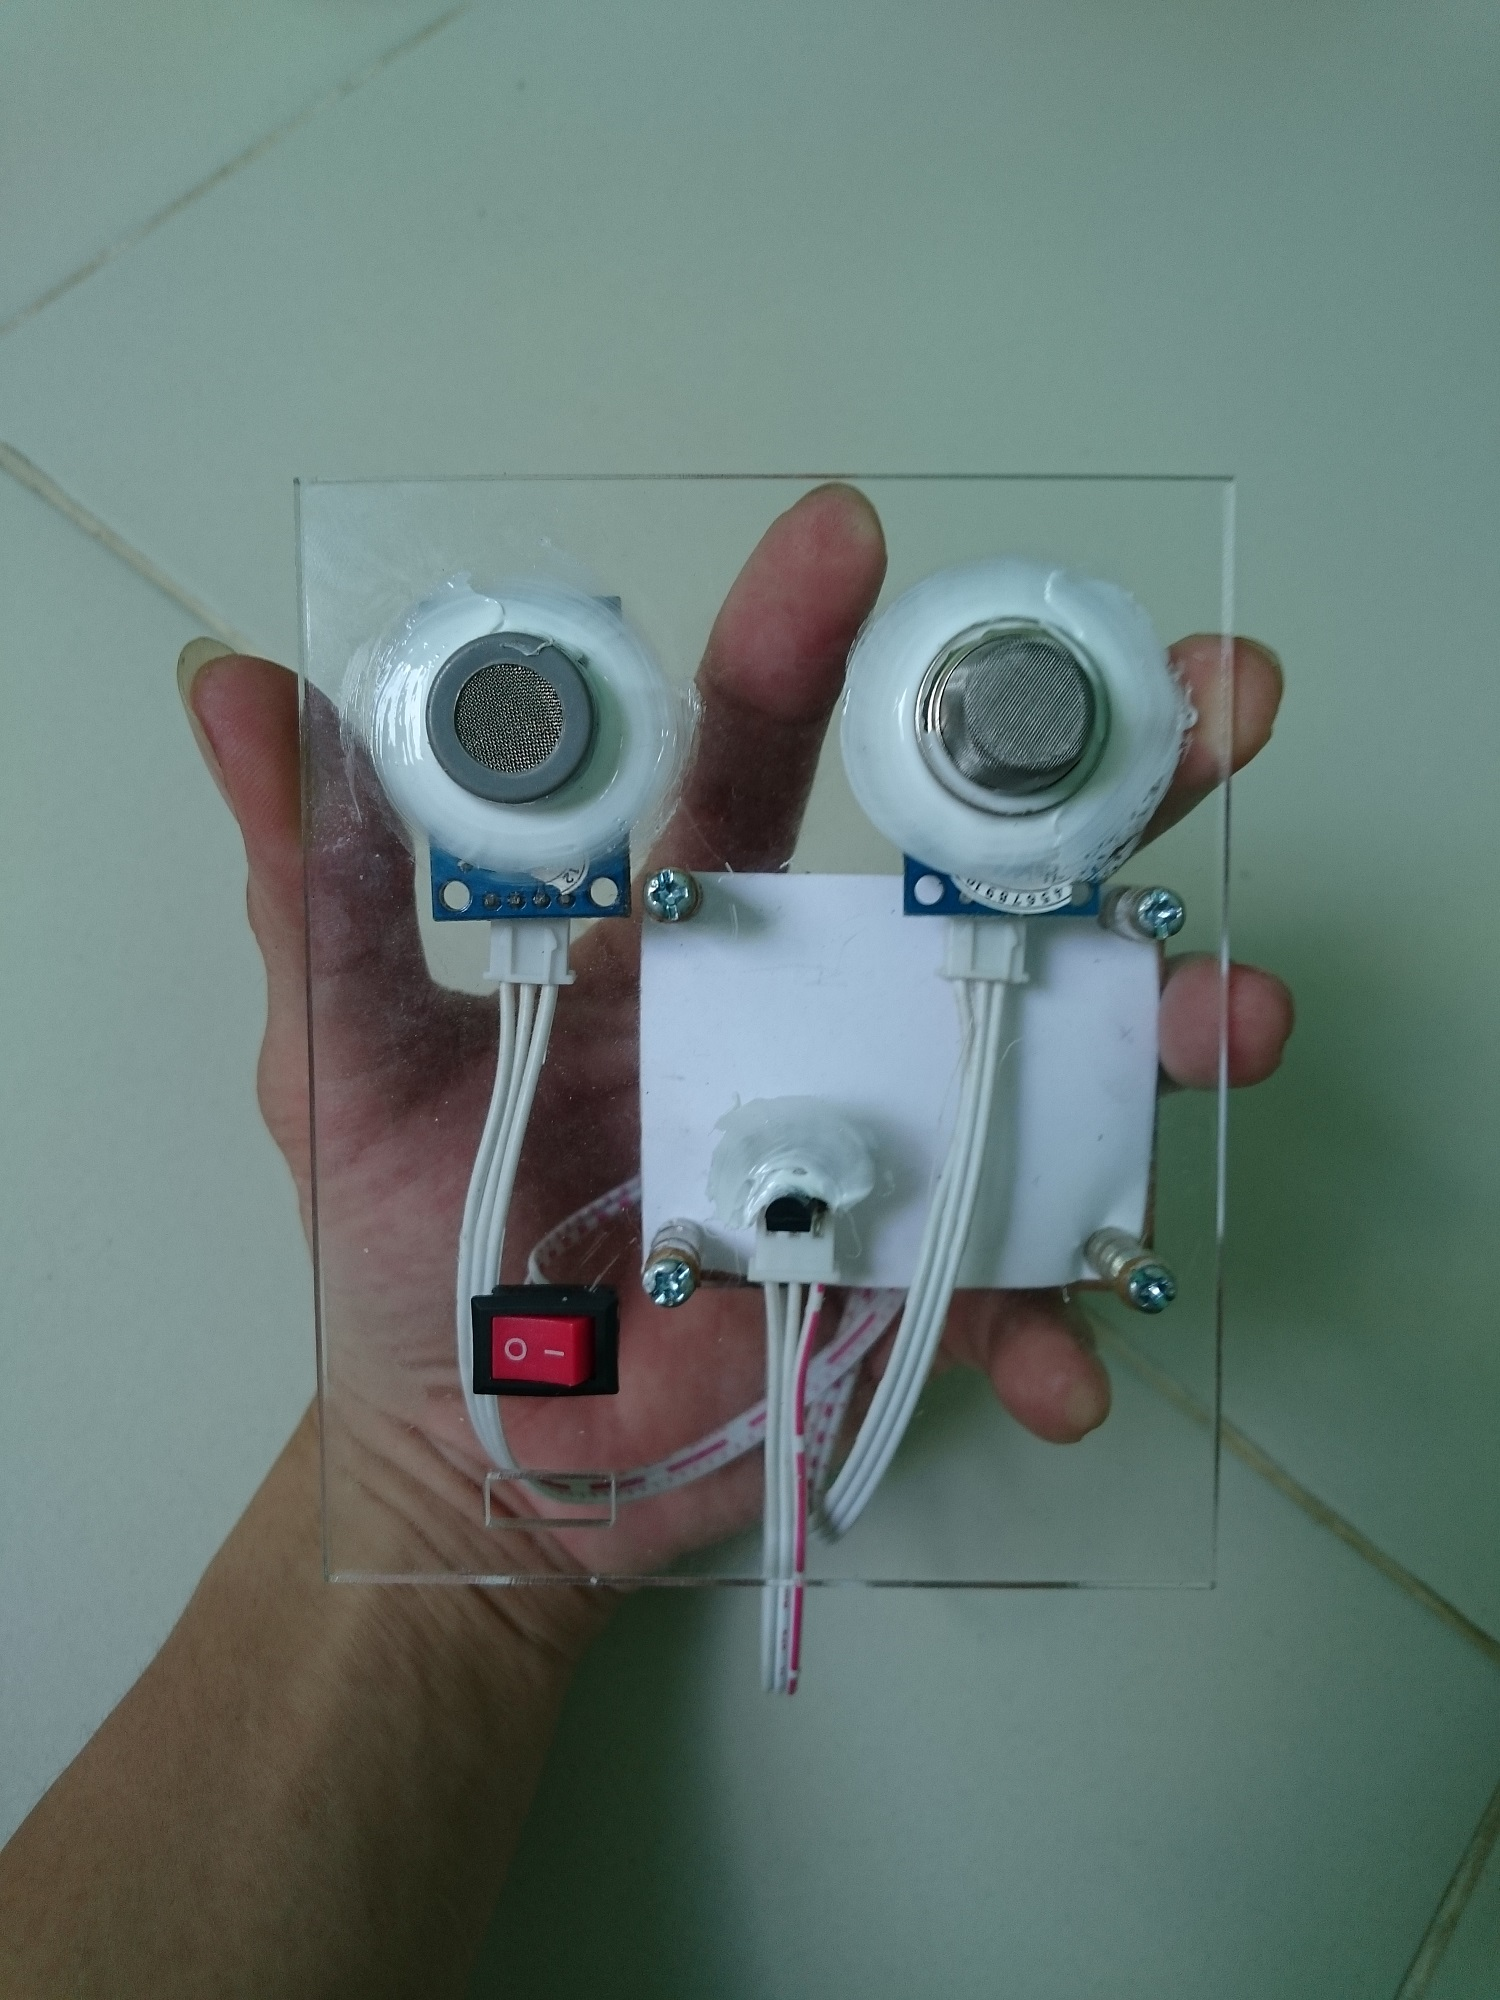
\includegraphics[width=2.5in]{house_sensor_2}
		\caption[Thực tế]{Thực tế}
		\label{fig:house_sensor_2}
	\end{subfigure}
	\caption{Bố trí các cảm biến}\label{fig:botri}
\end{figure}
Đối với các cảm biến bụi GP2 chúng tôi đề xuất vị trí được đặt như Hình \ref{fig:house_dust} sau:
\begin{figure}[H]
	\centering    
	\includegraphics[width=2.5in]{house_dust}
	\caption[Mô hình đặt cảm biến GP2]{Mô hình đặt cảm biến GP2}
	\label{fig:house_dust}
\end{figure}
Còn các board mạch vi xử lý, module Sim800L và pin được đặc vị trí bên trong chiếc hộp như Hình \ref{fig:botrikhac} sau:
\begin{figure}[H]
	\centering  
	\begin{subfigure}[b]{0.5\textwidth}
		\includegraphics[width=2.5in]{house_board_kogps}
		\caption[Mô hình]{Mô hình}
		\label{fig:house_board_kogps}
	\end{subfigure}\hfill
	\begin{subfigure}[b]{0.5\textwidth}
		\includegraphics[width=2.5in]{pic1}
		\caption[Thực tế]{Thực tế}
		\label{fig:pic1}
	\end{subfigure}
	\caption{Bố trí các cảm biến khác}\label{fig:botrikhac}
\end{figure}
\subsection{Mức độ tiêu hao năng lượng}
Để biết được mức tiêu hao năng lượng của mạch hoạt động như thế nào thì chúng tôi đã bắt đầu tính toán từ những thông số tiêu thụ chuẩn của các linh kiện được sử dụng trong node cảm biến. Nhầm nắm bắt được và đưa ra dung lượng pin cần thiết cho các node cảm biến chạy mà không phụ thuộc vào mạng lưới điện.

Chú ý: các thông số tính toán dưới lấy từ thông số chuẩn của nhà sản xuất kèm với một số thông số chuẩn của chúng tôi như sau:
\begin{itemize}
	\item[•] Thời gian cho việc đốt nóng cảm biến MQ135 và MQ07 trước khi lấy dữ liệu: 3 phút
	\item[•] Ban ngày từ 7AM-8PM: cứ mỗi 15 phút gửi dữ liệu lên máy chủ.
	\item[•] Ban đêm từ 8PM-7AM: cứ mỗi 30 phút gửi dữ liệu lên máy chủ.
\end{itemize}

\textbf{Mức tiêu hao năng lượng vào 1 buổi sáng 7AM-8PM:}
\begin{table}[H]
	\centering
	\caption{Bảng tiêu thụ năng lượng buổi sáng}
	\label{table:buoisang}
	\begin{tabular}{|l|l|r|r|r|r|}
		\hline
		\textbf{STT}  & \textbf{Module}                                                       & \multicolumn{1}{c|}{\textbf{\begin{tabular}[c]{@{}c@{}}Dòng tiêu \\ thụ (mA)\end{tabular}}} & \multicolumn{1}{c|}{\textbf{\begin{tabular}[c]{@{}c@{}}Giờ hoạt \\ động (h)\end{tabular}}} & \multicolumn{1}{c|}{\textbf{\begin{tabular}[c]{@{}c@{}}Tổng dòng \\ tiêu thụ(mA)\end{tabular}}} & \multicolumn{1}{c|}{\textbf{\begin{tabular}[c]{@{}c@{}}Công suất\\ (mW)\end{tabular}}} \\ \hline
		1             & Cảm biến bụi                                                          & 20                                                                                          & 13                                                                                         & 260                                                                                             & 858                                                                                    \\ \hline
		2             & Cảm biến MQ07                                                         & 250                                                                                         & 2.6                                                                                        & 650                                                                                             & 3250                                                                                   \\ \hline
		3             & Cảm biến MQ135                                                        & 300                                                                                         & 2.6                                                                                        & 780                                                                                             & 3900                                                                                   \\ \hline
		4             & \begin{tabular}[c]{@{}l@{}}Cảm biến nhiệt độ\\ 18BS20\end{tabular}    & 1.5                                                                                         & 13                                                                                         & 19.5                                                                                            & 97.5                                                                                   \\ \hline
		5             & \begin{tabular}[c]{@{}l@{}}Module Sim800L \\ (idea mode)\end{tabular} & 10                                                                                          & 12.35                                                                                      & 123.5                                                                                           & 456.95                                                                                 \\ \hline
		6             & \begin{tabular}[c]{@{}l@{}}Module Sim800L\\ (Hoạt động)\end{tabular}  & 500                                                                                         & 0.65                                                                                       & 325                                                                                             & 1202.5                                                                                 \\ \hline
		7             & Arduino nano                                                          & 10                                                                                          & 13                                                                                         & 130                                                                                             & 780                                                                                    \\ \hline
		\textbf{Tổng} & \textbf{}                                                             & \textbf{1091.5}                                                                             & \textbf{}                                                                                  & \textbf{2288}                                                                                   & \textbf{10544.95}                                                                      \\ \hline
	\end{tabular}
\end{table}

\textbf{Mức tiêu hao năng lượng vào 1 buổi tối 8PM-7AM:}
\begin{table}[H]
	\centering
	\caption{Bảng tiêu thụ năng lượng buổi tối}
	\label{table:buoitoi}
	\begin{tabular}{|l|l|r|r|r|r|}
		\hline
		\textbf{STT}  & \textbf{Module}                                                       & \multicolumn{1}{c|}{\textbf{\begin{tabular}[c]{@{}c@{}}Dòng tiêu \\ thụ (mA)\end{tabular}}} & \multicolumn{1}{c|}{\textbf{\begin{tabular}[c]{@{}c@{}}Giờ hoạt \\ động (h)\end{tabular}}} & \multicolumn{1}{c|}{\textbf{\begin{tabular}[c]{@{}c@{}}Tổng dòng \\ tiêu thụ(mA)\end{tabular}}} & \multicolumn{1}{c|}{\textbf{\begin{tabular}[c]{@{}c@{}}Công suất\\ (mW)\end{tabular}}} \\ \hline
		1             & Cảm biến bụi                                                          & 20                                                                                          & 11                                                                                         & 220                                                                                             & 726                                                                                    \\ \hline
		2             & Cảm biến MQ07                                                         & 250                                                                                         & 2.2                                                                                        & 550                                                                                             & 2750                                                                                   \\ \hline
		3             & Cảm biến MQ135                                                        & 300                                                                                         & 2.2                                                                                        & 660                                                                                             & 3300                                                                                   \\ \hline
		4             & \begin{tabular}[c]{@{}l@{}}Cảm biến nhiệt độ\\ 18BS20\end{tabular}    & 1.5                                                                                         & 11                                                                                         & 16.5                                                                                            & 82.5                                                                                   \\ \hline
		5             & \begin{tabular}[c]{@{}l@{}}Module Sim800L \\ (idea mode)\end{tabular} & 10                                                                                          & 10.45                                                                                      & 104.5                                                                                           & 386.65                                                                                 \\ \hline
		6             & \begin{tabular}[c]{@{}l@{}}Module Sim800L\\ (Hoạt động)\end{tabular}  & 500                                                                                         & 0.55                                                                                       & 275                                                                                             & 1017.5                                                                                 \\ \hline
		7             & Arduino nano                                                          & 10                                                                                          & 11                                                                                         & 110                                                                                             & 660                                                                                    \\ \hline
		\textbf{Tổng} & \textbf{}                                                             & \textbf{1091.5}                                                                             & \textbf{}                                                                                  & \textbf{1936}                                                                                   & \textbf{8922.65}                                                                       \\ \hline
	\end{tabular}
\end{table}

\section{Hệ thống Server lưu trữ dữ liệu và cung cấp API}

\subsection{Cấu trúc tổ chức tập tin}
\subsubsection*{Các thư mục và chức năng}
Chúng ta có những thư mục được làm việc trực tiếp:

• \textbf{libs}: chứa các hàm function hỗ trợ về xác thực và log.

• \textbf{models}: thư mục này bao gồm các mô hình quản lý cơ sở dữ liệu.

• \textbf{routes}: điều khiển và điều hướng theo các url.

• \textbf{log}: chứa các file ghi lại log trong quá trình hoạt động.

• \textbf{views}: là bộ mặt của web server, giúp người dùng có thể tương tác được với server qua web browser, bao gồm các file giao diện như html, ejs...   


\subsubsection*{Các file khởi tạo và cấu hình Server}

\textbf{Các file khởi tạo này bao gồm:}

• \textbf{emap.js}: file có chức năng đọc file cấu hình và khởi tạo kết nối server.
\begin{lstlisting}[caption=emap.js]
...
server.on('listening', onListening); // open for listening
function onListening() {
var addr = server.address();
var bind = typeof addr === 'string' ?
'pipe' + addr :
'port' + addr.port;
debug('Listening on ' + bind);
console.log('Listening on ' + bind);
};
...
\end{lstlisting}

• \textbf{app.js}: là file điều khiển và thiết lập các chức năng, khai báo các modules chính được sử dụng. Bên cạnh đó, còn có chức năng gán điều hướng tới các file trong thư mục route
\begin{lstlisting}[caption=app.js]
...
// initial server
app.use(passport.initialize());
app.use(passport.session());
app.set('views', path.join(\_\_dirname, 'views'));
app.engine('ejs', engine);
...
// control route
app.use(logger('dev'));
app.use('/log', express.static(path.join(__dirname, 'log')));
app.use(express.static(path.join(__dirname, 'public')));
app.use('/log', serveIndex('./log'));
app.use('/', routes);
app.use('/user', user);
app.use('/node', node);
app.use('/auth', auth);
...
\end{lstlisting}

\textbf{Các file cấu hình này bao gồm:}

• \textbf{package.json}: khai báo các thông tin cơ bản về project và các modules được sử dụng.
\begin{Verbatim}[xleftmargin=2em]
{
"name": "emap-server",
"version": "1.0.0",
"description": "This is serverside part of IoT project",
"main": "emap.js",
"author": "Cuong, Tung and Ny",
"license": "ISC",
"homepage": "www.codingyourfuture.com",
"dependencies": {// dependancies modules
"angular-chart.js": "^1.0.3",
"asyncawait": "^1.0.6",
"babel": "^6.5.2",
"ejs": "^2.5.2",
...
"rethinkdb": "^2.3.3",
"serve-index": "^1.8.0",
"socket.io": "^1.5.0",
}
}
\end{Verbatim}
• \textbf{config.json}: khai báo các thông số cấu hình được sử dụng. Tại đây ta cấu hình thông số kết nối tới RethinkDB và port ứng dụng server nodejs.
\begin{Verbatim}[xleftmargin=2em]
{
"app":{
"port": "8888"
},
"rethinkdb":{
"host": "localhost",
"port" : "28015",
"db": "emap",
"address":"localhost:28015",
"tableList":["nodeData","nodeList","user"]
}
}

\end{Verbatim}


%% Thiết kế API



\subsection{Xây dựng Database}
% TODO: node cảm biến hay sensor node?
Hệ quản lý cơ sở dữ liệu được sử dụng tại hệ thống là RethinkDB như mô hình thiết kế hệ thống tại mục \ref{sec:struc} . Cơ sở dữ liệu được chia làm 3 bảng: nodeList, nodeData và user được miêu tả tại các hình \ref{fig: dbnode} và\ref{fig: dbuser}

Các dữ liệu về node được chia làm hai bảng:

• nodeList: chứa các thông tin về các sensor node, trong đó data\_id đóng vai trò tương tự như foreign key của bảng nodeData để có thể truy xuất dữ liệu.

• nodeData: tập trung những dữ liệu thu thập được từ các sensor node theo thời gian thực. 
\begin{figure}[H]
	\centering    
	\includegraphics[width=1.0\textwidth]{dbnode}
	\caption[Mô hình cấu trúc dữ liệu của Sensor Node]{Mô hình cấu trúc dữ liệu của Sensor Node}
	\label{fig: dbnode}
\end{figure}
Về phía user, chỉ có một bảng quản lý người dùng bao gồm các thông tin cơ bản để xác thực và quyền thay đổi chỉnh sửa dữ liệu sensor node.
\begin{figure}[H]
	\centering    
	\includegraphics[width=0.45\textwidth]{dbuser}
	\caption[Mô hình cấu trúc dữ liệu của User]{Mô hình cấu trúc dữ liệu của User}
	\label{fig: dbuser}
\end{figure}

Vì mục hệ thống phát triển dừng ở mức xây dựng và thiết kế hệ thống thu thập và truy vấn dữ liệu từ các sensor node nên chưa có bảng phân quyền sở hữu giữa người dùng và sensor node.
\subsection{Hiện thực API}
Dựa trên mô hình thiết kế API tại \ref{sec: api}, API được hiện thực và phát triển.


\subsubsection*{API đăng ký và xác thực người dùng}

Các API này được xây dựng để quản lý và phân quyền người dùng, cho phép sử dụng các API về quản lý thông tin của các sensor node.

\textbf{Đăng nhập:}

Hệ thống sử dụng module Passport chạy trên nền Nodejs, có chức năng dễ dàng thiết lập xác thực người dùng. Module này có thể liên kết với các tài khoản phổ biến như Facebook, Google, Twitter... để hỗ trợ phương thức đăng nhập tiện lợi nhất cho người dùng. Tuy nhiên hệ thống chỉ sử dụng phương thức đăng nhập và quản lý người dùng ở mức local vì là phương thức phù hợp với đề tài.

Chi tiết API đăng nhập:
\begin{Verbatim}[xleftmargin=2em]
POST: /auth/login
data: {username,password}
======================
RESPOND:
case Success:
{
code: 1,
username,
message: 'Login successful'
}
case Failure	
{
code: 0,
message: "Invalid username or password"
}
======================
\end{Verbatim}

\textbf{Lưu thông tin người dùng bằng session:}

Sau khi đăng nhập, một session, còn gọi là phiên làm việc, sẽ được hình thành và lưu trữ trong thời gian nhất định. Session cho phép người dùng có thể vào các trang quản lý với quyền hạn cho phép mà không yêu cầu đăng nhập lại, cũng như được phép sử dụng các API quản lý sensor node.

Session sẽ tự động xóa sau một thời gian quy định, cụ thể ở hệ thống này là 10 ngày kể từ lần đăng nhập gần nhất. Người dùng có thể xóa thủ công bằng cách đăng xuất qua phương thức:
\begin{Verbatim}[xleftmargin=2em]
GET: /auth/logout
======================
RESPOND:
case Success:
{
code: 1,
message: "User has logged out"
}
case Failure:	
{
code: 0,
message: "User has not logged in yet"
}	
\end{Verbatim}

Quá trình đăng nhập và tạo session được mô tả như hình \ref{fig: apilogin}

\begin{figure}[H]
	\centering    
	\includegraphics[width=1\textwidth]{apilogin}
	\caption[Quá trình đăng nhập và tạo session]{Quá trình đăng nhập và tạo session}
	\label{fig: apilogin}
\end{figure}


\textbf{Đăng ký:}

\begin{Verbatim}[xleftmargin=2em]
POST: /user/register
data:{username, password, name, mail}
======================	
RESPOND:
{
code: -1,
message: "Username existed"
}
{
code: -2,
message: "Mail is used",
}
{
code: 1,
message: "Account created successful"
}
======================	
\end{Verbatim}
\subsubsection*{API cung cấp và quản lý sensor node}
Các API được miêu tả tại bảng \ref{table: apilist}, các request và respond được miêu tả chi tiết:

• API thiết lập và cấu hình các sensor node: initnew, updatenode và replace node yêu cầu phải có đăng nhập từ API xác thực người dùng để giữ session và sau đó mới có thể sử dụng. Các API này có cấu trúc tương tự nhau và được mô tả:
\begin{Verbatim}[xleftmargin=2em]
POST: /node/initnew
data: {node_id,lat,lng,phone,status}
======================
RESPOND:
case Success:
{
code: 1,
message: 'Add node successful'
}
case Duplicated:
{
code: 0,
message: 'Node duplicated'
}
case Failure:
{
code: 0,
message: 'Add node failure'
}
case Not authenticated:
{
code: -1,
message: 'You are not authenticated'
}
======================	

\end{Verbatim}
Quá trình đăng nhập và tạo session được mô tả như hình \ref{fig: apipost}

\begin{figure}[H]
	\centering    
	\includegraphics[width=1\textwidth]{apipost}
	\caption[Quá trình kiểm tra session của API POST]{Quá trình kiểm tra session của API POST}
	\label{fig: apipost}
\end{figure}

• API get thông tin và dữ liệu các sensor node: sử dụng phương thức GET để truy xuất dữ liệu về thông tin sensor node và dữ liệu các cảm biến. Hệ thống được thiết kế mang tính mở và chia sẻ nên không yêu cầu đăng nhập để truy xuất dữ liệu. Các thông tin đặc tả chi tiết API:
\begin{Verbatim}[xleftmargin=2em]
GET:	/node/getinfo?*query
Ex: 	/node/getinfo?id=1&status=0
/node/getinfo?list=1&status=1
Query:
+ id=*node ID* để get node bằng ID
+ phone: *node phonenumber* để get node bằng phone number
+ list=1 để get list các node
+ status=1 để get node đang ở trạng thái active,= 0 để node ở tất cả 
trạng thái, cũng như lịch sử thay đổi node
======================
RESPOND:
data:
- single node:{node_id,location:{lat,lng},phone,,time,data_id,status}
- list: array of {node_id,location:{lat,lng},phone,time,data_id,status}
======================
\end{Verbatim}

• API push dữ liệu từ sensor node: cũng tương tự như API get dữ liệu, API push dữ liệu sử dụng method GET thay cho POST để hỗ trợ dễ dàng trong việc thiết lập các thiết bị IoT đóng góp dữ liệu. Lượng dữ liệu của các sensor node không quá lớn, chỉ bao gồm những trường sensor ID và node ID nên có thể tích hợp vào thanh header của request.

\begin{Verbatim}[xleftmargin=2em]
GET: 	/node/pushdata?*query
Ex: 	/node/pushdata?node_id=1&s1=22&s2=33&s3=44&s4=55&s5=66
Query:
+ node_id: node ID
+ s1,s2,s3,s4,s5: value of each sensor
======================
RESPOND:
case Success:
{
code: 1,
message: 'Add node data successful'
}
case Failure:	
{
code: 0,
message: 'Add node data failure'
}
======================
\end{Verbatim}

\subsubsection*{Cung cấp API log}

Để hỗ trợ bên nhà phát triển thứ ba ứng dụng API tốt hơn, hệ thống có cung cấp các thông tin hoạt động của server, các request và respond cũng như các dữ liệu được truy vấn. Khi truy cập vào đường dẫn /log/, chúng ta sẽ có những file log tương ứng với các ngày như hình \ref{fig: log} :

\begin{figure}[H]
	\centering    
	\includegraphics[width=1.0\textwidth]{log}
	\caption[Hiển thị các file log]{Hiển thị các file log}
	\label{fig: log}
\end{figure}

Ví dụ cụ thể của một đoạn log:
\begin{lstlisting}
{"level":"info","message":"IP:123.151.42.61 GET /route","timestamp":"10:48:56"}
{"level":"info","message":"IP:14.161.14.94 GET /statis route","timestamp":"10:49:22"}
{"level":"info","message":"IP:14.161.14.94 GET /graph route","timestamp":"10:49:27"}
{"level":"info","message":"IP:14.161.14.94 GET /node/getinfo: get list node info - number of nodes 12","timestamp":"10:49:27"}
{"level":"info","message":"IP:14.161.14.94 GET /node/getinfo: get node info by id:9","timestamp":"10:49:29",{"data_id":"106c59fe-753d-4a76-8418-88fd0df68d0c","id":"87b7f859-8c1e-4608-9645-5105ebb38e9b", "location":{"lat":10.91085286140159,"lng":106.99790954589844}, "node_id":"9","phone":"0123456899","status":1,"time":"2016-12-06T02:08:57.943Z"}}
{"level":"info","message":"IP:14.161.14.94 GET /node/getdata: Node data ID 9 number of records:  120","timestamp":"10:49:29"}
\end{lstlisting}

Các thông tin được thể hiện trong file log đủ thông tin để cho phép nhà phát triển theo dõi và áp dụng trong việc hiện thực sản phẩm.
\subsection{Xây dựng Web Server}

\subsection{Hiện thực giao diện}

Sử dụng framework express của Nodejs và HTML để xây dựng frontend

\subsubsection*{Giao diện chính của Web Server}
Phần này chứa các nút menu chức năng cùng với google map để theo dõi vị trí hoạt động của các cảm biến.
\begin{center}
	\begin{figure}[H]
		\centering    
		\includegraphics[width=1\textwidth]{webserver}
		\caption[Giao diện chính của Web Server]{Giao diện chính của Web Server}
		\label{fig:webserver}
	\end{figure}
\end{center}

\subsubsection*{Giao diện đồ thị dữ liệu}
Là nơi hiện thị biểu đồ của các thông số cũng như thông tin tương ứng của các cảm biến.
\begin{center}
	\begin{figure}[H]
		\centering    
		\includegraphics[width=1\textwidth]{web_graph}
		\caption[Giao diện đồ thị dữ liệu]{Giao diện đồ thị dữ liệu}
		\label{fig:web_graph}
	\end{figure}
\end{center}



\subsubsection*{Giao diện nhận feedback từ người dùng qua email}
Tương tác giữa người dùng với người quản lý server. Nội dung được gửi thông qua gmail.
\begin{center}
	\begin{figure}[H]
		\centering    
		\includegraphics[width=1\textwidth]{web_email}
		\caption[Giao diện nhận feedback người dùng]{Giao diện nhận feedback người dùng}
		\label{fig:web_email}
	\end{figure}
\end{center}

\subsubsection*{Giao diện dành cho người quản lý}
Khu vực này dành cho người quản lý truy cập nhầm mục đích chỉnh sửa, thay thế các node cảm biến.
\begin{center}
	\begin{figure}[H]
		\centering    
		\includegraphics[width=1\textwidth]{web_nodeinfo}
		\caption[Giao diện quản lý các node cảm biến]{Giao diện quản lý các node cảm biến}
		\label{fig:web_nodeinfo}
	\end{figure}
\end{center}






\newpage
\section{Ứng dụng thiết bị di động}
\subsection{Hiện thực giao diện và chức năng}
\subsubsection*{Giao diện chính ứng dụng di động}
Tại giao diện chính của ứng dụng di động người dùng có thể xem được danh sách thông tin chi tiết của các node cảm biến có trong hệ thống.
\begin{figure}[H]
	\centering  
	\begin{subfigure}[b]{0.5\textwidth}
		\includegraphics[width=2.5in]{main_1}
		\caption[Giao diện chính]{Giao diện chính}
		\label{fig:main_1}
	\end{subfigure}\hfill
	\begin{subfigure}[b]{0.5\textwidth}
		\includegraphics[width=2.5in]{main_2}
		\caption[Giao diện thanh menu]{Giao diện thanh menu}
		\label{fig:main_2}
	\end{subfigure}
	\caption{Giao diện chính ứng dụng di động}\label{fig:giaodienchinh}
\end{figure}


\subsubsection*{Giao diện xem dữ liệu trên ứng dụng di động}
Giao diện này cho phép người dùng theo dõi được dữ liệu của từng node cảm biến theo 2 loại biểu đồ như Hình \ref{fig:app_graph} thể hiện.
\begin{figure}[H]
	\centering  
	\begin{subfigure}[b]{0.5\textwidth}
		\includegraphics[width=2.5in]{main_4}
		\caption[Giao diện xem dữ liệu]{Giao diện xem dữ liệu}
		\label{fig:main_4}
	\end{subfigure}\hfill
	\begin{subfigure}[b]{0.5\textwidth}
		\includegraphics[width=2.5in]{main_3}
		\caption[Giao diện thống kê]{Giao diện thống kê}
		\label{fig:main_3}
	\end{subfigure}
	\caption{Giao diện ứng dụng di động}\label{fig:giaodienchinh2}
\end{figure}
\section{Tính ổn định của node cảm biến}
\textbf{này nói về mấy tháng đo, gió mưa đồ}

Lorem ipsum dolor sit amet, consectetur adipiscing elit, sed do eiusmod tempor incididunt ut labore et dolore magna aliqua. Ut enim ad minim veniam, quis nostrud exercitation ullamco laboris nisi ut aliquip ex ea commodo consequat. Duis aute irure dolor in reprehenderit in voluptate velit esse cillum dolore eu fugiat nulla pariatur. Excepteur sint occaecat cupidatat non proident, sunt in culpa qui officia deserunt mollit anim id est laborum
\section{Đánh giá Server}
\subsection{Tính sẵn sàng}
\begin{itemize}
\item[•] Hiện thực đoạn mã tự động khởi dộng Server khi nguồn điện có lại sau khi bị mất điện.\
\item[•] Sử dụng dịch vụ Dynamic DNS NOIP để cấu hình động tên miền gán với địa chỉ IP của Server tên miền hoạt động lại ngay sau khi vừa thay đổi địa chỉ IP(khắc phục sự cố mất điện làm IP thay đổi).
\end{itemize}
\subsection{Tính ổn định}
\begin{itemize}
	\item[•]Thực tế từ ngày khởi tạo Server và cho hoạt động liên tục 24/7 tới thời gian viết báo cáo là 8 tuần không có lỗi lạ xảy ra (trừ các trường hợp đặc biệt như mất điện, mạng mất kết nối)
	\item[•]Điện năng tiêu thụ thấp và nhiệt độ không quá cao, giao động (44 - 48 độ C) đảm bảo tốt trạng thái hoạt động.
\end{itemize}
\subsection{Tốc độ đáp ứng}
\begin{itemize}
	\item[•] Với sức mạnh của Raspberry Pi 3 thì Server hoạt đông tốt, thời gian tải file giao diện web nhanh với độ trễ thấp < 1s. Thời gian đáp ứng trung bình vào khoảng dưới 100ms là tải xong các tập tin giao diện web được gửi từ Server tới client.
	\item[•] Dịch vụ Google Maps hoạt động khá nhanh mặc dù gói tin truyền đi là chậm nhất vì lượng dữ liệu lớn.
	\item[•] API đáp ứng tốt, nhanh và hiệu quả. Thử nghiệm lập trình ứng dụng di động sử dụng API có thời gian đáp ứng tốt.
\end{itemize}

\section{Đánh giá lập trình ứng dụng Mobile sử dụng APIs}
\begin{itemize}
\item[•]Ứng dụng được viết có thể được xài trên nhiều platforms.
\item[•]Đã hiện thực được file APK cho mobile.
\item[•]Xây dựng một số các chức năng cơ bản như: hiện thị thông tin các node cảm biến cho màn hình chính, vẽ đồ thị, liên kết với web browser …
\item[•] Vẫn còn một vài chức năng cần hoàn thiện: đăng nhập quản lý người dùng, các chức năng phụ liên quan đến user …
\item[•] Khó khăn trong việc debugging vì một số plugin hay chức năng không chạy trên nền web app. 
\item[•]Hiệu suất thấp do nó không hoàn toàn tự nhiên, có thể gặp sự cố khi làm ứng dụng game hay các ứng dụng dùng nhiều tài nguyên.

\end{itemize}
\chapter{Tổng kết và Hướng phát triển cho tương lai}

% **************************** Define Graphics Path **************************
\ifpdf
    \graphicspath{{Chapter5/Figs/Raster/}{Chapter5/Figs/PDF/}{Chapter5/Figs/}}
\else
    \graphicspath{{Chapter5/Figs/Vector/}{Chapter5/Figs/}}
\fi

\section{Tổng kết}
\subsection{Kết quả đạt được}

\subsubsection*{Sensor Box}
\begin{itemize}
\item[•] Tìm hiểu được về các thành phần trong khí thải và mức độ ảnh hưởng tới môi trường.
\item[•] Tìm hiểu các loại cảm biến và cách thức hoạt động. 
\item[•] Hiện thực hoàn chỉnh các chức năng module thu thập dữ liệu từ các cảm biến.
\item[•] Thiết kế và hiện thực được Sensor Box có khả năng hoạt động dưới những môi trường nắng, mưa, gió, bụi.
\item[•] Nghiên cứu và tích hợp được thêm module sử dụng năng lượng mặt trời và mạch nạp pin cho phép hệ thống hoạt động độc lập với điện lưới.
\item[•] Thu thập được dữ liệu từ 3 Sensor Node đã hiện thực tại những địa điểm khác nhau trong suốt thời gian gần 2 tháng.
\end{itemize}

\subsubsection*{Server}
\begin{itemize}
\item[•] Cung cấp API và API log cho nhà phát triển.
\item[•] Áp dụng mô hình kiến trúc hệ thống thuận tiện cho phát triển ứng dụng realtime.
\item[•] Xây dựng giao diện trực quan và thân thiện với người dùng, liên kết cơ sở dữ liệu thời gian thực cung cấp thông tin kịp thời để tiện lợi cho quá trình theo dõi và đánh giá.
\item[•] Đồ thị Google Maps và đồ thị dữ liệu cho việc theo dõi các thông số.
\item[•] Giao tiếp thông qua gmail giữa người dùng và người quản lý.
\end{itemize}

\subsubsection*{Ứng dụng thiết bị di động}
\begin{itemize}
\item[•] Sử dụng Framework Ionic xây dựng được ứng dụng di động trên nhiều nền tảng khác nhau.
\item[•] Liên kết ứng dụng với API được cung cấp, thực hiện một số chức năng cơ bản: hiên thị thông tin node, đồ thị, thống kê.
\end{itemize}

\subsection{Những thuận lợi,khó khăn và mặt hạn chế}
\subsubsection*{Thuận lợi}
\begin{itemize}
\item[•] Giáo viên hướng dẫn thường xuyên lên kế hoạch báo cáo 2 tuần một lần để cập nhật tình hình và giúp đỡ nhóm giải quyết những vấn đề khó khăn trong suốt quá trình làm đề tài luận văn.
\item[•] Được hỗ trợ kinh phí từ giáo viên hướng dẫn.
\item[•] Thời tiết nắng, mưa, gió, bụi đầy đủ để có thể thử nghiệm độ hiểu quả của Sensor Box.
\item[•] Được phòng Lab BKIT hỗ trợ về mặt máy móc, kỹ thuật trong suốt quá trình làm luận văn tốt nghiệp.
\end{itemize}

\subsubsection*{Khó khăn}
\begin{itemize}
\item[•] Các module năng lượng mặt trời không có sẵn, phải tìm các module khác để thay thế.
\item[•] Chưa có thiết bị chuẩn để thực hiện quá trình calibration cho các cảm biến.
\item[•] Dành nhiều thời gian để tiếp cận với hướng lập trình phần mềm và công nghệ mới.
\item[•] Thử nghiệm nhiều với các module sim khác nhau.
\item[•] Thiếu các thiết bị di động để thử nghiệm tính đa nền tảng của ứng dụng di động trên các nền tảng iOS, Windows Phone.
\item[•] Dành nhiều thời gian tìm hiểu và làm quen với các công nghệ mới.
\end{itemize}
\subsubsection*{Mặt hạn chế của đề tài luận văn}
\begin{itemize}
\item[•] Việc tích hợp module năng lượng mặt trời và mạch nạp pin chưa thật sự hiệu quả để Sensor Box hoạt động ổn định độc lập với điện lưới, vấn đề được khắc phục trong tương lai nhờ tìm các tấm năng lượng mặt trời khác hoặc các nguồn năng lượng ngoài như: gió, mưa.
\item[•] Chỉ dừng ở mức thu thập và thống kê, chưa phát triển phân tích các thông số môi trường.
\item[•] Cụm server đặt trên Raspberry Pi 3 không đủ sức mạnh đáp ứng số lượng lớn người dùng cùng một lúc.
\item[•] Vẫn còn một số chức năng chưa hoàn thiện: quản lý người dùng cho ứng dụng di động.
\item[•] Chưa hiện thực cơ chế bảo mật mã hóa gói tin.
\item[•] Quá trình calibration chưa được tốt vì chưa có thiết bị chuẩn.
\end{itemize}


\section{Những kiến thức tiếp thu được qua đề tài}
\subsection{Về mặt kiến thức tổng quát}
\begin{itemize}
	\item[•] Nắm bắt được mô hình xây dựng ứng dụng IoT và các hướng phát triển.
	\item[•] Tiếp thu được kiến thức về môi trường và các yếu tố ảnh hưởng.
	\item[•] Làm quen với các chuẩn giao tiếp mới.
	\item[•] Các thức triển khai và thực nghiệm hệ thống.
	\item[•] Củng cố và phát triển khả năng viết và cấu trúc bản báo cáo. 
\end{itemize}
\subsection{Về mặt hiện thực thiết bị}
\begin{itemize}
	\item[•] Ứng dụng tốt việc lập trình với module SIM800L.
	\item[•] Biết cách áp dụng được nguồn pin năng lượng mặt trời vào thiết bị hoạt động thực tế.
	\item[•] Nắm bắt và xử lý được nhiều trường hợp trong quá trình xây dựng Sensor Box.
\end{itemize}
\subsection{Về mặt xây dựng hệ thống Server và ứng dụng}
\begin{itemize}
	\item[•] Mô tả được mô hình cụm Server và phát triển các ứng dụng Web và di động.
	\item[•] Làm quen với thiết kế và xử lý trong hệ cơ sở dữ liệu.
	\item[•] Tìm tòi học hỏi và áp dụng các công nghệ xử lý thời gian thực.
	\item[•] Cải thiện kỹ năng lập trình và thiết kế trong mảng UI(giao diện người dùng) và UX(trải nghiệm người dùng).
	\item[•] Nắm được cách thức phát triển và áp dụng các API.
\end{itemize}
\section{Hướng phát triển tương lai}
\begin{itemize}
	%sensor node here
\item[•] Chuẩn hóa các cảm biến MQ07, MQ135 bằng các thiết bị đo chuẩn để lấy được giá trị chính xác nhất có thể.
\item[•] Tiếp tục hoàn thiện phần Server hoạt động hiệu quả, đáp ứng hoạt động cho một số lượng lớn các node cảm biến.
\item[•] Xây dựng hệ thống quản lý node theo người dùng, đáp ứng nhu cầu quản lý và thống kê theo từng người.
\item[•] Xây dựng thuật toán phân tích dữ liệu môi trường và áp dụng Machine learning trong việc phân tích dữ liệu để đưa ra kết quả dự đoán tính trạng ô nhiễm môi trường và mật độ giao thông.
\item[•] Nghiên cứu và ứng dụng các nguồn thu năng lượng từ gió, mưa cho Sensor Node.
\item[•] Phát triển ứng dụng thiết lập, chỉnh sửa, thay thế Sensor Node dành cho người phát triển thiết bị.
\item[•] Tích hợp module bluetooth để thu thập các dữ liệu người dùng xung quanh Sensor Node.
\item[•] Tích hợp công nghệ nạp và nâng cấp firmware không dây.
\end{itemize}

%\include{Chapter6/chapter6}
%\include{Chapter7/chapter7}



% ********************************** Back Matter *******************************
% Backmatter should be commented out, if you are using appendices after References
%\backmatter

% ********************************** Bibliography ******************************
\begin{spacing}{0.9}

% To use the conventional natbib style referencing
% Bibliography style previews: http://nodonn.tipido.net/bibstyle.php
% Reference styles: http://sites.stat.psu.edu/~surajit/present/bib.htm

\bibliographystyle{apalike}
%\bibliographystyle{unsrt} % Use for unsorted references  
%\bibliographystyle{plainnat} % use this to have URLs listed in References
\cleardoublepage
\bibliography{References/references} % Path to your References.bib file


% If you would like to use BibLaTeX for your references, pass `custombib' as
% an option in the document class. The location of 'reference.bib' should be
% specified in the preamble.tex file in the custombib section.
% Comment out the lines related to natbib above and uncomment the following line.

%\printbibliography[heading=bibintoc, title={References}]


\end{spacing}

%\appendix
%% ******************************* Thesis Appendix A ****************************
\chapter{How to install \LaTeX} 

\section*{Windows OS}

\subsection*{TeXLive package - full version}
\begin{enumerate}
\item	Download the TeXLive ISO (2.2GB) from\\
\href{https://www.tug.org/texlive/}{https://www.tug.org/texlive/}
\item	Download WinCDEmu (if you don't have a virtual drive) from \\
\href{http://wincdemu.sysprogs.org/download/}
{http://wincdemu.sysprogs.org/download/}
\item	To install Windows CD Emulator follow the instructions at\\
\href{http://wincdemu.sysprogs.org/tutorials/install/}
{http://wincdemu.sysprogs.org/tutorials/install/}
\item	Right click the iso and mount it using the WinCDEmu as shown in \\
\href{http://wincdemu.sysprogs.org/tutorials/mount/}{
http://wincdemu.sysprogs.org/tutorials/mount/}
\item	Open your virtual drive and run setup.pl
\end{enumerate}

or

\subsection*{Basic MikTeX - \TeX~ distribution}
\begin{enumerate}
\item	Download Basic-MiK\TeX (32bit or 64bit) from\\
\href{http://miktex.org/download}{http://miktex.org/download}
\item	Run the installer 
\item	To add a new package go to Start >> All Programs >> MikTex >> Maintenance (Admin) and choose Package Manager
\item	Select or search for packages to install
\end{enumerate}

\subsection*{TexStudio - \TeX~ editor}
\begin{enumerate}
\item	Download TexStudio from\\
\href{http://texstudio.sourceforge.net/\#downloads}
{http://texstudio.sourceforge.net/\#downloads} 
\item	Run the installer
\end{enumerate}

\section*{Mac OS X}
\subsection*{MacTeX - \TeX~ distribution}
\begin{enumerate}
\item	Download the file from\\
\href{https://www.tug.org/mactex/}{https://www.tug.org/mactex/}
\item	Extract and double click to run the installer. It does the entire configuration, sit back and relax.
\end{enumerate}

\subsection*{TexStudio - \TeX~ editor}
\begin{enumerate}
\item	Download TexStudio from\\
\href{http://texstudio.sourceforge.net/\#downloads}
{http://texstudio.sourceforge.net/\#downloads} 
\item	Extract and Start
\end{enumerate}


\section*{Unix/Linux}
\subsection*{TeXLive - \TeX~ distribution}
\subsubsection*{Getting the distribution:}
\begin{enumerate}
\item	TexLive can be downloaded from\\
\href{http://www.tug.org/texlive/acquire-netinstall.html}
{http://www.tug.org/texlive/acquire-netinstall.html}.
\item	TexLive is provided by most operating system you can use (rpm,apt-get or yum) to get TexLive distributions
\end{enumerate}

\subsubsection*{Installation}
\begin{enumerate}
\item	Mount the ISO file in the mnt directory
\begin{verbatim}
mount -t iso9660 -o ro,loop,noauto /your/texlive####.iso /mnt
\end{verbatim}

\item	Install wget on your OS (use rpm, apt-get or yum install)
\item	Run the installer script install-tl.
\begin{verbatim}
	cd /your/download/directory
	./install-tl
\end{verbatim}
\item	Enter command `i' for installation

\item	Post-Installation configuration:\\
\href{http://www.tug.org/texlive/doc/texlive-en/texlive-en.html\#x1-320003.4.1}
{http://www.tug.org/texlive/doc/texlive-en/texlive-en.html\#x1-320003.4.1} 
\item	Set the path for the directory of TexLive binaries in your .bashrc file
\end{enumerate}

\subsubsection*{For 32bit OS}
For Bourne-compatible shells such as bash, and using Intel x86 GNU/Linux and a default directory setup as an example, the file to edit might be \begin{verbatim}
edit $~/.bashrc file and add following lines
PATH=/usr/local/texlive/2011/bin/i386-linux:$PATH; 
export PATH 
MANPATH=/usr/local/texlive/2011/texmf/doc/man:$MANPATH;
export MANPATH 
INFOPATH=/usr/local/texlive/2011/texmf/doc/info:$INFOPATH;
export INFOPATH
\end{verbatim}
\subsubsection*{For 64bit OS}
\begin{verbatim}
edit $~/.bashrc file and add following lines
PATH=/usr/local/texlive/2011/bin/x86_64-linux:$PATH;
export PATH 
MANPATH=/usr/local/texlive/2011/texmf/doc/man:$MANPATH;
export MANPATH 
INFOPATH=/usr/local/texlive/2011/texmf/doc/info:$INFOPATH;
export INFOPATH

\end{verbatim}



%\subsection{Installing directly using Linux packages} 
\subsubsection*{Fedora/RedHat/CentOS:}
\begin{verbatim} 
sudo yum install texlive 
sudo yum install psutils 
\end{verbatim}


\subsubsection*{SUSE:}
\begin{verbatim}
sudo zypper install texlive
\end{verbatim}


\subsubsection*{Debian/Ubuntu:}
\begin{verbatim} 
sudo apt-get install texlive texlive-latex-extra 
sudo apt-get install psutils
\end{verbatim}

% ********************************** Appendices ********************************

\begin{appendices} % Using appendices environment for more functunality

%% ******************************* Thesis Appendix A ****************************
\chapter{How to install \LaTeX} 

\section*{Windows OS}

\subsection*{TeXLive package - full version}
\begin{enumerate}
\item	Download the TeXLive ISO (2.2GB) from\\
\href{https://www.tug.org/texlive/}{https://www.tug.org/texlive/}
\item	Download WinCDEmu (if you don't have a virtual drive) from \\
\href{http://wincdemu.sysprogs.org/download/}
{http://wincdemu.sysprogs.org/download/}
\item	To install Windows CD Emulator follow the instructions at\\
\href{http://wincdemu.sysprogs.org/tutorials/install/}
{http://wincdemu.sysprogs.org/tutorials/install/}
\item	Right click the iso and mount it using the WinCDEmu as shown in \\
\href{http://wincdemu.sysprogs.org/tutorials/mount/}{
http://wincdemu.sysprogs.org/tutorials/mount/}
\item	Open your virtual drive and run setup.pl
\end{enumerate}

or

\subsection*{Basic MikTeX - \TeX~ distribution}
\begin{enumerate}
\item	Download Basic-MiK\TeX (32bit or 64bit) from\\
\href{http://miktex.org/download}{http://miktex.org/download}
\item	Run the installer 
\item	To add a new package go to Start >> All Programs >> MikTex >> Maintenance (Admin) and choose Package Manager
\item	Select or search for packages to install
\end{enumerate}

\subsection*{TexStudio - \TeX~ editor}
\begin{enumerate}
\item	Download TexStudio from\\
\href{http://texstudio.sourceforge.net/\#downloads}
{http://texstudio.sourceforge.net/\#downloads} 
\item	Run the installer
\end{enumerate}

\section*{Mac OS X}
\subsection*{MacTeX - \TeX~ distribution}
\begin{enumerate}
\item	Download the file from\\
\href{https://www.tug.org/mactex/}{https://www.tug.org/mactex/}
\item	Extract and double click to run the installer. It does the entire configuration, sit back and relax.
\end{enumerate}

\subsection*{TexStudio - \TeX~ editor}
\begin{enumerate}
\item	Download TexStudio from\\
\href{http://texstudio.sourceforge.net/\#downloads}
{http://texstudio.sourceforge.net/\#downloads} 
\item	Extract and Start
\end{enumerate}


\section*{Unix/Linux}
\subsection*{TeXLive - \TeX~ distribution}
\subsubsection*{Getting the distribution:}
\begin{enumerate}
\item	TexLive can be downloaded from\\
\href{http://www.tug.org/texlive/acquire-netinstall.html}
{http://www.tug.org/texlive/acquire-netinstall.html}.
\item	TexLive is provided by most operating system you can use (rpm,apt-get or yum) to get TexLive distributions
\end{enumerate}

\subsubsection*{Installation}
\begin{enumerate}
\item	Mount the ISO file in the mnt directory
\begin{verbatim}
mount -t iso9660 -o ro,loop,noauto /your/texlive####.iso /mnt
\end{verbatim}

\item	Install wget on your OS (use rpm, apt-get or yum install)
\item	Run the installer script install-tl.
\begin{verbatim}
	cd /your/download/directory
	./install-tl
\end{verbatim}
\item	Enter command `i' for installation

\item	Post-Installation configuration:\\
\href{http://www.tug.org/texlive/doc/texlive-en/texlive-en.html\#x1-320003.4.1}
{http://www.tug.org/texlive/doc/texlive-en/texlive-en.html\#x1-320003.4.1} 
\item	Set the path for the directory of TexLive binaries in your .bashrc file
\end{enumerate}

\subsubsection*{For 32bit OS}
For Bourne-compatible shells such as bash, and using Intel x86 GNU/Linux and a default directory setup as an example, the file to edit might be \begin{verbatim}
edit $~/.bashrc file and add following lines
PATH=/usr/local/texlive/2011/bin/i386-linux:$PATH; 
export PATH 
MANPATH=/usr/local/texlive/2011/texmf/doc/man:$MANPATH;
export MANPATH 
INFOPATH=/usr/local/texlive/2011/texmf/doc/info:$INFOPATH;
export INFOPATH
\end{verbatim}
\subsubsection*{For 64bit OS}
\begin{verbatim}
edit $~/.bashrc file and add following lines
PATH=/usr/local/texlive/2011/bin/x86_64-linux:$PATH;
export PATH 
MANPATH=/usr/local/texlive/2011/texmf/doc/man:$MANPATH;
export MANPATH 
INFOPATH=/usr/local/texlive/2011/texmf/doc/info:$INFOPATH;
export INFOPATH

\end{verbatim}



%\subsection{Installing directly using Linux packages} 
\subsubsection*{Fedora/RedHat/CentOS:}
\begin{verbatim} 
sudo yum install texlive 
sudo yum install psutils 
\end{verbatim}


\subsubsection*{SUSE:}
\begin{verbatim}
sudo zypper install texlive
\end{verbatim}


\subsubsection*{Debian/Ubuntu:}
\begin{verbatim} 
sudo apt-get install texlive texlive-latex-extra 
sudo apt-get install psutils
\end{verbatim}

%% ******************************* Thesis Appendix B ********************************

\chapter{Installing the CUED class file}

\LaTeX.cls files can be accessed system-wide when they are placed in the
<texmf>/tex/latex directory, where <texmf> is the root directory of the user’s \TeX installation. On systems that have a local texmf tree (<texmflocal>), which
may be named ``texmf-local'' or ``localtexmf'', it may be advisable to install packages in <texmflocal>, rather than <texmf> as the contents of the former, unlike that of the latter, are preserved after the \LaTeX system is reinstalled and/or upgraded.

It is recommended that the user create a subdirectory <texmf>/tex/latex/CUED for all CUED related \LaTeX class and package files. On some \LaTeX systems, the directory look-up tables will need to be refreshed after making additions or deletions to the system files. For \TeX Live systems this is accomplished via executing ``texhash'' as root. MIK\TeX users can run ``initexmf -u'' to accomplish the same thing.

Users not willing or able to install the files system-wide can install them in their personal directories, but will then have to provide the path (full or relative) in addition to the filename when referring to them in \LaTeX.



\end{appendices}

% *************************************** Index ********************************
\printthesisindex % If index is present

\end{document}
